\documentclass[xcolor=svgnames]{beamer}
%\documentclass[xcolor=svgnames, handout]{beamer}
%\includeonlyframes{current}


\usepackage[utf8]    {inputenc}
\usepackage[T1]      {fontenc}
\usepackage[english] {babel}

\usepackage{amsmath,amsfonts,graphicx}
\usepackage{beamerleanprogress}
\usepackage{xcolor}
\usepackage{soul}
%\usepackage{verbatim}
\usepackage{multicol}
\usepackage{tikz} 
\usepackage[export]{adjustbox}
\usepackage{fancyvrb}
\fvset{fontshape=tt}
\usepackage{tcolorbox}

\definecolor{iyellow}{RGB}{255, 162, 23}
\definecolor{sgreen}{RGB}{118, 191, 138}

\newcommand{\yellow}[1]{\textcolor{iyellow}{#1}}
\newcommand{\green}[1]{\textcolor{ForestGreen}{#1}}
\newcommand{\red}[1]{\textcolor{red}{#1}}
\newcommand{\blue}[1]{{\textcolor{blue}{#1}}}
\newcommand{\bblue}[1]{\textcolor{SteelBlue!90!gray}{#1}} % beamer blue
\newcommand{\eol}{\\[1em]\pause}
\newcommand{\nl}{\\[1em]}
\newcommand{\define}[1]{\textbf{\textcolor{orange}{#1}}}
\newcommand{\answer}[1]{\textit{\textbf{\textcolor{iyellow}{#1}}}}
\newcommand{\purple}[1]{{\textcolor{DarkMagenta}{#1}}}
\newcommand{\command}[1]{\texttt{\textbf{\textcolor{DarkMagenta}{#1}}}}
\usepackage{upquote}

%\newcommand{\newpt}{\par \vspace{5mm}}

\newcommand{\cell}[1]{{\sf \textbf{\textcolor{DarkMagenta}{#1}}}}
\newcommand{\ra}{$\rightarrow$}



\usepackage[T1]{fontenc}
\usepackage[utf8]{inputenc}
\usepackage{tikz}
\usetikzlibrary{shadows}
\hypersetup{colorlinks=true,linkcolor=blue, linktocpage}

\newcommand*\keystroke[1]{%
  \tikz[baseline=(key.base)]
    \node[%
      draw,
      fill=white,
      drop shadow={shadow xshift=0.25ex,shadow yshift=-0.25ex,fill=black,opacity=0.75},
      rectangle,
      rounded corners=2pt,
      inner sep=1pt,
      line width=0.5pt,
      font=\scriptsize\sffamily
    ](key) {#1\strut}
  ;
}

\newcounter{myenumi}
\setcounter{myenumi}{0}
\newenvironment{myenumerate}{
\begin{enumerate}[{Exercise} \thelecture .1] 
\setcounter{enumi}{\value{myenumi}}
}{
\setcounter{myenumi}{\value{enumi}}
\end{enumerate}
}

% To create the above inline text (i.e. not with a list... acts like a new section would)
% found here: https://latex.org/forum/viewtopic.php?t=10815
\newcounter{exercise} \setcounter{exercise}{0}
 \renewcommand{\theexercise}{\arabic{lecture}.\arabic{exercise}}
\newenvironment{exercise}[1]%
{
\refstepcounter{exercise}
%\vspace{1ex}
%\flushleft\makebox[10ex][l]{\textbf{Ex} \thequestion} \texttt{#1}\\
%\flushleft\makebox[13ex][r]{\textbf{\bblue{Exercise}} \bblue{\thequestion}} {#1}\\
\flushleft{\textbf{\bblue{Exercise}} \bblue{\theexercise}} {#1}\\
}%
{}

\newcounter{subexercise}[exercise] \setcounter{subexercise}{0}
\renewcommand{\thesubexercise}{\arabic{lecture}.\arabic{exercise}.{\arabic{subexercise}}}
\newenvironment{subexercise}[1]%
{
\refstepcounter{subexercise}
\quad{\bblue{\thesubexercise}} {#1}\\
}%
{}




\usepackage{etoolbox}
\setbeamertemplate{theorems}[numbered]
\undef{\lemma}
\undef{\example}
\newtheorem{lemma}{\translate{Lemma}}
\theoremstyle{example}
\newtheorem{example}{\translate{Example}}
%\newcounter{question}[lecture]
%\newenvironment{question}[1][]{\refstepcounter{question}\par\medskip
%   \textbf{\green{Question~\thequestion. #1}} \rmfamily}{\medskip}


\renewcommand\thetheorem{\arabic{lecture}.\arabic{theorem}}
\renewcommand\theexample{\arabic{lecture}.\arabic{example}}
%\renewcommand\thequestion{\arabic{lecture}.\arabic{question}}
\makeatletter
\@addtoreset{theorem}{lecture}
\@addtoreset{example}{lecture}
%\@addtoreset{question}{lecture}
\makeatother


\newcommand{\ft}[1]{\frametitle{#1}}

\definecolor{mygreen}{cmyk}{0.82,0.11,1,0.25}
\newcommand{\ex}[1]{\textit{\textcolor{mygreen}{#1}}}
%\setbeamercovered{highly dynamic}
\newcounter{saveenumi}
\newcommand{\seti}{\setcounter{saveenumi}{\value{enumi}}}
\newcommand{\conti}{\setcounter{enumi}{\value{saveenumi}}}

\newenvironment{example*}
  {\addtocounter{example}{-1}\example}
  {\endexample}



\newtheorem{axiom}{Axiom}


\title
  [Data 301 Data Analytics\hspace{2em}]
  {Data 301 Data Analytics\\
  Relational Databases}

\author
  [Dr.\ Irene Vrbik]
  {Dr.\ Irene Vrbik}

\date
  {}

\institute
  {University of British Columbia Okanagan \newline irene.vrbik@ubc.ca}


\graphicspath{{img/}}

\begin{document}

\maketitle

\setbeamersize{description width=0.57cm} % to have less indent with the description environment

\setcounter{lecture}{5}
\section
  {Relational Databases}


\frame{
\ft{Why Relational Databases?}
\emph{Relational databases} allow for the storage and analysis of large amounts of data.\nl

Relational databases are the most common form of database used by companies and organizations for data management.\nl

Since a significant amount of data is stored in relational databases, understanding how to create and query these databases using the SQL standard is a very valuable skill.
}


\begin{frame}
\ft{What is a database?}
A \define{database} is a collection of logically related data for a particular domain.\nl

To manage (query, monitor, etc.) your database you need a tool\dots  \nl 
A \define{database management system (DBMS)} is software designed for the creation and management of databases.
\begin{itemize}
\item e.g. Oracle, DB2, Microsoft Access, MySQL, SQL Server, MongoDB, LibreOffice Base, \dots\nl
\end{itemize}

Bottom line: A \define{database} is the \emph{data} stored and a \define{database system} is the \emph{software} that manages the data.


\end{frame}


\begin{frame}{Databases in the Real World}
Databases are everywhere in the real-world even though you do not often interact with them directly.
\$40 billion dollar annual industry\nl
Examples:
\begin{itemize}
\item Retailers manage their products and sales using a database.  e.g. Wal-Mart has one of the largest databases in the world!
\item Online web sites such as Amazon, eBay, and Expedia track orders, shipments, and customers using databases.
\item The university maintains all your registration information and marks in a database that is accessible over the Internet.\medskip
\end{itemize}
Apart from these large enterprise-grade data stores, we could also create and store small database on our person computers.  
%Can you think of other examples?
%What data do you have?

\end{frame}


\begin{frame}{Database System Properties}
A database system provides efficient, convenient, and safe multi-user storage and access to massive amounts of persistent data.\nl
\begin{description}
\item{\bf Efficient:} Able to handle large data sets and complex queries without searching all files and data items.
\item{\bf Convenient:} Easy to write queries to retrieve data.
\item{\bf Safe:} Protects data from system failures and hackers.
\item{\bf Massive:} Database sizes in gigabytes, terabytes and petabytes.
\item{\bf Persistent:} Data exists even if have a power failure.
\item{\bf Multi-user:} More than one user can access and update data at the same time while preserving consistency.
\end{description}
\end{frame}




\begin{frame}{The Relational Model: Terminology}
The \define{relational model} organizes data into tables called relations.\nl
Developed by E. F. Codd in 1970 and used by most database systems.\nl
Terminology:
\begin{description}
\item A \define{relation} is a table with columns and rows.
\item An \define{attribute} is a named column of a relation.
\item A \define{tuple} is a row of a relation (a single record in a table).
\item A \define{domain} is a set of allowable values for one or more attributes.
\item The \define{degree} of a relation is the number of attributes it contains.
\item The \define{cardinality} of a relation is the number of tuples it contains.
\end{description}
\end{frame}


\begin{frame}{Relation Example}
The name of this relation is {\tt Emp}.
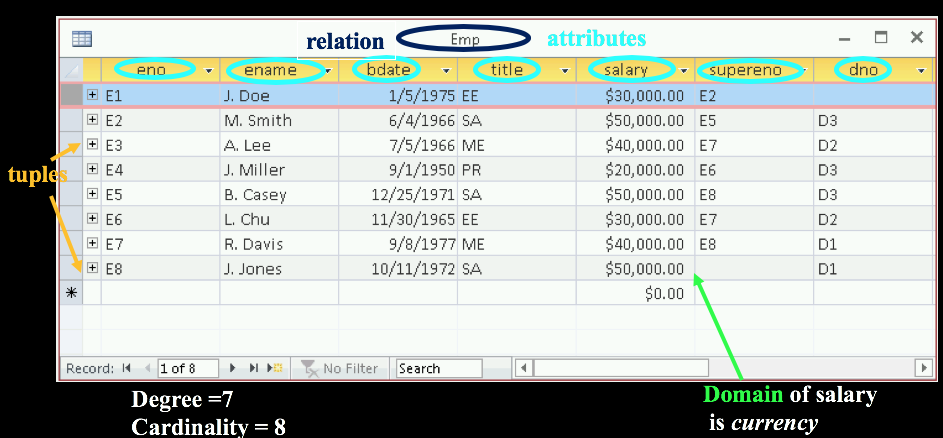
\includegraphics[width=1.\textwidth]{img/databases.png}

{\bf Side note:} 
Sometimes, the term \define{field} and \define{attribute} are used interchangeably, and for most purposes, they are the same thing. However, field describes a particular cell in a table found on any row, while attribute describes an entity characteristic in a design sense. \href{https://www.lifewire.com/attribute-definition-1019244}{[Source]}.  Eg.  {\tt A. Lee} is a \textit{field} while {\tt ename} is the  \textit{attribute}.

\end{frame}


\begin{frame}{Relation Practice Example}
$$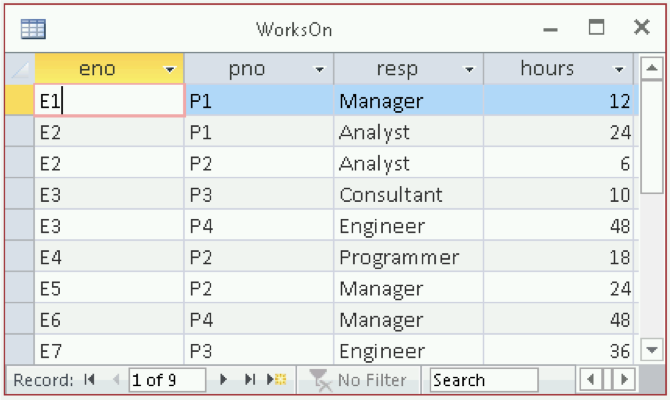
\includegraphics[width=0.5\textwidth]{img/dbq}$$
\begin{example}
\begin{enumerate}
\item What is the name of the relation?
\item What is the cardinality of the relation?
\item  What is the degree of the relation?
\item  What is the domain of resp? What is the domain of hours?
\end{enumerate}
\end{example}
\end{frame}


\begin{frame}<handout:0>{Relation Practice Example}
$$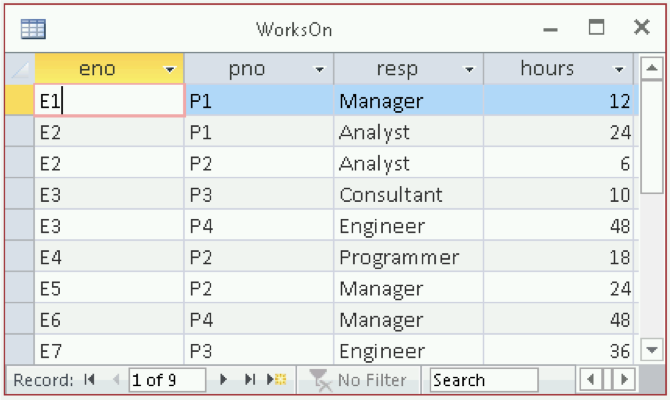
\includegraphics[width=0.5\textwidth]{img/dbq}$$
%\begin{block}
\vspace{-0.5em}
\begin{block}{Answer}
\begin{enumerate}
\item What is the name of the relation? \uncover<1->{\textit{WorksOn}}
\item What is the cardinality of the relation?  \uncover<2->{\textit{9}}
\item What is the degree of the relation? \uncover<3->{\textit{4}}
\item  What is the domain of {\tt resp}? \uncover<4->{\textit{string}}
\item  What is the domain of hours? \uncover<5->{\textit{integer}}
\end{enumerate}
\end{block}
\end{frame}

\begin{frame}{Database Definition Question}
\begin{exampleblock}
{Question:}
 How many of the following statements are TRUE?
\begin{enumerate}
\item A database  refers to the stored data.
\item  A database system refers to the software.
\item  A database system will lose the data stored when the power is turned off. 
\end{enumerate}
\begin{multicols}{4}
\begin{enumerate}[A)]
\item 0 
\item 1
\item 2
\item 3
\end{enumerate}
\end{multicols}
\end{exampleblock}
\end{frame}

\begin{frame}<handout:0>{Database Definition Question}
\begin{block}
{Answer:}
 How many of the following statements are TRUE?
\begin{enumerate}
\item {\color<1->{ForestGreen}{A database refers to the stored data.}}
\item {\color<2->{ForestGreen}{ A database system refers to the software.}}
\item {\color<3->{red}{ A database system will lose the data stored when the power is turned off. }}
\end{enumerate}
\begin{multicols}{4}
\begin{enumerate}[A)]
\item 0 
\item 1
\item \textbf<3>{\textit<3>{{\color<3>{iyellow}{2}}}}
\item 3
\end{enumerate}
\end{multicols}
\end{block}
\end{frame}


\begin{frame}{Database Definition Question}
\begin{exampleblock}
{Question:}
 How many of the following statements are TRUE?
\begin{enumerate}
\item  Usually, more than one user can use a database system at a time.
\item  The cardinality is the number of rows in a relation.
\item  A relation's cardinality is always bigger than its degree.
\end{enumerate}
\begin{multicols}{4}
\begin{enumerate}[A)]
\item 0 
\item 1
\item 2
\item 3
\end{enumerate}
\end{multicols}
\end{exampleblock}
\end{frame}


\begin{frame}<handout:0>{Database Definition Question}
\begin{block}
{Answer:}
 How many of the following statements are TRUE?
\begin{enumerate}
\item  {\color<1->{ForestGreen}{Usually, more than one user can use a database system at a time.}}
\item  {\color<2->{ForestGreen}{The cardinality is the number of rows in a relation.}}
\item {\color<3->{red}{ A relation's cardinality is always bigger than its degree.}}
\end{enumerate}
\begin{multicols}{4}
\begin{enumerate}[A)]
\item 0 
\item 1
\item \textbf<3>{\textit<3>{{\color<3>{iyellow}{2}}}}
\item 3
\end{enumerate}
\end{multicols}
\end{block}
\end{frame}




\begin{frame}{Database Definition Matching Question}
\begin{exampleblock}{Question: }
Given the three definitions, select the ordering that contains their related definitions to the following three terms: relation, tuple, attribute
\begin{enumerate}[A)]
\item  column, row, table
\item  row, column, table
\item  table, row, column
\item table, column, row
\end{enumerate}
\end{exampleblock}
\end{frame}

\begin{frame}<handout:0>{Database Definition Matching Question}
\begin{block}{Answer: }
Given the three definitions, 
Select the ordering that contains their related definitions to the following three terms: relation, tuple, attribute
\begin{enumerate}[A)]
\item  column, row, table
\item  row, column, table
\item  \answer{table, row, column}
\item table, column, row
\end{enumerate}
\end{block}
\end{frame}



\begin{frame}{Cardinality and Degree Question}
\begin{exampleblock}
{Question: }A database table has 5 rows and 10 columns.  Select one true statement.
\begin{enumerate}[A)]
\item The table's degree is 50.
\item  The table's cardinality is 5.
\item  The table's degree is 5.
\item  The table's cardinality is 10.
\end{enumerate}
\end{exampleblock}
\end{frame}



\begin{frame}<handout:0>{Cardinality and Degree Question}
\begin{block}
{Question: }A database table has 5 rows and 10 columns.  Select one true statement.
\begin{enumerate}[A)]
\item The table's degree is 50.
\item  \answer{The table's cardinality is 5.}
\item  The table's degree is 5.
\item  The table's cardinality is 10.
\end{enumerate}
\end{block}
\end{frame}



\begin{frame}{Creating and Using Databases}
Typically, a data analyst will use an existing database.  The database will already be created on a database system and contain data that was inserted and updated previously.\nl

To use an existing database, the data analyst must be able to use the tools and languages to query the database.  The standard is SQL.\nl

Creating a large database is outside of the scope of this class, but we will learn how to create individual tables and load data into them which is a common data analysis task.

\end{frame}


\begin{frame}{A Simple Query Language: Keyword Seaching}
%\emph{Keyword} (or English-language) \emph{search} 
A query on Google, for example, 
allows a user to type keywords or phrases and returns a best answer estimate.
\begin{figure}[htbp]
\begin{center}
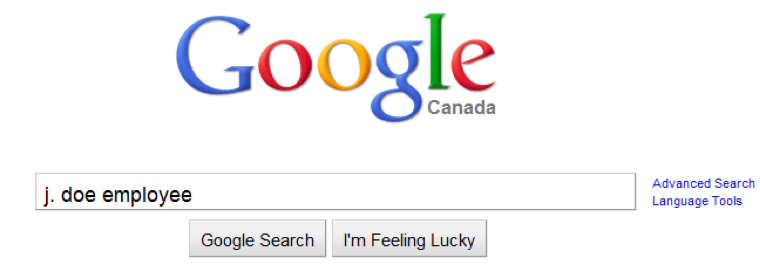
\includegraphics[width=0.6\textwidth]{img/google}
\end{center}
\end{figure}



This works fairly well for web searches, although we lack precision.  Precision is required for many applications.\\
\begin{itemize}
\item Example: How would you return all employees with salary greater than 30,000 using keyword search?
\end{itemize}
\end{frame}

\section{SQL}
\begin{frame}{SQL Overview}
\define Structured \define Query \define  Language or \define{SQL} is the standard database query language to retrieve \emph{exact answers}.\medskip
\begin{itemize}
\item Using simple, declarative \emph{statements} (i.e. a valid command recognized by the database), SQL queries specifies \textit{what to} retrieve %but not \textit{how} to retrieve it.
while preserving the accuracy, security and integrity of the database.\medskip
%\item   % This keeps data accurate and secure, and helps maintain the integrity of databases, regardless of size.
\item SQL is used by Microsoft Access, LibreOffice Base, and almost all other database systems.\medskip
\item A knowledge of SQL commands will give you the power to access and explore data stored or relational databases.
\end{itemize}
\end{frame}

\begin{frame}{SQL Overview}

%Some basic rules for SQL statements:\medskip
\begin{itemize}
\item There is a set of \emph{reserved/key words} that cannot be used as names for database fields and tables. e.g. \command{SELECT, FROM, WHERE}, etc.\medskip

\item SQL is generally \emph{case-insensitive}.
\begin{itemize}
\item  \command{SELECT} will be treated the same as \command{Select} and \command{select}\footnote{standard convention usually will capitalize keywords}
\item Some setups are case-sensitive for table and column, for example, %https://stackoverflow.com/questions/153944/is-sql-syntax-case-sensitive
%\item  Only exception is string constants, 
 {\tt `ENAME'} not the same as {\tt `ename'}.
\item Linux MySQL:  usually defaults to case-sensitive for table and column names 
\item Windows: usually defaults to case-insensitive for table and column names 
\item  Note that  LibreOffice Base converts unquoted fields and table names to upper case; more on this \href{https://eeperry.wordpress.com/2013/11/15/libreoffice-base-sql-creating-tables/}{here}.
\end{itemize}
\medskip
\item SQL is \emph{free-format} and white-space is ignored.\medskip
\item Statements always end in a semicolon {\tt ;}
\end{itemize}
\end{frame}


%\begin{frame}
%SQL is a {\bf declarative language} (non-procedural). \nl
%
%SQL first became an official standard in 1986 as defined by the American National Standards Institute (ANSI).\nl
%All major database vendors conform to the SQL standard with minor variations in syntax (different dialects).
%SQL consists of both a Data Definition Language (DDL) and a Data Manipulation Language (DML).
%
%An SQL identifier (name) must follow these rules:
%only contain upper or lower case characters, digits, and underscore ("_") character
%be no longer than 128 characters. DB vendors may impose stricter limits than this.
%must start with a letter (or underscore)
%cannot contain spaces
%Note: Quoted or delimited identifiers enclosed in double quotes allow support for spaces and other characters.  E.g. "select"
%
%\end{frame}





\begin{frame}{SQL Create Table}\label{createtab}
The \command{CREATE TABLE} \define{command/clause}  is used to create a table in the database. \begin{itemize}
\item A \textit{\bf clause/command} performs a  specific tasks in SQL. While clause will work with lowercase letters, the convention is to write command in capital letters. 
\end{itemize}
 A table consists of a table name (eg. {\tt emp}) and a set of fields/attributes with their names and data types (i.e. domain).
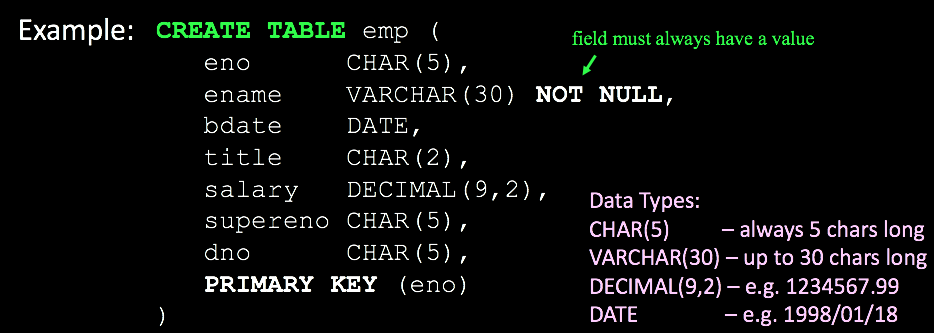
\includegraphics[width=1.\textwidth]{img/createTab.png}
\end{frame}



\begin{frame}{SQL Create Table - Constraints}
\begin{itemize}
\item The {\tt NOT NULL}  is a \emph{constraint} which indicates that we can not enter a tuple into this relation without the field {\tt ename}
\medskip
\item To put another way, all employees in the employee table must be entered with an employee name (makes sense!)
\medskip
\item Other constraints include:
\begin{description}
\item[{\tt UNIQUE}]  forces all rows to have a different value.
\item[{\tt DEFAULT}] sets the field to a certain value if it is not specified, 
\begin{itemize}
\item[eg.] {\tt DEFAULT 0} or {\tt DEFAULT 'unknown'} 
\end{itemize}

\end{description}

\end{itemize}
\end{frame}


\begin{frame}{What is a key?}
A \define{key} is a set of attributes that \emph{uniquely} identifies a tuple in a relation. Read more about this constrain \href{https://www.w3schools.com/sql/sql_primarykey.asp}{here}
\begin{itemize}
\item A \emph{primary key} uniquely identifies a record in the table. 
\item A table can have only \alert{one} primary key; however it can consist of single or multiple columns (fields).
\item A \emph{foreign key} is a field in a table that is primary key in another table. 
\end{itemize}


Although keys are not required, they can help to identify a particular row (data item) and find it faster.\nl

In the {\tt emp} table, the key was {\tt eno}.  It was called the {\tt primary key} because it was the main key used to find an employee in the table.\nl

%Although primary keys are required in LibreOffice base GUI, they are not required in general.\nl
\begin{exampleblock}
{Question:}
What is a key to identify a student in this class?
\end{exampleblock}


\end{frame}
%Use example with trying to find person in class. If give system a first name, do you always get one person back?
%
%Possible verbal example: Person(SSN,Name,Age)
%Introduce StudentId as a candidate key for a university person database. Candidate keys at UBC: SIN, StudentId, 
%Not keys: lastname, lastname/firstname (maybe)
%
%Useful to emphasize the difference between minimal - cannot remove any attribute and still be a superkey and minimum which is the minimum # of attributes in a key.  There can be two keys: one with one attribute and another with two attributes.  They are both minimal in the sense that you cannot remove any attribute and still be a key.
%
%Can also use example of a course key: department number, course number, section number




\begin{frame}[fragile]{{\tt CREATE TABLE} Syntax}
The general syntax to create a new table in a database:
\begin{Verbatim}[frame=single, xleftmargin=2cm, xrightmargin=2cm, commandchars=\\\{\}]
\purple{CREATE TABLE} table_name (
    attribute1 datatype,
    attribute2 datatype,
    ...
);
\end{Verbatim}
We specify the names of the columns of our table within the parenthesis
\begin{itemize}
\item notice that they are separated by commas 
\item end of lines have a semicolons 
\item We can choose from a number of \href{https://www.w3schools.com/sql/sql_datatypes.asp}{data types} (e.g. varchar, integer, date, etc.).\nl
\end{itemize}
\end{frame}

\begin{frame}[fragile]{{\tt CREATE TABLE} Syntax in LibreOffice Base}
In LibreOffice Base, unquoted fields and table names are converted to upper case. \href{https://eeperry.wordpress.com/2013/11/15/libreoffice-base-sql-creating-tables/}{read more here}.\\
\medskip
To prevent this, you can use quoted attribute and tables names, eg.
\begin{Verbatim}[frame=single, xleftmargin=2cm, xrightmargin=2cm, commandchars=\\\{\}]
\purple{CREATE TABLE} "table_name" (
    "attribute1" datatype,
    "attribute2" datatype,
   ....
);
\end{Verbatim}


\end{frame}


% https://www.codecademy.com/courses/learn-sql/lessons/manipulation/exercises/statements?action=resume_content_item
%(column_1 data_type, column_2 data_type, column_3 data_type) is a parameter. A parameter is a list of columns, data types, or values that are passed to a clause as an argument. Here, the parameter is a list of column names and the associated data type.
%CREATE TABLE celebs (
%   id INTEGER, 
%   name TEXT, 
%   age INTEGER
%);
% (id INTEGER, name TEXT, age INTEGER) is a list of parameters defining each column, or attribute in the table and its data type:
%
%id is the first column in the table. It stores values of data type INTEGER
%name is the second column in the table. It stores values of data type TEXT
%age is the third column in the table. It stores values of data type INTEGER









\begin{frame}{Try It: {\tt CREATE TABLE}}
\begin{exampleblock}{Question:} Create a table called {\tt mydata} that has three fields:
\begin{itemize}
\item {\tt num} -- that will store a number (use {\tt int} as data type)
\item {\tt message} -- that will store a string up to 50 characters ({\tt varchar} data type)
\item {\tt amount} -- that stores a decimal number with 8 total digits and 2 decimal digits (decimal data type)
\end{itemize}
Use the web site \yellow{\bf sqlfiddle.com} or \href{https://www.db-fiddle.com/}{DB-fiddle} to try your table creation.
\end{exampleblock}
SQL fiddle is an online SQL database (no need to download anything) where we can test, debug and share SQL snippets.
Sharing is as easy as pasting the url.
\href{http://sqlfiddle.com/\#!9/d8ad4/3}{click me!}
 %\verb|http://sqlfiddle.com/#!9/b9363|
%Sharing is as easy as this pasting the url: \href{http://sqlfiddle.com/#!9/5a251b}{click me}
\end{frame}
% The empty "Persons" table can now be filled with data with the SQL INSERT INTO statement.



\begin{frame}\ft{Relational Database Management Systems}
In this lecture we will be introducing a couple relational database management systems. 
\begin{itemize}
\item UBC qualify for a free \href{https://it.ubc.ca/services/desktop-print-services/software-licensing/office-365-students}{Office 365} subscription, which includes free downloads of: Word, Excel, PowerPoint, and more. 
\item Students running Windows can also install \define{Microsoft Access}.
\item Microsoft Access is a Database Management System (DBMS).
\item Access can work directly with data from %other sources, including many popular PC database programs, with 
many SQL databases on the desktop, on servers, on minicomputers, or on mainframes, and with data stored on web servers.
\end{itemize}
\href{https://www.tutorialspoint.com/ms_access/ms_access_overview.htm}{TutorialsPoint} is a great resource for help on MS Access.
\end{frame}



\begin{frame}\ft{Relational Database Management Systems}
For students \textit{not} running Windows, a nice alternative is \emph{LibreOffice}
\begin{itemize}
\item  \emph{LibreOffice} is a free and open-source office suite, a project of The Document Foundation. 
\item \define{LibreOffice Base} is a free and open-source relational database management system that is part of the LibreOffice office suite; download \href{https://www.libreoffice.org/download/download/}{here}
\item Like Access, it can be used to create and manage databases either locally or on servers eg. {\bf mysql,} an {\bf access database}.
\end{itemize}
\medskip
As I am using a Mac, I will be conducting demonstrations in LibreOffice Base.  The details for Microsoft Access are provided as snap shots throughout and will be very similar to LibreOffice Base.
\begin{itemize}
\item \href{https://thefrugalcomputerguy.com/seriespg.php?ser=15/}{Here} is a useful webpage for help on LibreOffice Base along with the \href{https://wiki.documentfoundation.org/images/e/e8/BH40-BaseHandbook.pdf}{handbook}.
\end{itemize}

\end{frame}



\begin{frame}\ft{Relational Database Management Systems}
\begin{itemize}
\item We will learn how to code SQL queries.
\item Queries offer the ability to retrieve and filter data, calculate summaries (totals), and update/move/delete records in bulk.
\item We also may want to take advantage of the graphical user interface (GUI)  frontend for data manipulation and queries.
\item These visual representations % of tables and the graphical links between them makes Microsoft Access queries extremely
are easy to use and hides the complexity of writing SQL commands while still providing access to  powerful and advanced analysis
\item   We'll see how we can easy switch between the graphical query design and SQL syntax. 
\item Bonus: this easy back and forth may be useful as you are trying to learn SQL.
\end{itemize}
\end{frame}



\begin{frame}{CREATE TABLE in Microsoft Access}
In Microsoft Access, start by  creating a ``Blank desktop database" (give it whatever name you want).\\
\begin{center}
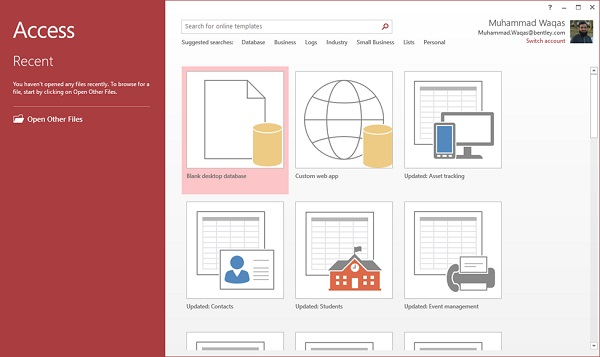
\includegraphics[width=0.9\textwidth]{img/blankDatabase.jpg}
\end{center}
\href{https://www.tutorialspoint.com/ms_access/ms_access_create_database.htm}{Image source}
\end{frame}


\begin{frame}{CREATE TABLE in Microsoft Access}
Next,  navigate to the {\bf Create} tab in the Ribbon and select the {\bf Table} button \ 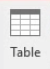
\includegraphics[width=2em]{img/create_tab.png}\  to build a table.  To get to the ``Design View" as seen on the next page, go to {\bf View} $>$ {\bf Design View} in the {\bf Fields} tab:
\\
\begin{center}
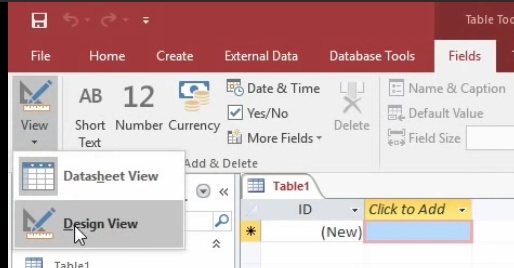
\includegraphics[width=0.5\textwidth]{img/designView}
\end{center}
For a walk through of this, see \href{https://www.youtube.com/watch?v=PBhftKTmdHI}{this} demo on YouTube.
\end{frame}



\begin{frame}{CREATE TABLE in Microsoft Access}
\begin{center}
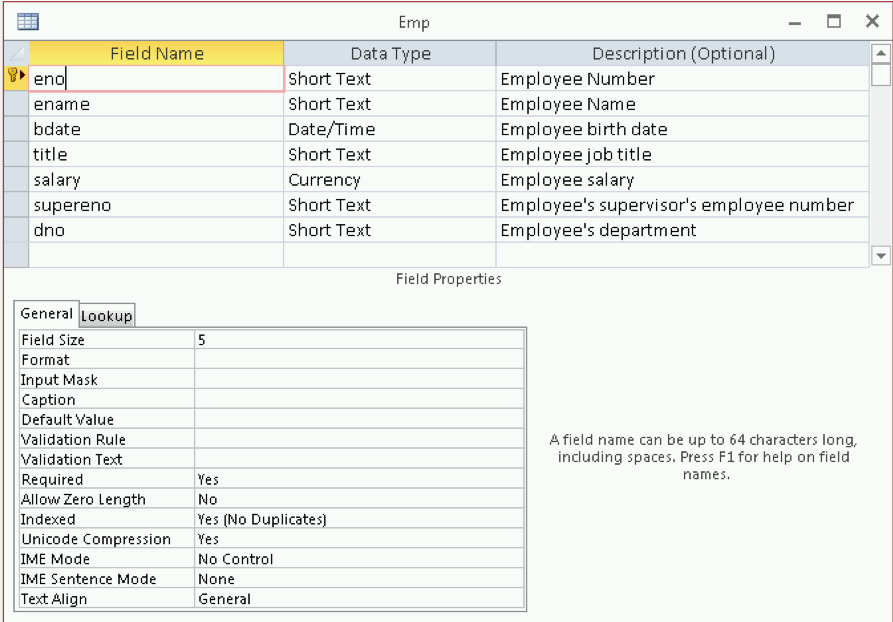
\includegraphics[width=0.9\textwidth]{img/createTable}
\end{center}
\end{frame}


\begin{frame}{CREATE TABLE in LibreOffice Base}
Upon opening Base, a database Wizard will pop-up.  While we could access an existing database from a server, today we will be creating a new internal database:
\begin{center}
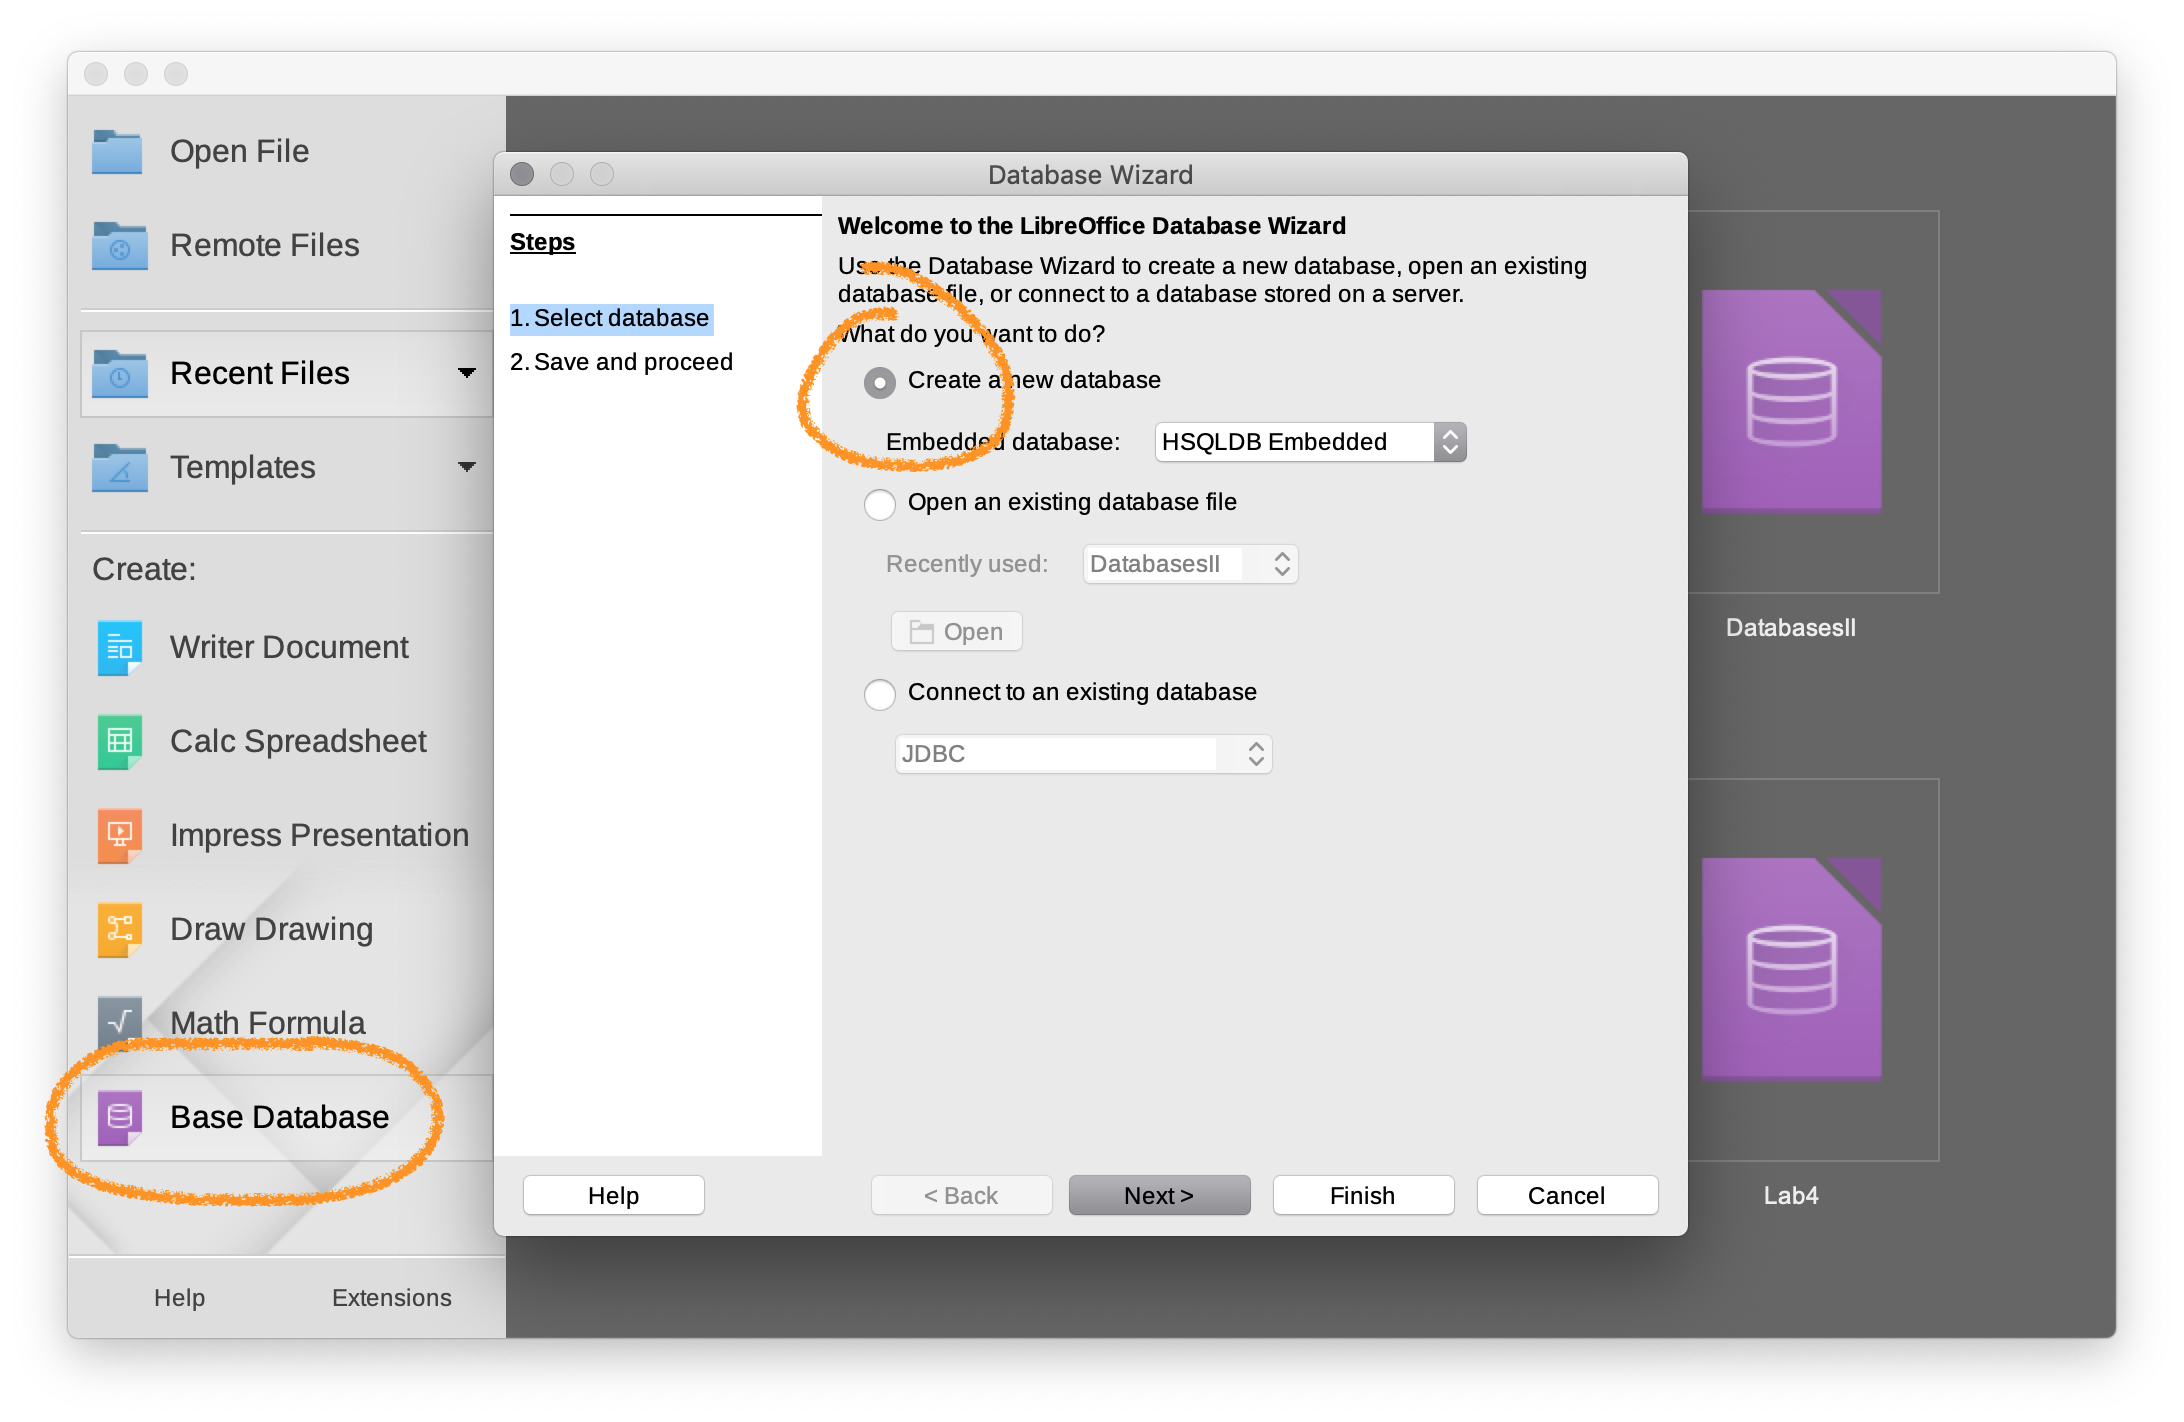
\includegraphics[width=0.9\textwidth]{img/LibreOffice1}
\end{center}
\end{frame}


\begin{frame}{CREATE TABLE in LibreOffice Base}
\begin{itemize}
\item If you don't see the Database Wizard, choose {\bf File}  $>$  {\bf New} $>$ {\bf Database}. (Shortcut \keystroke{Cmnd} + \keystroke{N}).
\medskip
\item To create a new database file.
\begin{enumerate}
\item select the type of database (leave the HSQLDB environment default), 
\item you may or may not choose to register you database\footnote{registered databases be accessed by other program components as a data source (e.g. \href{https://thefrugalcomputerguy.com/grouppg.php?ser=15&grp=26\#}{mail merge}}.  For now choose no (we can always register it later).
\item click the %option to open the Table Wizard as the next wizard.
{\bf Finish} button.
\end{enumerate}
\bigskip
N.B. The Table Wizard helps you to add a sample tables  to the new database file upon which we can build; see \href{https://documentation.libreoffice.org/assets/Uploads/Documentation/en/GS5.2/HTML/GS5208-GettingStartedWithBase.html}{ \textit{Using the Wizard to create a table}}.
\end{itemize}
\end{frame}


\begin{frame}{CREATE TABLE in LibreOffice Base}
It doesn't make any functional difference to us if we register the database for what we will be doing.  Either leave it at the default or change it to ``No, do not register the database".
\begin{center}
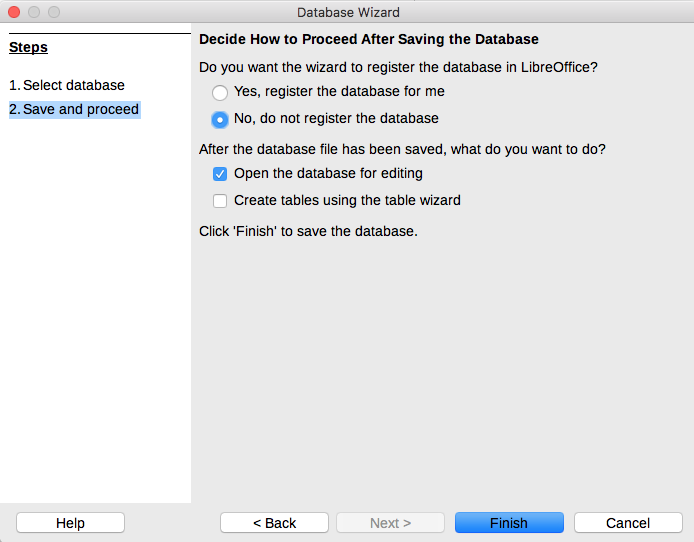
\includegraphics[width=0.9\textwidth]{img/lob}
\end{center}
\end{frame}


\begin{frame}{CREATE TABLE in LibreOffice Base}
Right now we have an empty database. In LibreOffice Base use "Create a Table in Design View" to add a table.
\begin{center}
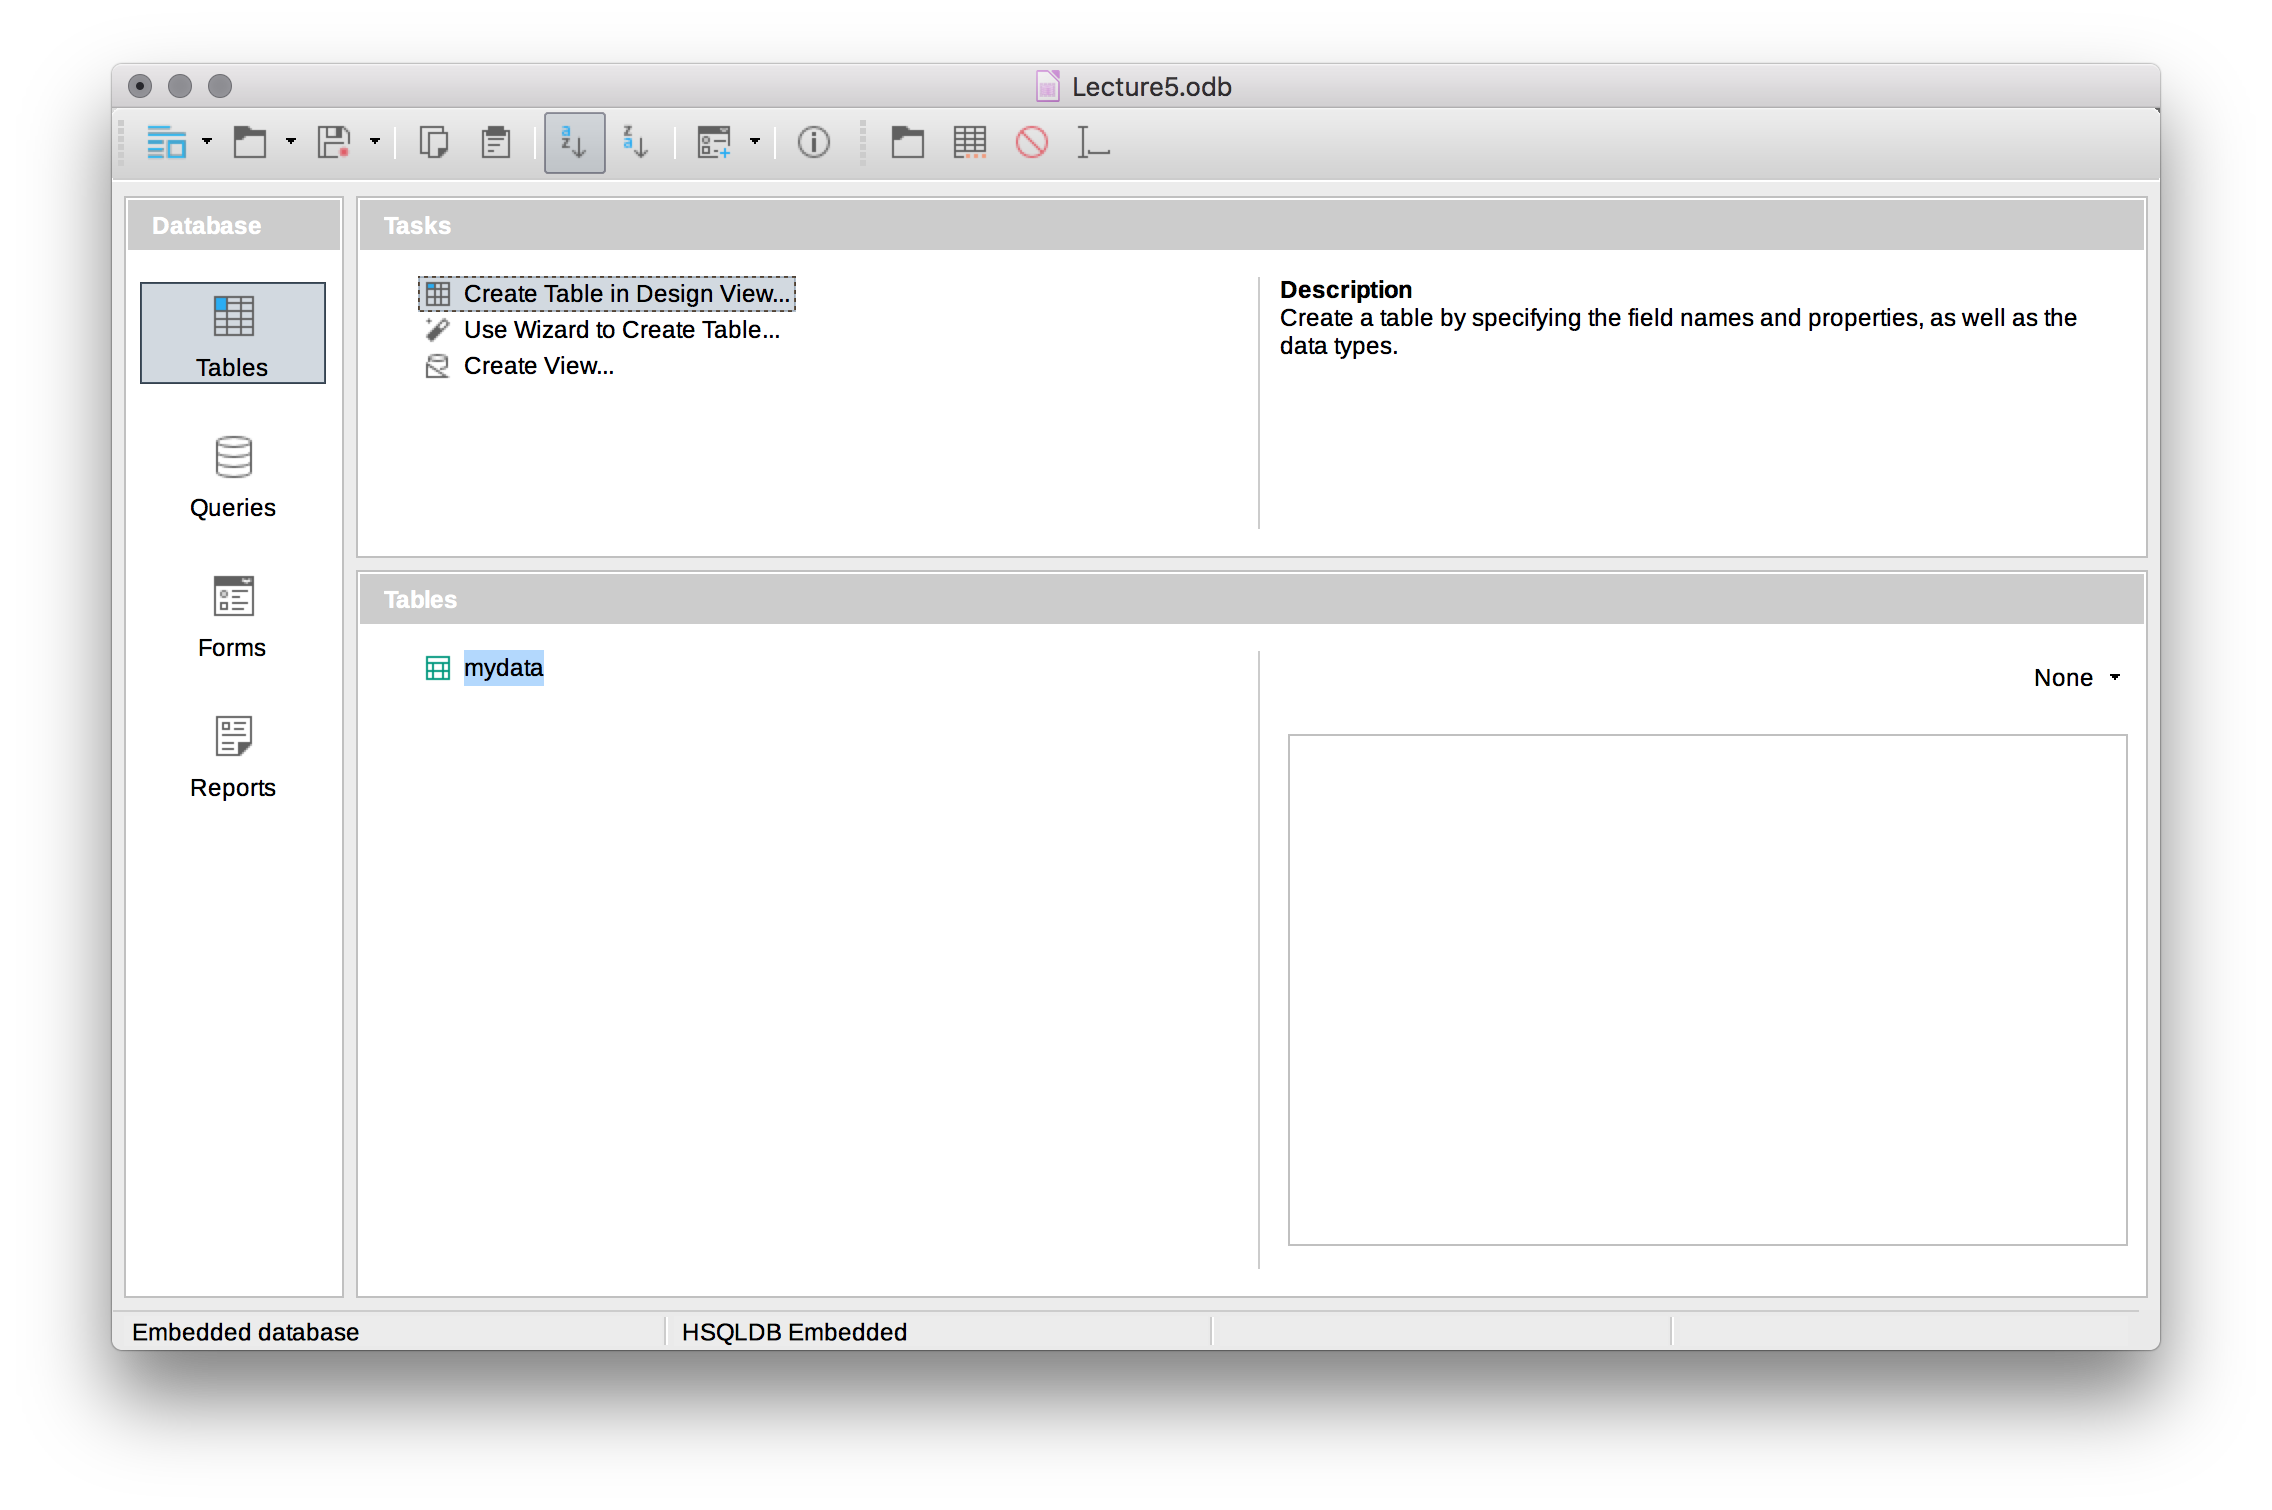
\includegraphics[width=0.9\textwidth]{img/LibreOffice}
\end{center}
\end{frame}


 \begin{frame}{CREATE TABLE in LibreOffice Base}
We can enter our fields and specify the data types from the drop down menu.  Any extra parameters can be entered in the boxes provided below. 
\begin{center}
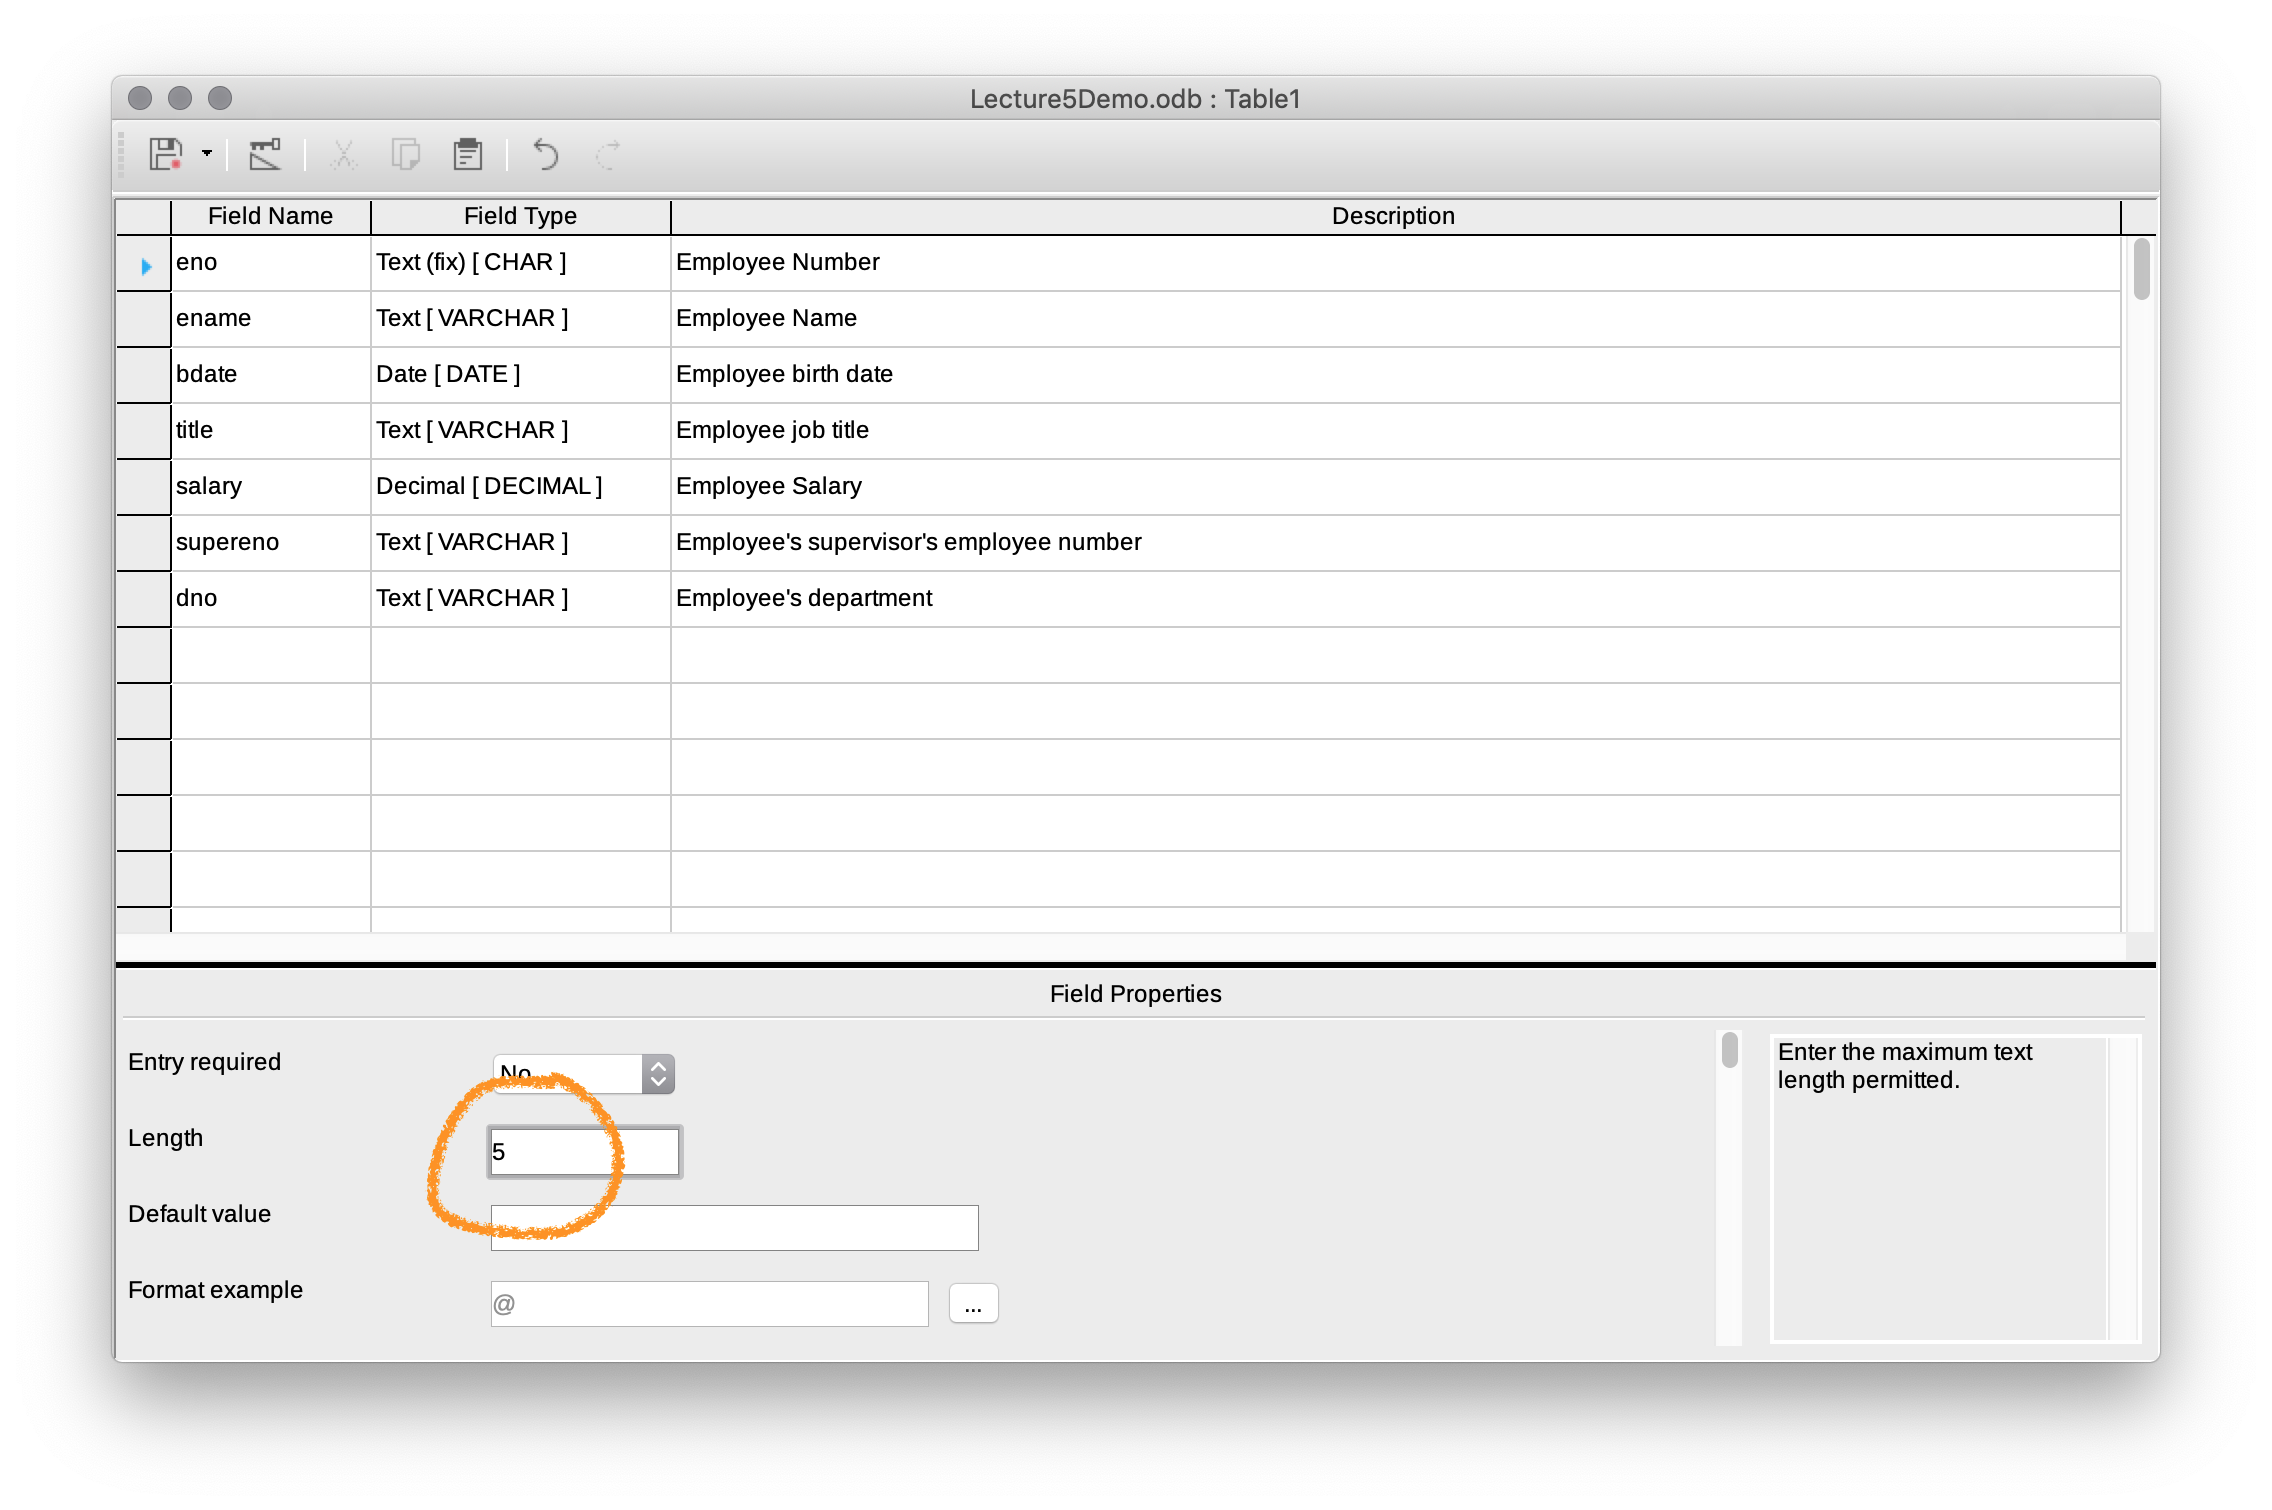
\includegraphics[width=0.9\textwidth]{img/LibreOffice3}
\end{center}
% 
\end{frame}

\begin{frame}
\begin{itemize}
\item To make an attribute a primary key in LibreOffice Base, simply right click on the Field Name and select ``Primary Key". 
\vfill
\item In MS Access, select the field and press the  primary key button 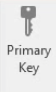
\includegraphics[width=1.5em]{img/pkey} 
\vfill
\item N.B. Data type options are named slightly different in LibreOffice Base than MS Access).
\vfill
\item For example % Compare with slide \ref{createtab}. eg, {\tt eno CHAR(5)} is specified as {\tt TEXT} with {\bf Length} 5.
``Text" vs. ``Short Text", LibreOffice base does not have a ``Currency" option.
\vfill
\item To  view the image from the previous slide, open WorksOn.odb in LibreOffice base, right click on the {\tt emp} table and press Edit
\vfill
\end{itemize}

\end{frame}



\begin{frame}{Schemas and Metadata}
%Creating tables defines the structure of the database.  \nl
%
Typically a database will be a compilation of many tables that are all connected in some way.\nl
The description of the structure of the database is called a \define{schema}. It can refer to a visual representation of a database or a set of rules that govern a database.\nl

The schema is a type of \emph{metadata}.
\begin{center}
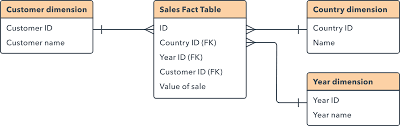
\includegraphics[width=0.9\textwidth]{img/schema}
\end{center}
\end{frame}


\begin{frame}[fragile]{Adding Data using {\tt INSERT}}
Insert a row using the \command{INSERT} command:
\begin{quote}
\begin{Verbatim}[frame=single, commandchars=\\\{\}]
\purple{INSERT INTO} emp \purple{VALUES} ('E9','S. Smith',
'1975-03-05', 'SA',60000,'E8','D1');
\end{Verbatim}
\end{quote}

Recall the fields of our table:  {\tt eno, ename, bdate, title, salary, supereno, dno}\nl

If you do not give values for all fields in the order they are in the table, you must list the fields you are providing data for:
\begin{quote}
\begin{Verbatim}[frame=single, commandchars=\\\{\}]
\purple{INSERT INTO} emp(eno, ename, salary) 
     \purple{VALUES} ('E9','S. Smith',60000);
\end{Verbatim}
\end{quote}

Note: If any columns are omitted from the list, they are set to NULL. \alert{Note that {\tt NULL} is not the same thing as an empty string} \verb!''!

\end{frame}

\begin{frame}[fragile]
\begin{exampleblock}
{Question} Using the {\tt mydata} table insert three rows: 
\begin{itemize}
\item (1, 'Hello', 99.45)
\item (2, 'Goodbye', 55.99)
\item (3, 'No Amount')
\end{itemize}

\end{exampleblock}

\begin{alertblock}{Some notes on quotes}
Notice how numbers do not need to be surrounded in quotes. While we may use single or double quotes around text, single quotes is generally preferred. 
\end{alertblock}
\begin{alertblock}{Dates}
The DATA data type appears in the format YYYY-MM-DD (in quotes) eg, \verb|bdate = '1975-01-15'|.  
\end{alertblock}
\end{frame}

\begin{frame}
Continuing from our  \href{http://sqlfiddle.com/\#!9/d8ad4/3}{sqlfiddle} example.
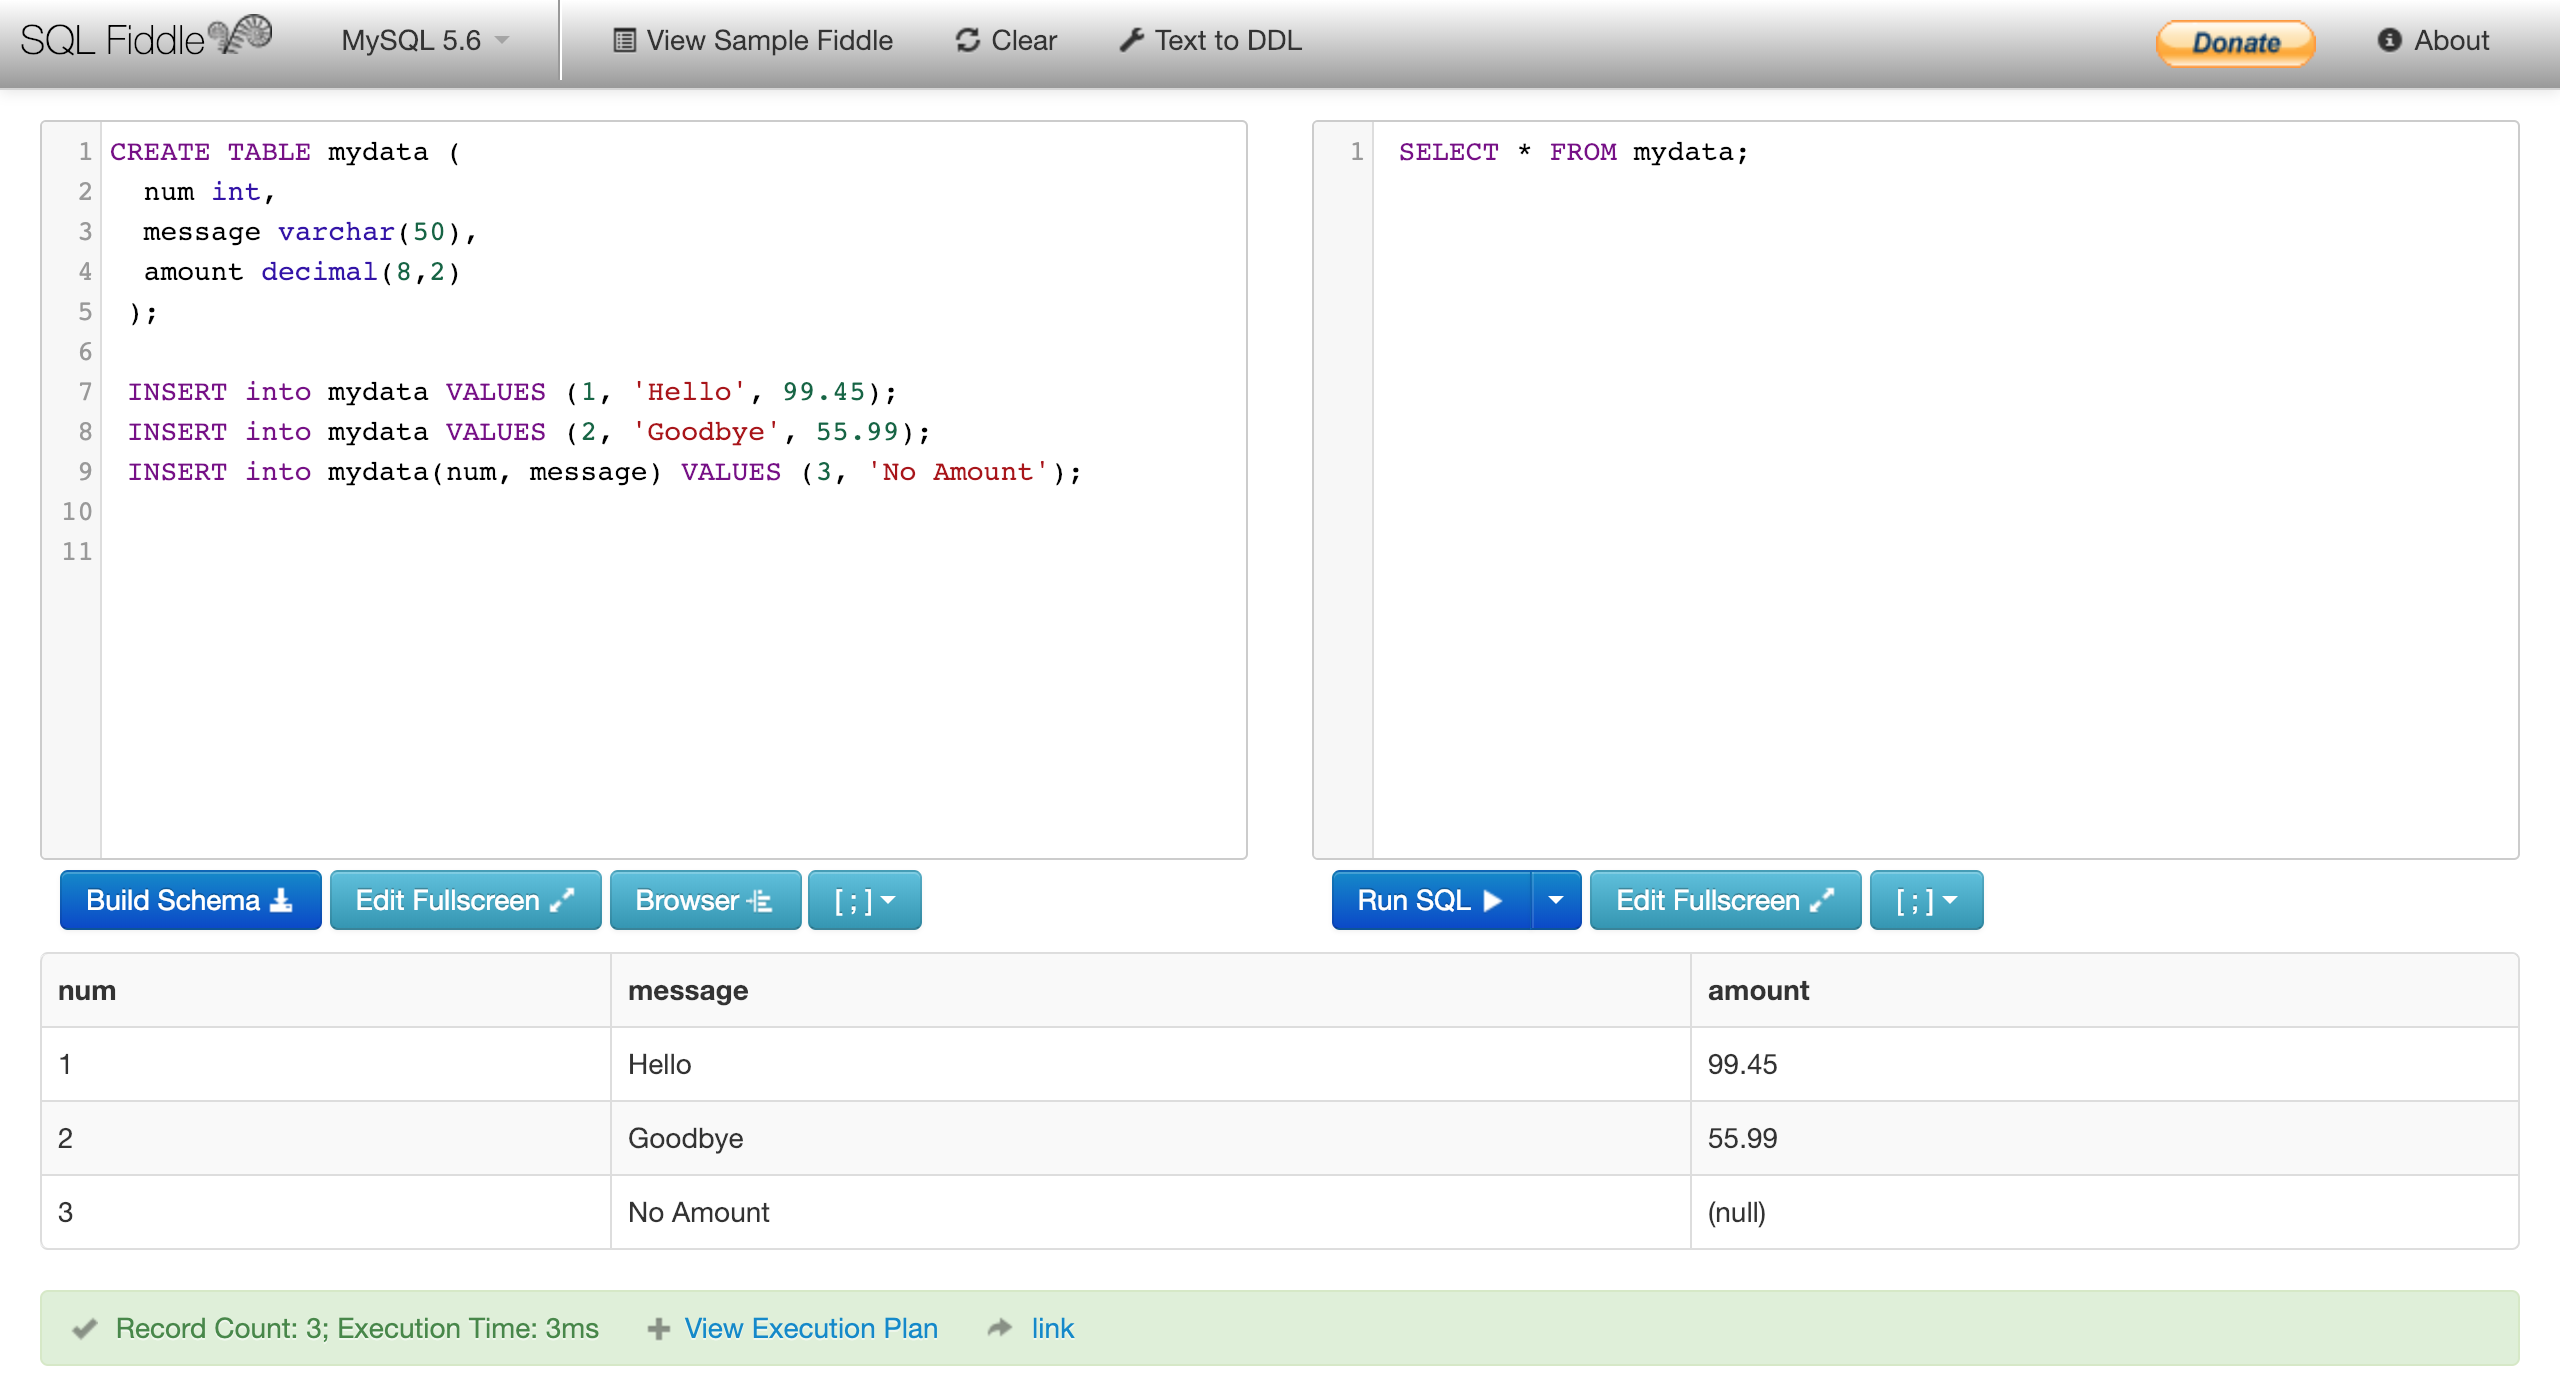
\includegraphics[width=1.01\textwidth]{img/SQLfiddle.png}\\
\begin{itemize}
\item {\tt SELECT * FROM mydata;} will return the entire {\tt mydata} table (more on this later). 
\item The {\bf Record Count} located on the green line-- this indicates the number of rows returned in our query.
\end{itemize}
\end{frame}



\begin{frame}{Adding Data in Microsoft Access }
Consider the  {\tt WorksOn.accdb}  database on Canvas. In Microsoft Access, insert a new row by entering data into the last row of the table when in data view.
\begin{center}
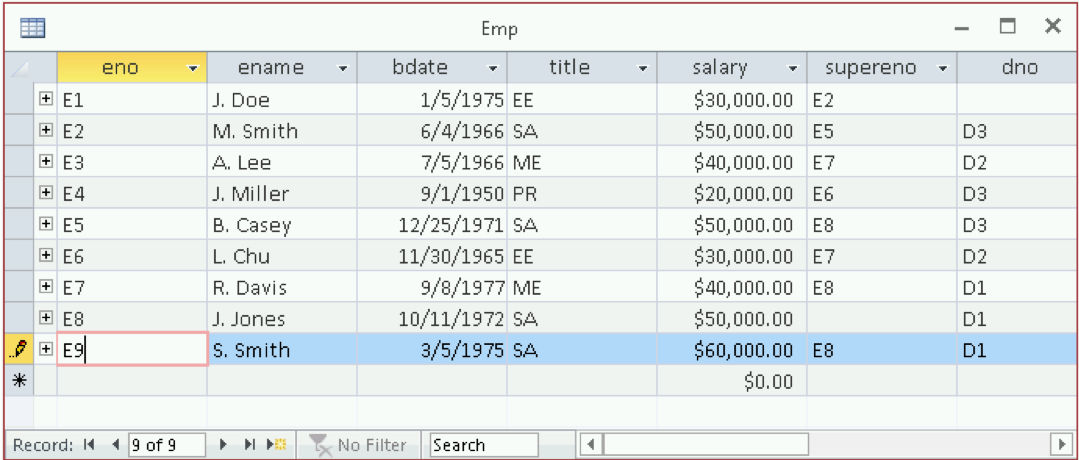
\includegraphics[width=0.9\textwidth]{img/insert}
\end{center}

\end{frame}


\begin{frame}{Adding Data in LibreOffice Base}
Consider this {\tt WorksOn.obd}, we can add a row to the {\tt emp} table by simply double clicking it in {\bf Tables} and inputting the data as we would in an Excel spreadsheet. 
\begin{center}
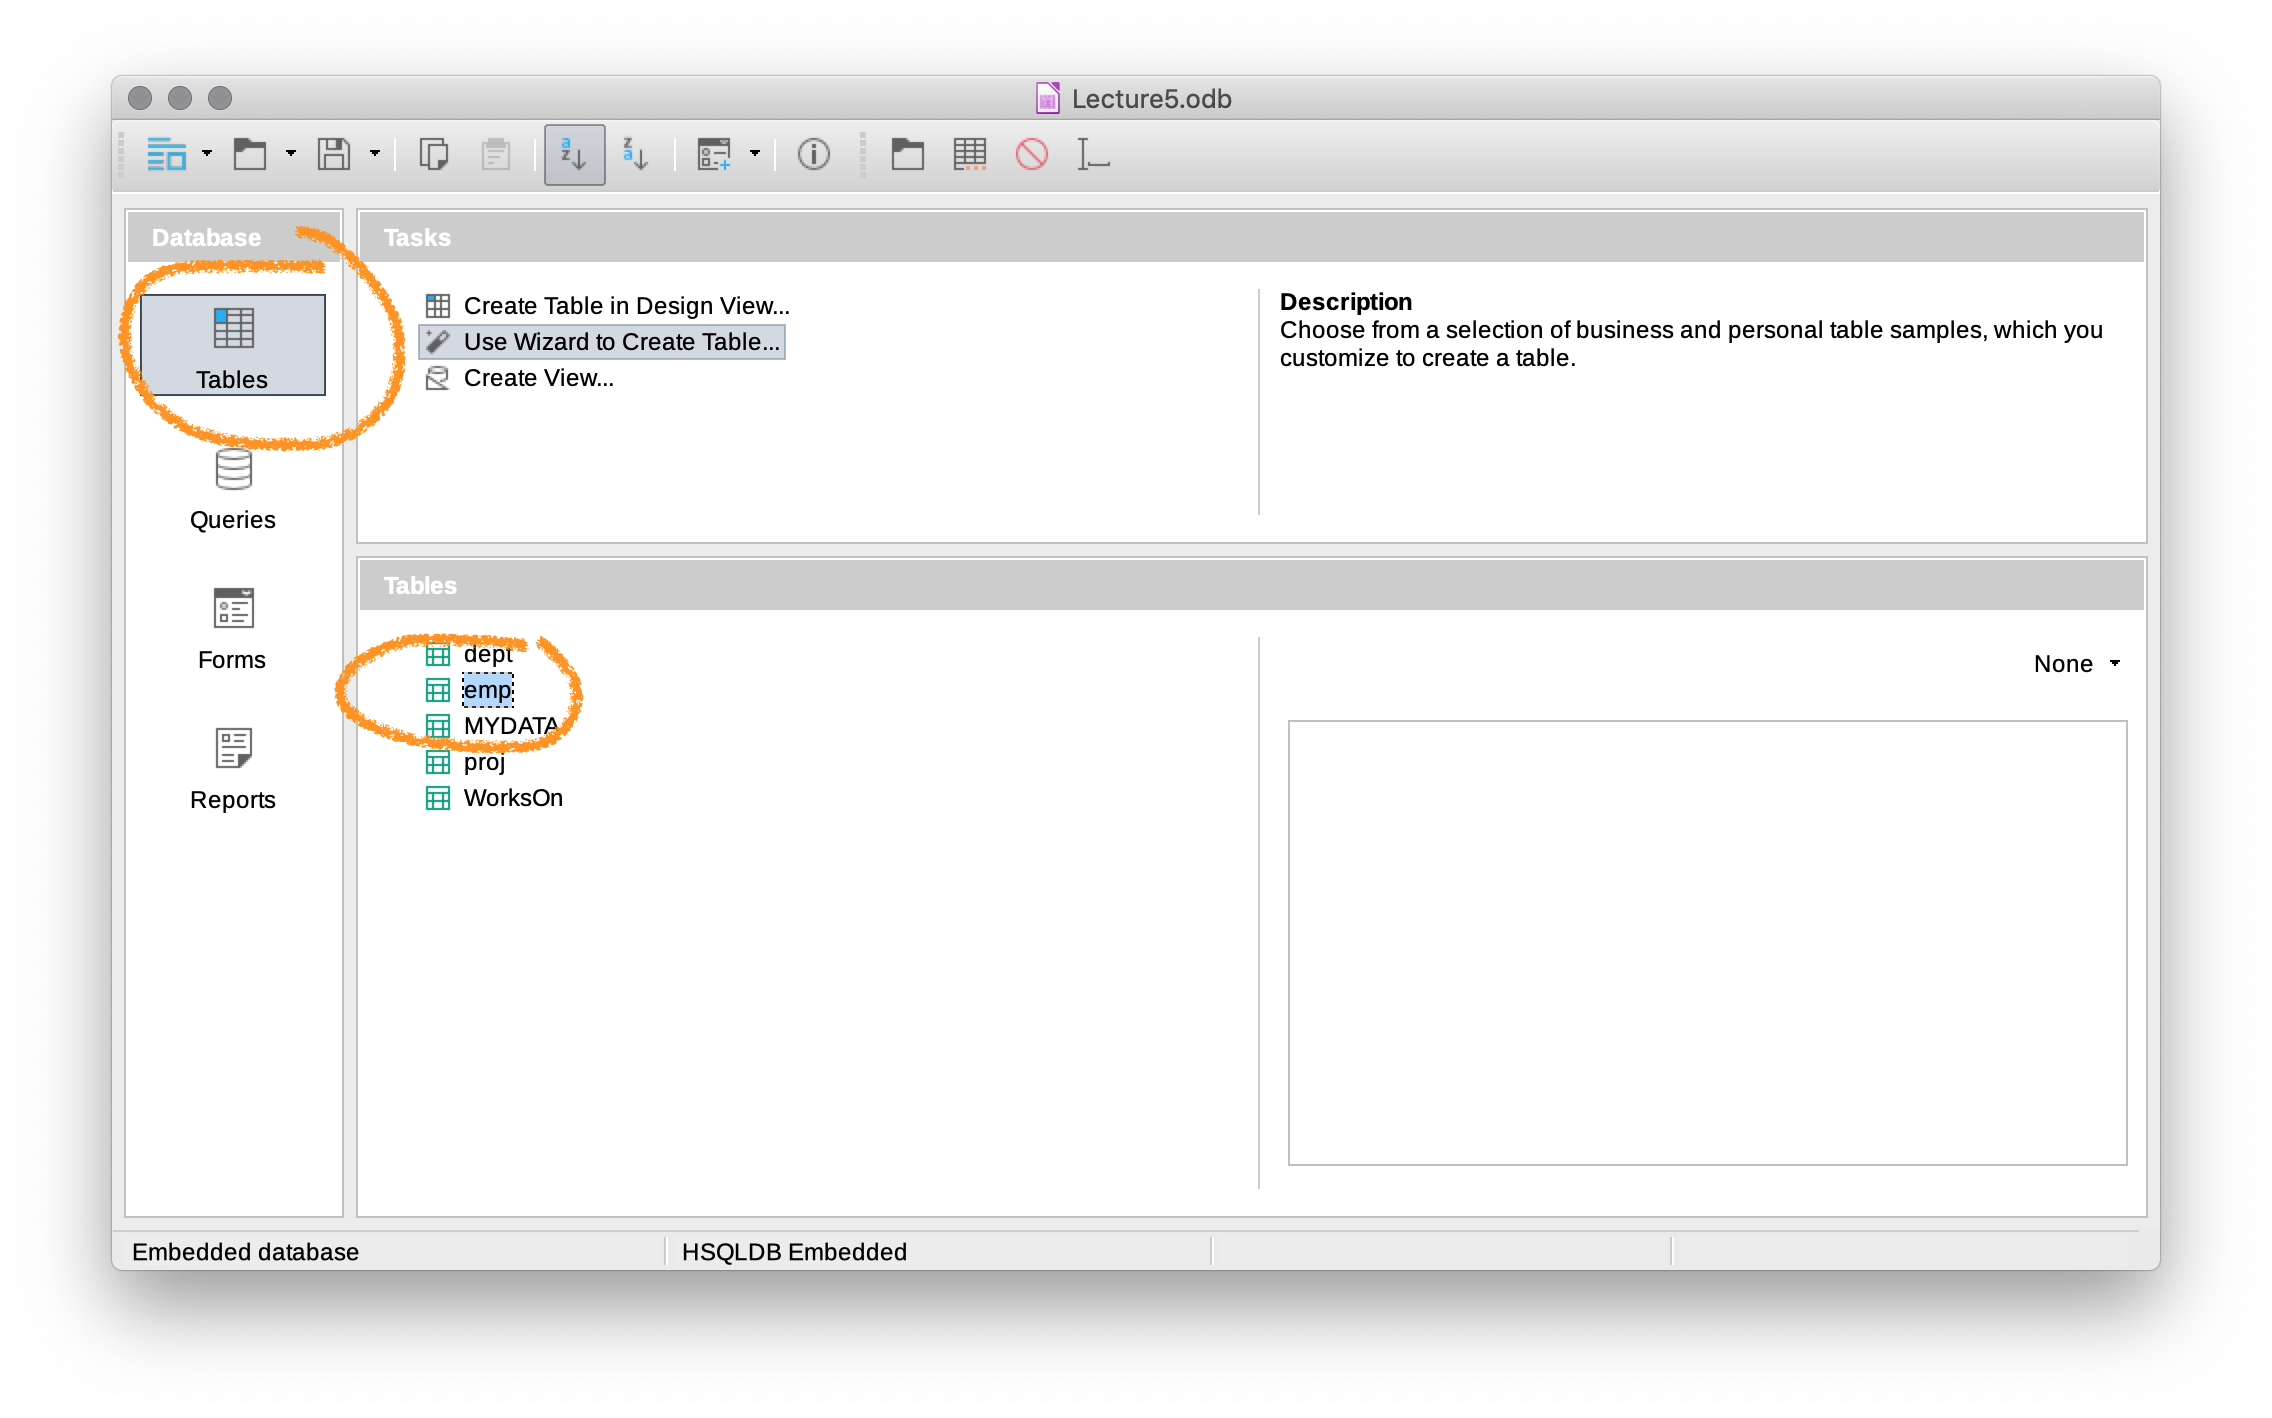
\includegraphics[width=0.9\textwidth]{img/empTables}
\end{center}
\end{frame}

\begin{frame}{Adding Data in LibreOffice Base}
Consider this {\tt WorksOn.obd}, we can add a row to the {\tt emp} table by simply double clicking it in {\bf Tables} and inputting the data as we would in an Excel spreadsheet.  N.B. You have to set a primary key before adding records to a table using this feature %https://ask.libreoffice.org/en/question/67197/how-can-i-add-a-record-to-database/
\begin{center}
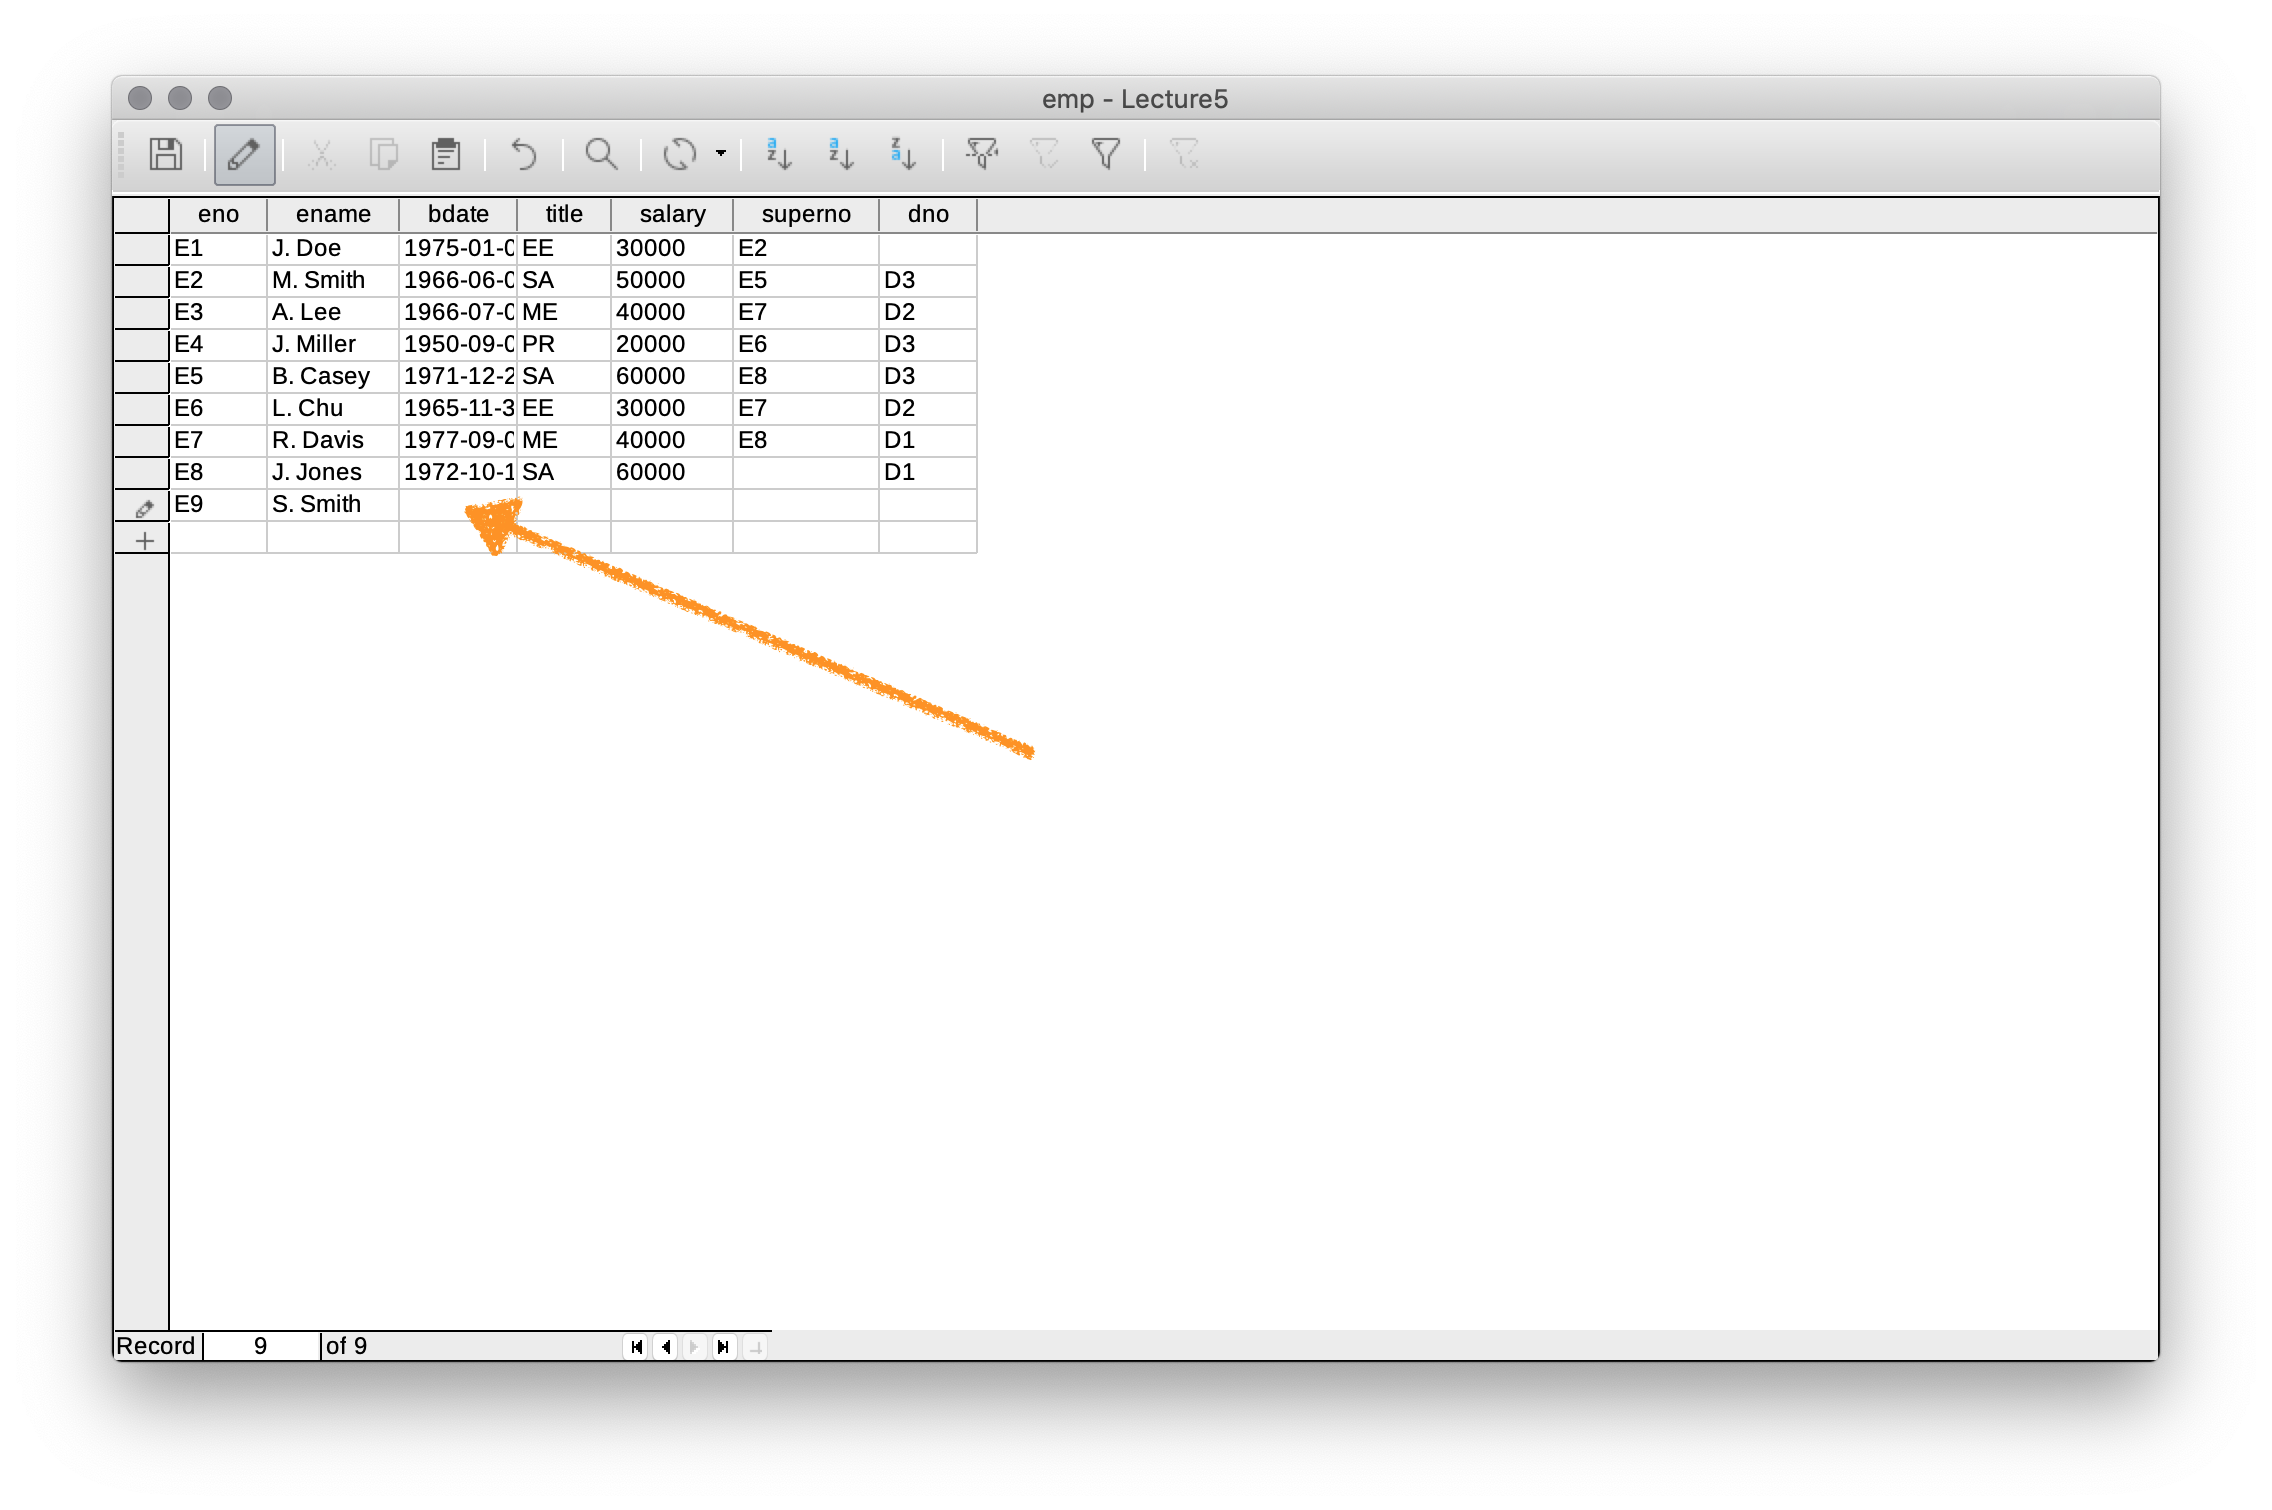
\includegraphics[width=0.9\textwidth]{img/inputEmp}
\end{center}
\end{frame}

\begin{frame}{SQL mode}
\begin{itemize}
\item Rather than using the Design View mode, we can use SQL commands by selection {\bf Tools} $>$ {\bf SQL} in LibreOffice Base.
\medskip
\item If you are using Microsoft Access, you can access SQL view by following \href{https://www.youtube.com/watch?v=IqGXE2nZZ9o}{this} demo or the instructions on \hyperlink{SQLaccess}{this} slide.
\medskip
\item  After you type in your command and press {\bf Execute}, you will get a status command to see if your command was successful or had any syntax errors:
\medskip
\item N.B. In order to see {\tt mytable} appear in the Tables panel, you may have to refresh by selection {\bf View} $>$ {\bf Refresh Tables} 
\medskip
\item \href{https://eeperry.wordpress.com/2013/11/15/libreoffice-base-sql-creating-tables/}{Recall} since I didn't put my table names and fields in quotes, they get converted to capital letters (specific to LibreOffice Base--may not be the functionality of Access).
\end{itemize}

\end{frame}

\begin{frame}{SQL mode}
\begin{center}
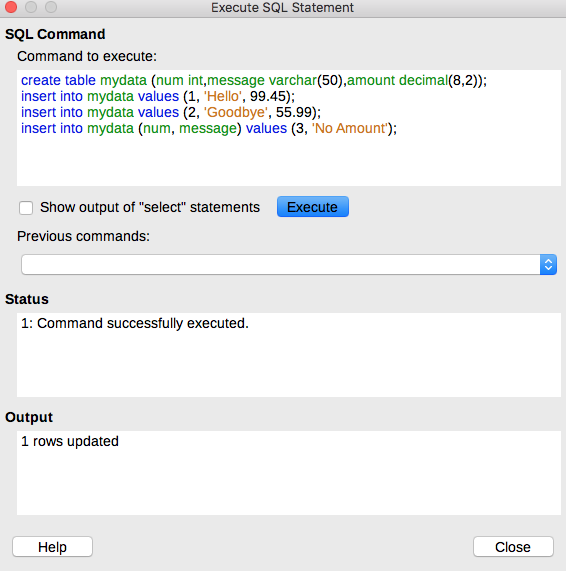
\includegraphics[width=0.9\textwidth]{img/SQLBASE}
\end{center}
\end{frame}

\begin{frame}{SQL mode}
\begin{center}
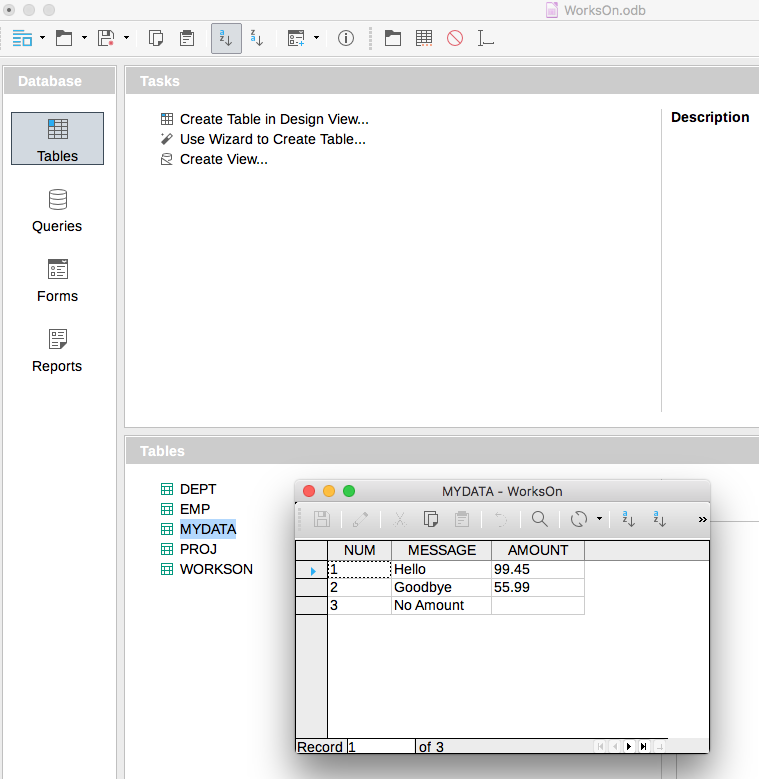
\includegraphics[width=0.9\textwidth]{img/mydataBASE}
\end{center}
\end{frame}


\begin{frame}{LibreOffice Base using lowercase letters}
To force the names of tales and fields to be lowercase in LibreOffice base, use double quotes.
\begin{center}
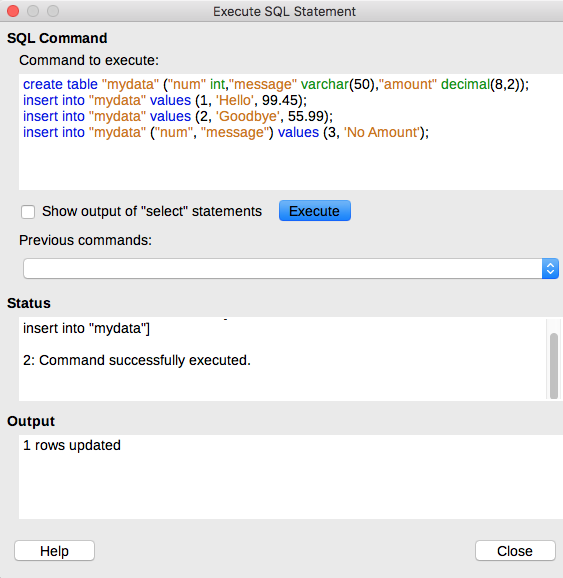
\includegraphics[width=0.45\textwidth]{img/baseLoserSQL.png} \quad
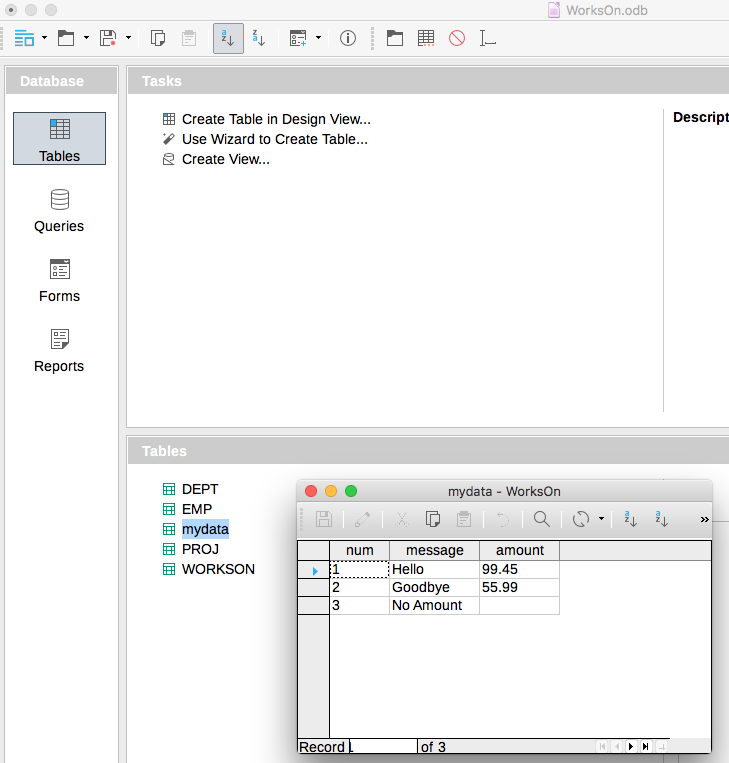
\includegraphics[width=0.45\textwidth]{img/baseLower}
\end{center}
\end{frame}


\begin{frame}{SQL view}\label{SQLaccess}
In Microsoft Access, go to the Design tab in the ribbon and select the SQL View button
\begin{center}
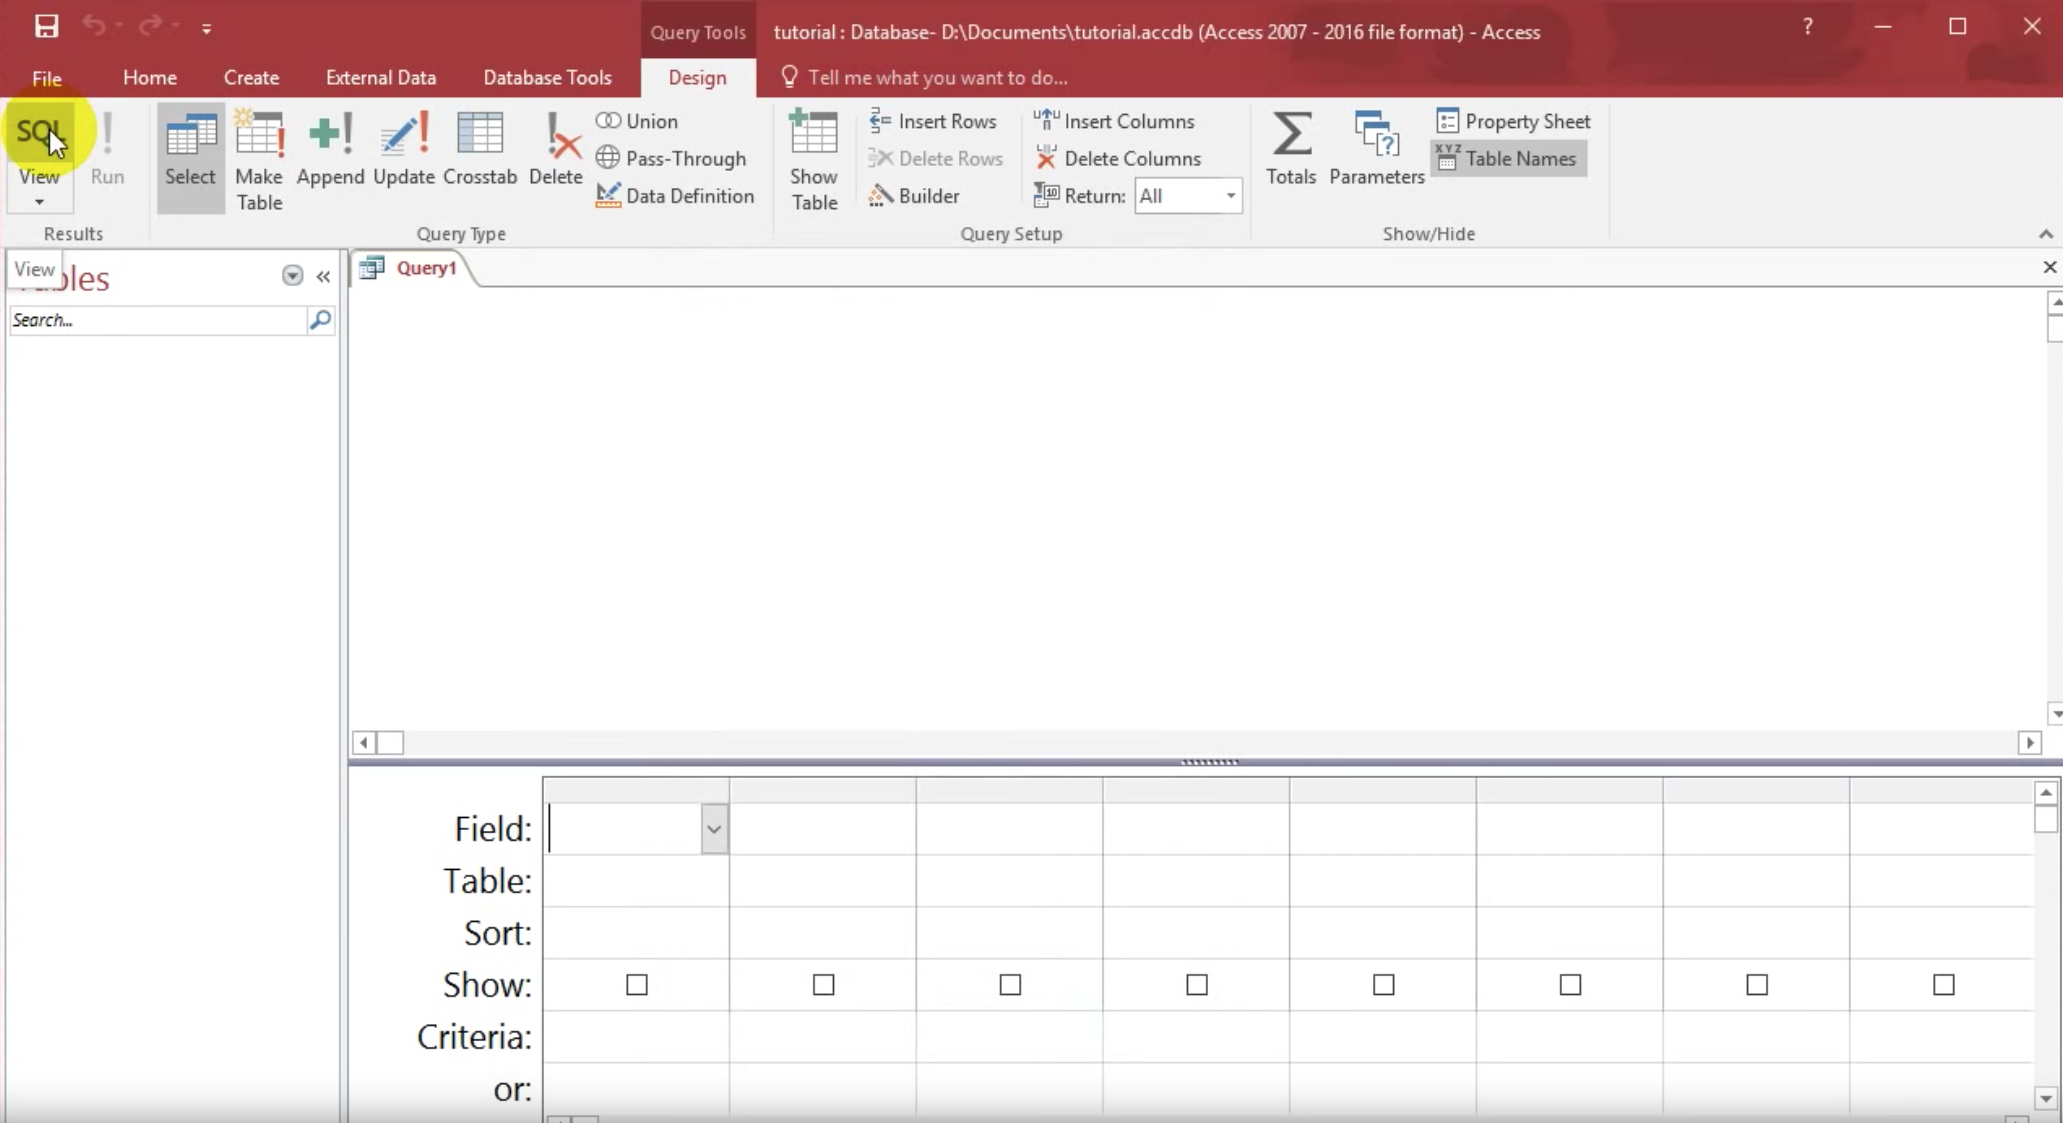
\includegraphics[width=0.9\textwidth]{img/SQLview}
\end{center}
\end{frame}


\begin{frame}{Comment}
\begin{itemize}
\item For monetary values in LibreOffice base we used the data type \command{DECIMAL}{\tt (}$x$, 2 {\tt )}.
\item For monetary values in Microsoft Access, use \command{CURRENCY} (with no arguments).
\end{itemize}
\end{frame}





\begin{frame}[fragile]
We can updating existing rows using the \command{UPDATE} statement.  Examples:
\begin{enumerate}
\item Increase all employee salaries by 10\%.
\begin{Verbatim}[frame=single, xleftmargin=1cm, xrightmargin=1cm, commandchars=\\\{\}]
\purple{UPDATE SET} salary = salary*1.10
\end{Verbatim}
\item Increase salary of employee E2 to \$1 million and change his name:
\begin{Verbatim}[frame=single, xleftmargin=1cm, xrightmargin=1cm, commandchars=\\\{\}]
\purple{UPDATE} emp 
\purple{SET} salary = 1000000, ename='Rich Guy'
\purple{WHERE} eno = 'E2';
\end{Verbatim}
\end{enumerate}

\vspace{1em}
\begin{alertblock}{INSERT vs UPDATE}
The main difference between \command{INSERT} and \command{UPDATE} is that \command{INSERT} is used to add new records to the table while \command{UPDATE} is used to modify the existing records in the table
\end{alertblock}
\end{frame}


\begin{frame}[fragile]
{\bf Notes:}
\begin{itemize}
\item Use \purple{\tt WHERE} to filter only the rows to update.
\medskip
\item The \purple{\tt WHERE} clause can also be used with other comparisons (eg. {\tt = , $>$, $<$}) with numbers, characters, or  dates.
\medskip
\item For example, you can filter on dates passed a certain time using  \verb|WHERE date > '2011-12-16'|
\begin{itemize}
\item In Access, you will need to surround your dates with \verb|#|, eg \verb|WHERE date > #2011-12-16#|
\medskip
\end{itemize}
\item Notice how we can also change (i.e \purple{\tt SET}) more than one value at a time by separating the fields by commas.
\medskip
\item Notice that there are no commas separating keyword clauses
\medskip

\end{itemize}



\end{frame}


\frame{
\ft{Updating in Microsoft Access and LibreOffice Base}
The \command{UPDATE} command is  supported by Microsoft Access/LibreOffice Base's GUI. That is, to modify individual data items with SQL code, simply enter the table, select the row and cell to update and change the data.  Data is saved when you leave the row.
\begin{center}
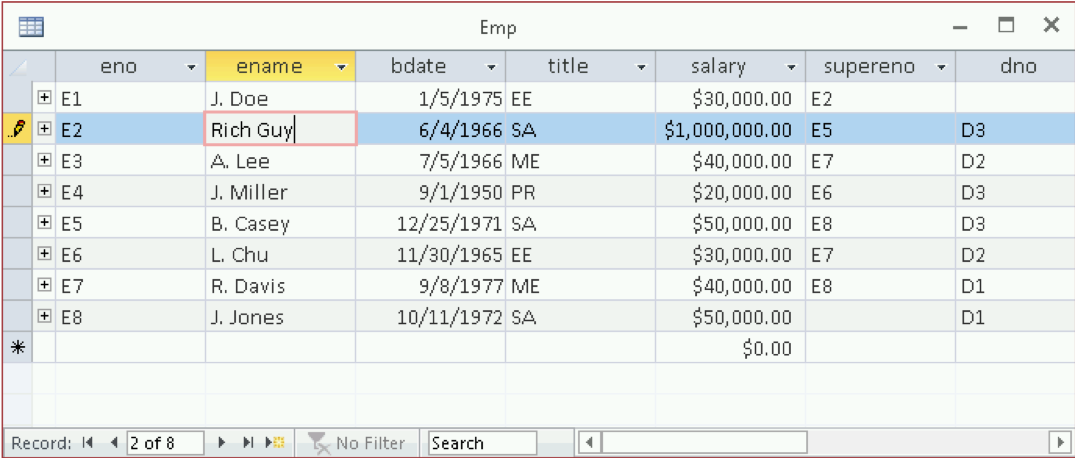
\includegraphics[width=0.9\textwidth]{img/update}
\end{center}

}

\frame{
\begin{example}
{Question} Using the {\tt mydata} table and the three rows previously inserted do these updates:
\begin{itemize}
\item Update all {\tt amount} fields to be 99.99.
\item Update the {\tt num} field and set it to 10 for the record with {\tt num = 1}.
\item Update the message field to 'Changed' for the record with {\tt num = 2}.
\end{itemize}

Perform these takes in SQL mode in either Access, Base, or sqlfiddle.com.
%To use SQL commands rather than Design View, go to {\bf Tools} $>$ {\bf SQL}.
\end{example}
}

\frame{
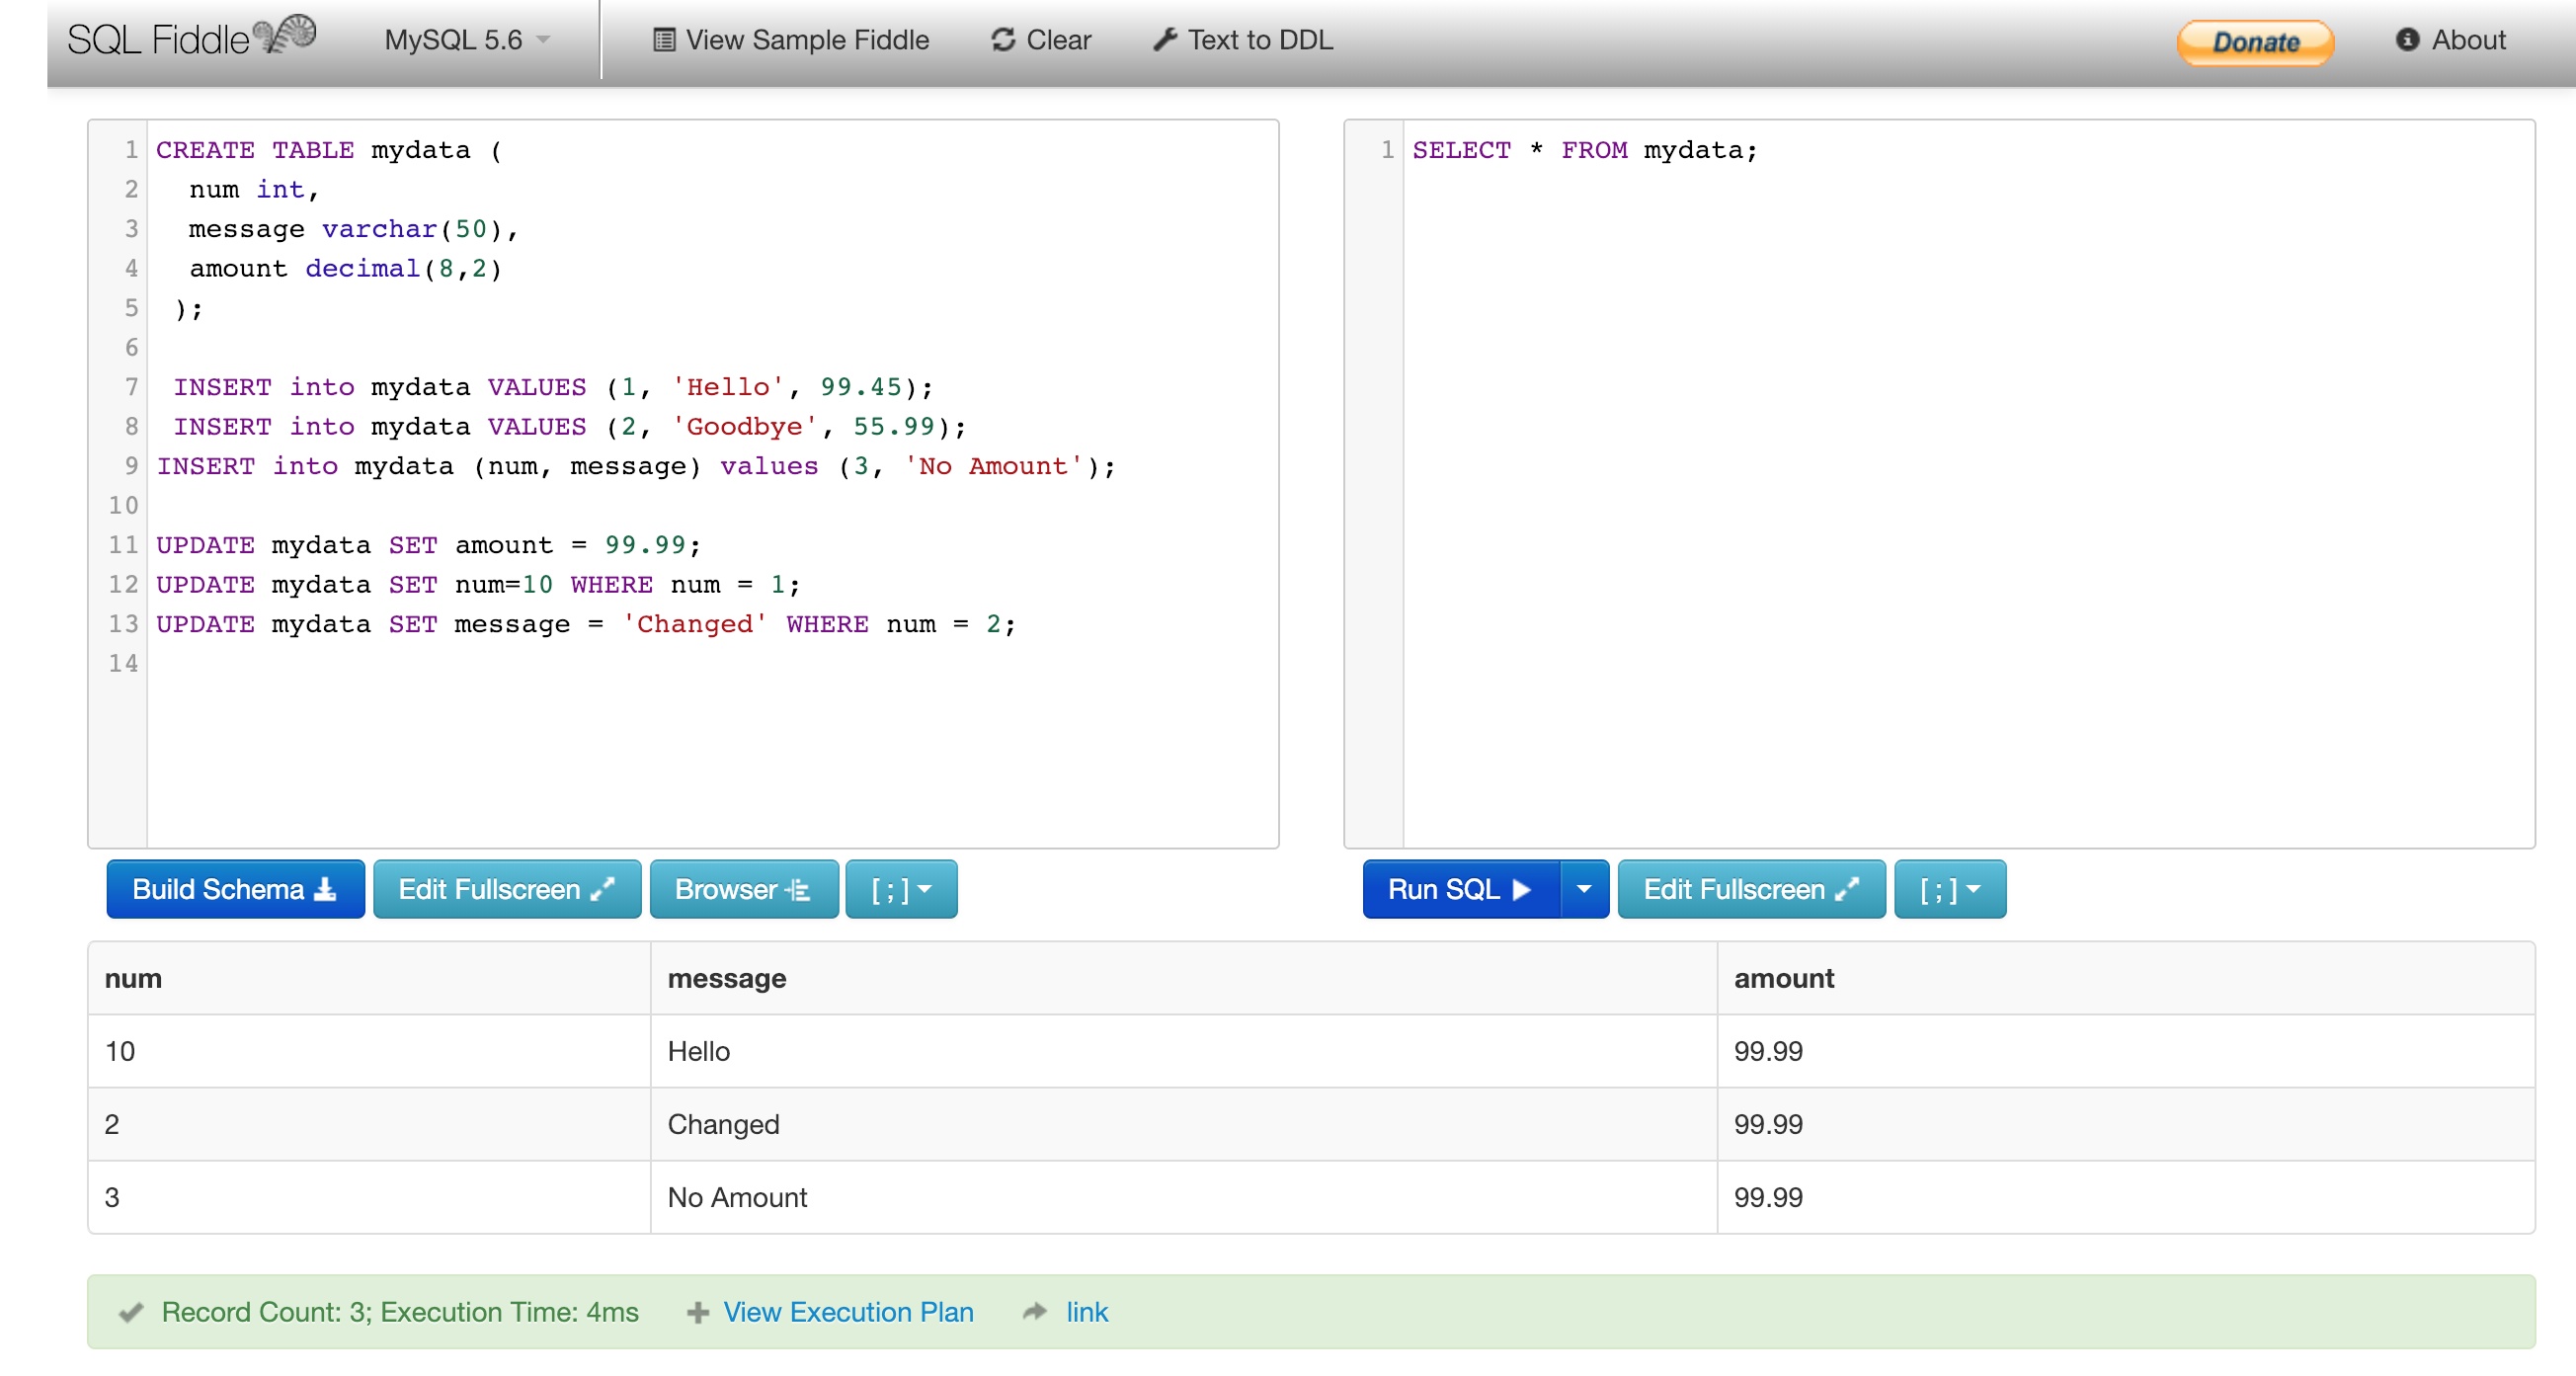
\includegraphics[width=1\textwidth]{img/SQLfiddle2.png}\\
}



\begin{frame}[fragile]{Adding/Deleting Attributes}
We can add or delete \textit{columns}  using the \command{ALTER} statement.  
\vfill
\begin{enumerate}
\item To add the column {\tt notes} to our {\tt emp} table:\\
\begin{Verbatim}[commandchars=\\\{\}, xleftmargin=0.1in, frame=single]
\purple{ALTER TABLE} emp 
\purple{ADD COLUMN} notes VARCHAR(50);
\end{Verbatim}
\vspace{1em}

Alternatively we could just type \command{ADD}:
\begin{Verbatim}[commandchars=\\\{\}, xleftmargin=0.1in, frame=single]
\purple{ALTER TABLE}  emp 
\purple{ADD} notes VARCHAR(50);
\end{Verbatim}
\vfill

\item To delete the column {\tt notes} from our {\tt emp} table:\\
\begin{Verbatim}[commandchars=\\\{\}, xleftmargin=0.1in, frame=single]
\purple{ALTER TABLE} emp
\purple{DROP COLUMN} notes;
\end{Verbatim}
\vfill
\end{enumerate}
\end{frame}

\begin{frame}{Adding/Deleting Attributes}
{\bf Notes:}
\begin{itemize}
\item Note that we don't need quotes for field names (just as we didn't need them in the \command{CREATE TABLE} statement).
\item We can not at a column at a specific position in the table (they get placed in the last row by default).
\item We can add multiple columns at a time using the syntax:\\
\command{ALTER TABLE} {\tt table\_name} \\
  {\tt \purple{ADD}  column\_1 column\_definition, column\_2 column\_definition};
\end{itemize}
\end{frame}



\frame{
\ft{Delete Statements}
Rows are deleted using the \command{DELETE} statement. Examples:
\begin{itemize}
\item Fire everyone in the company.\\
\quad {\tt \purple{DELETE FROM }emp;}
\item Fire everyone making over \$35,000.\\
 \quad {\tt \purple{DELETE FROM} emp \purple{      WHERE} salary > 35000;}
\item You can think of the previous example as deleting all the visible rows in an excel sheet after applying a filter.
\end{itemize}

}


\frame{
\ft{Deleting Data in Microsoft Access/LibreOffice Base}
The \command{DELETE} command is supported by Microsoft Access/LibreOffice Base GUI. To delete an individual row, select the row (by clicking the gray space to the left of the row), then press \keystroke{Alt}+\keystroke{Delete} key or right click and select {\bf Delete Row} from pop-up menu.\footnote{I sometimes get weird errors when trying to use this feature}
  \begin{center}
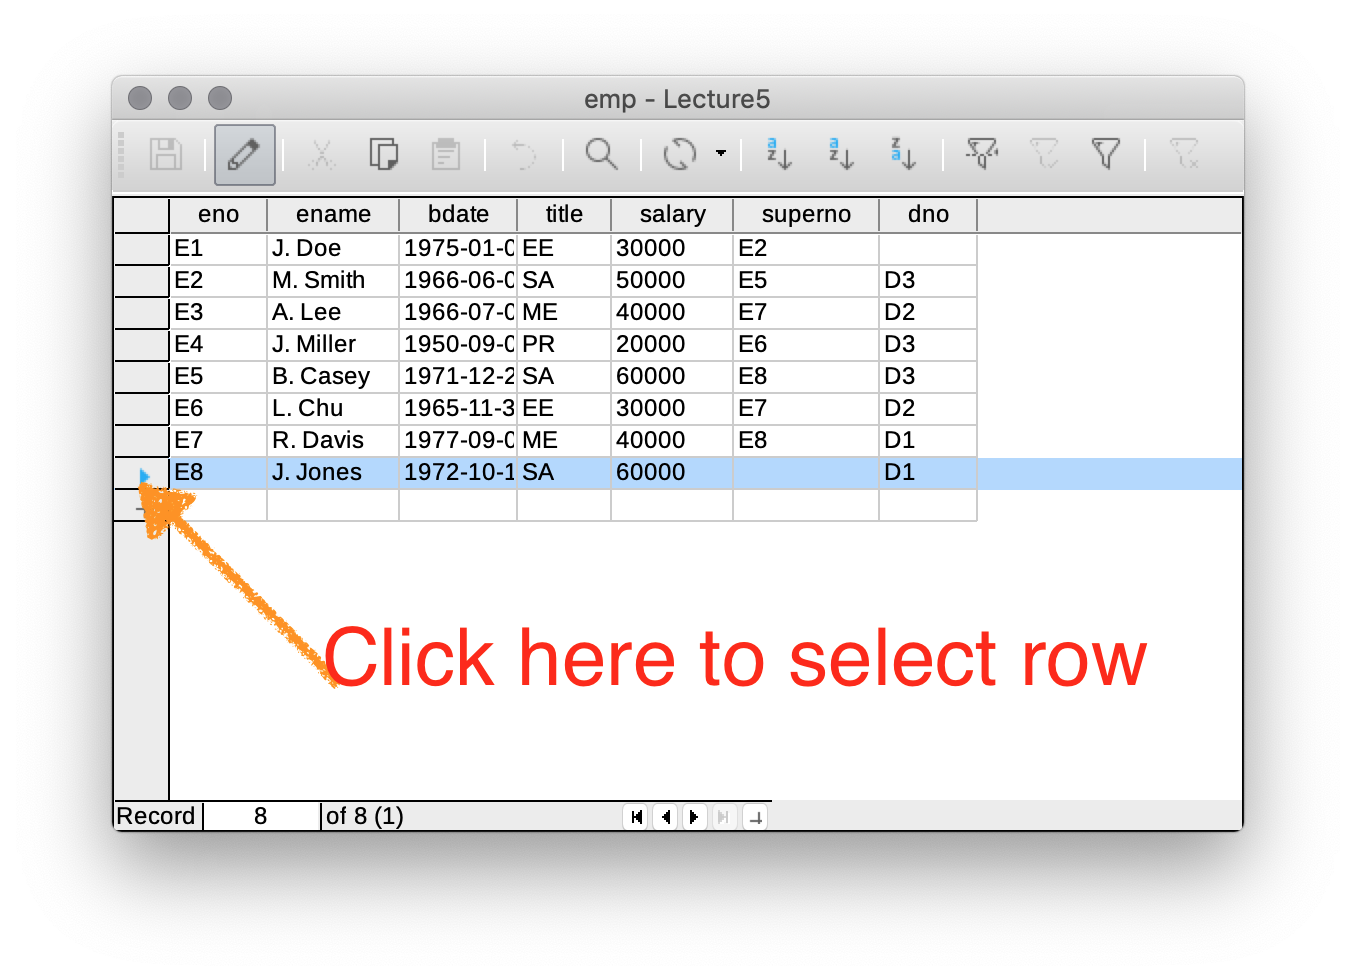
\includegraphics[width=0.6\textwidth]{img/deleteRow}
\end{center}

}

\frame{
\ft{Deleting Data in Microsoft Access/LibreOffice Base}
The \command{DELETE} command is supported by Microsoft Access/LibreOffice Base. To delete an individual row, select the row (by clicking the gray space to the left of the row), then press \keystroke{Delete} key or right click select {\bf Delete Record} from pop-up menu.
  \begin{center}
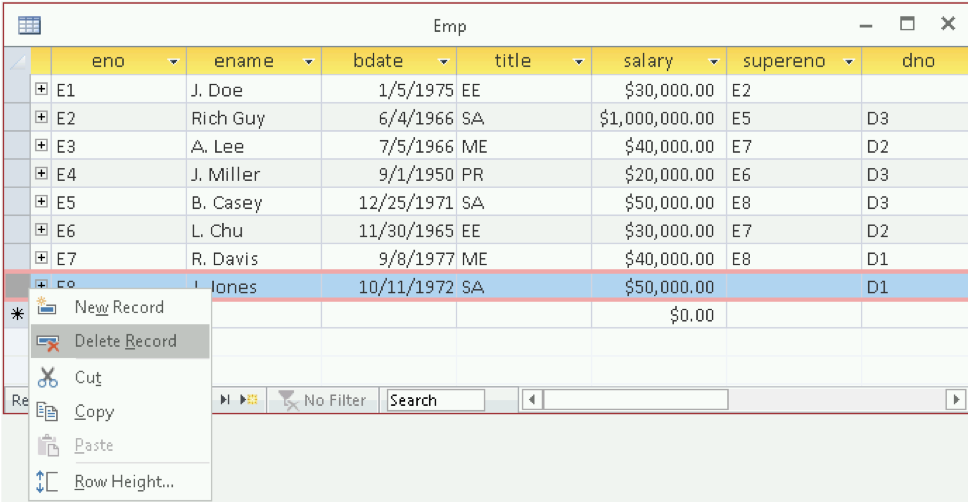
\includegraphics[width=0.9\textwidth]{img/delete}
\end{center}

}





\frame{
\begin{example}
[Delete] Using the {\tt mydata} table and the three rows previously inserted do these deletes:
\begin{itemize}
\item Delete the row with num = 10.
\item Delete the row(s) with message > 'D'.
\item Delete all rows.
\end{itemize}
You can use Access, LibreOffice Base, or sqlfiddle.com.
\end{example}
}


\frame{
Let's have a look at the current table {\tt mydata}
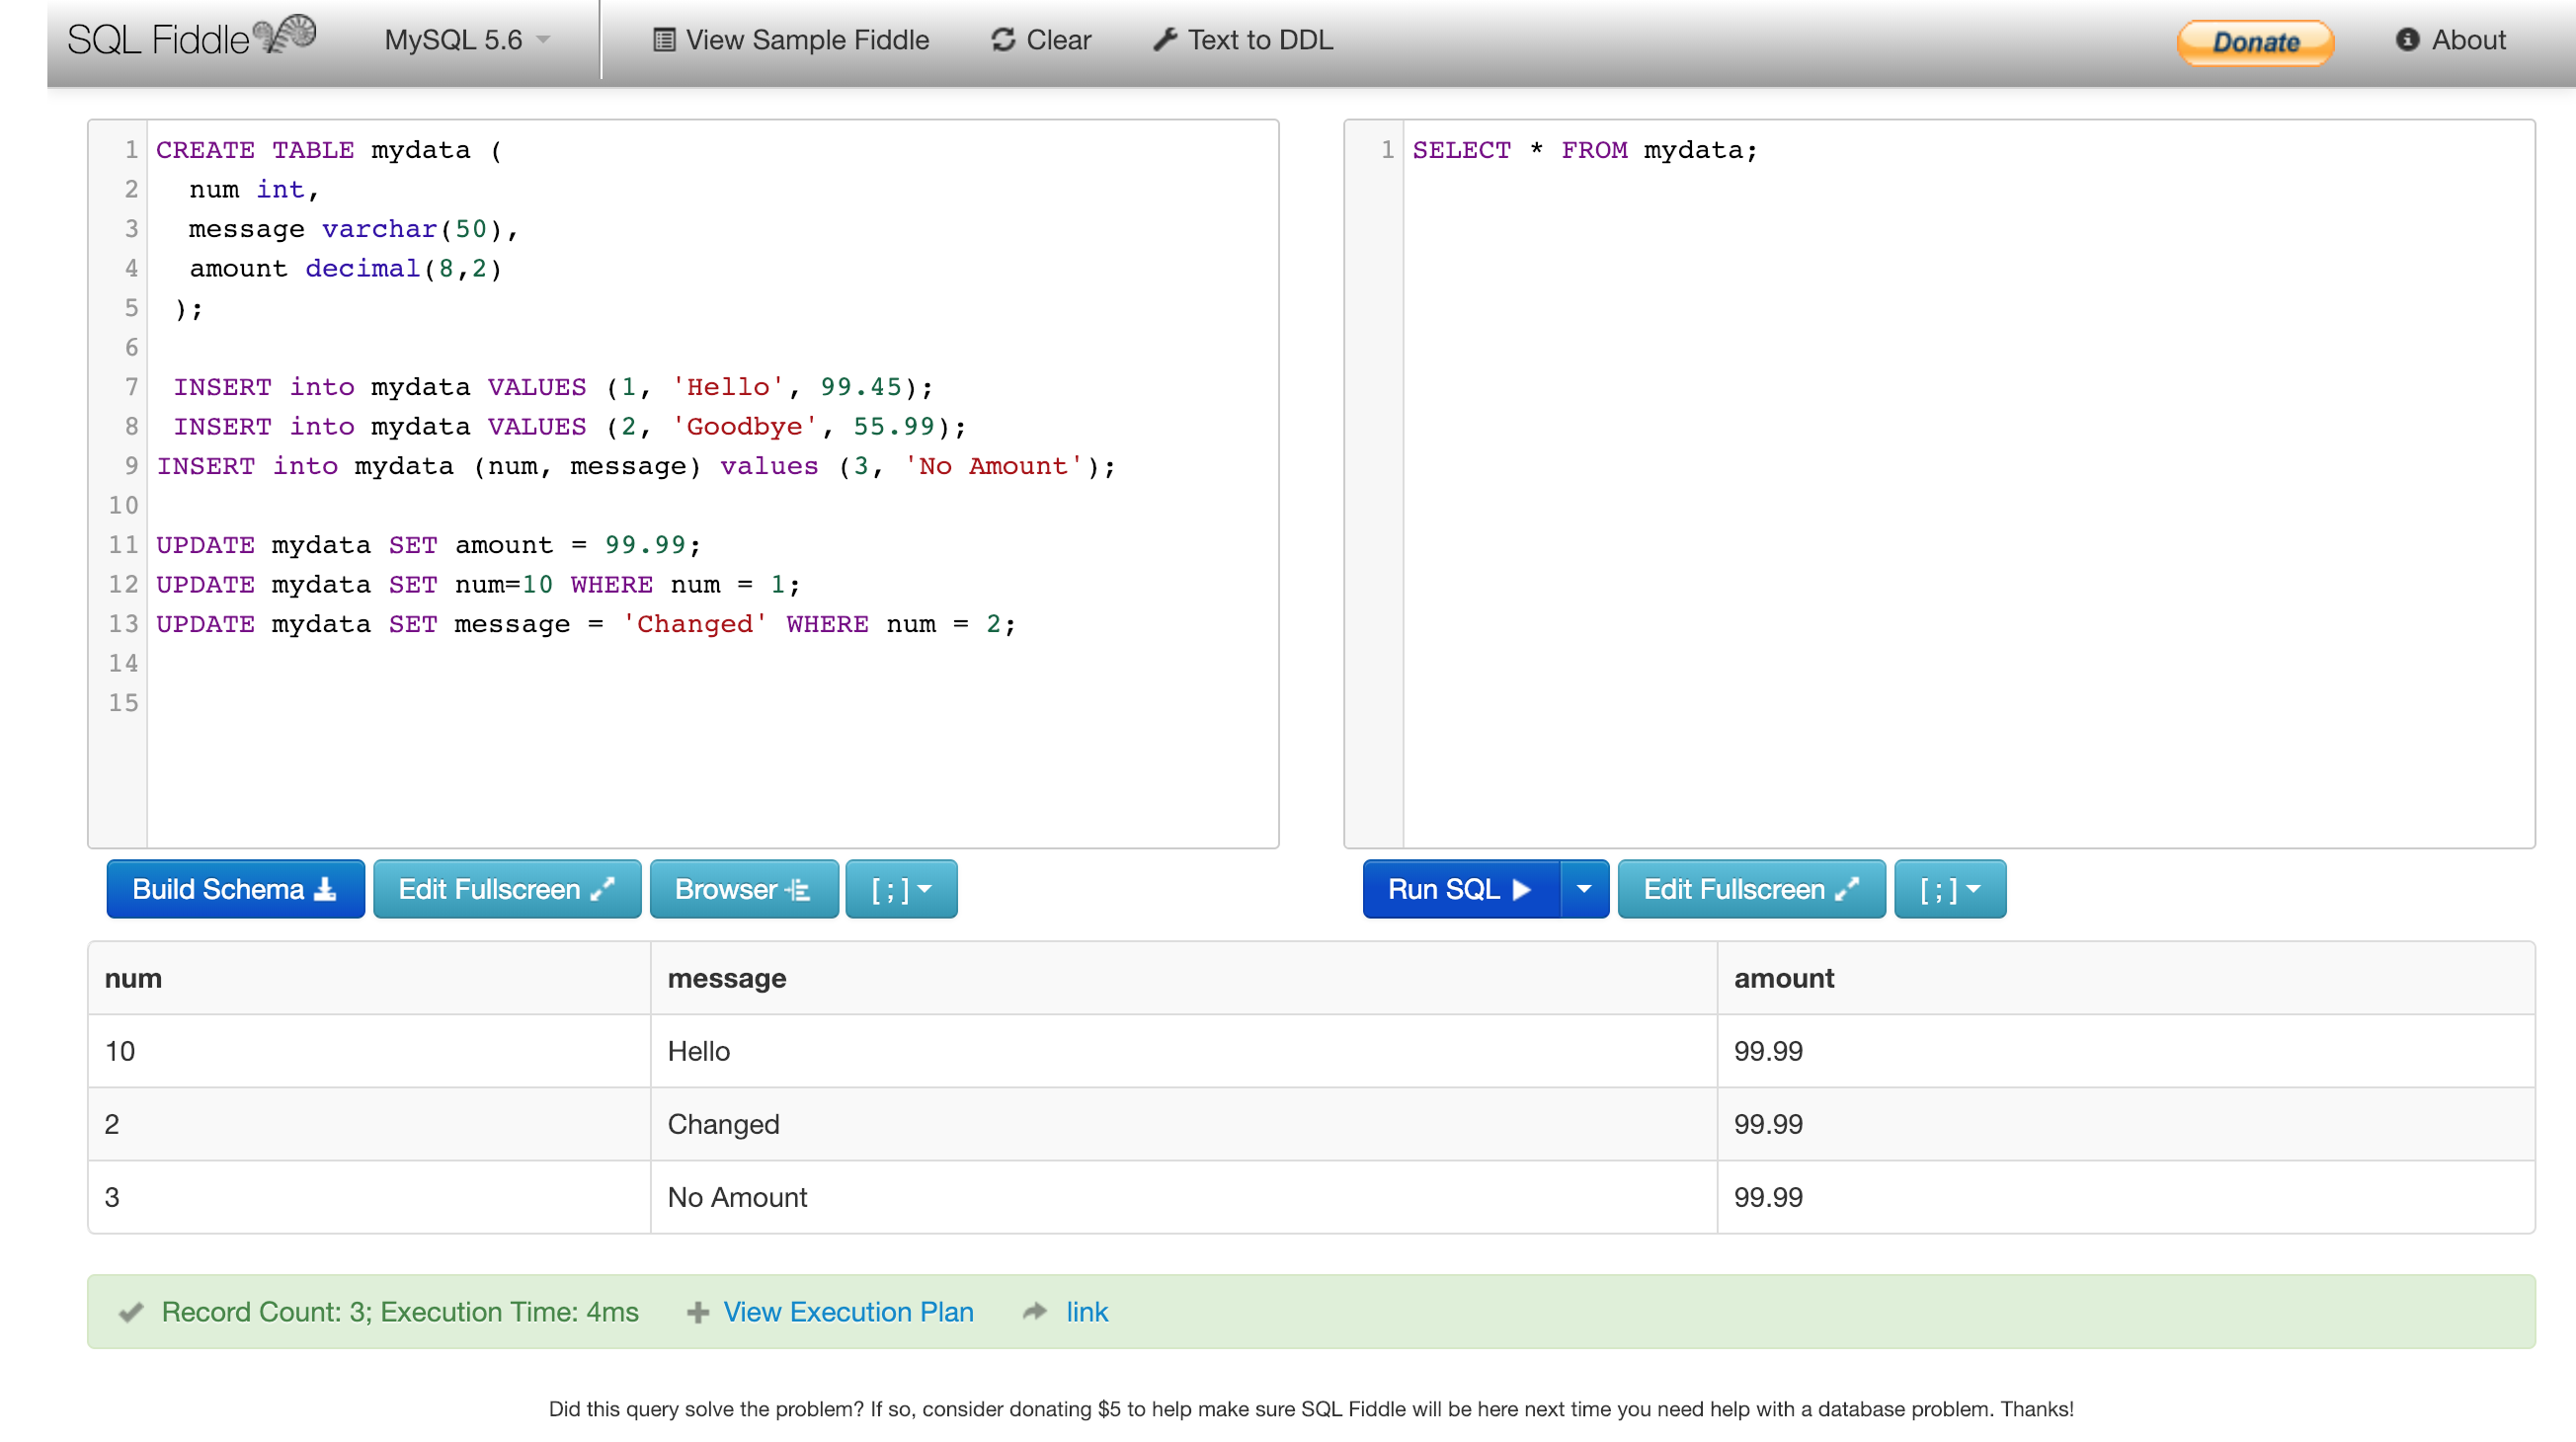
\includegraphics[width=1.2\textwidth]{img/mydataRaw}

}

\frame{
\ft{ Delete the row with {\tt num = 10}}
{\tt \purple{DELTE FROM} mydata \purple{WHERE}  num = 10;}
  \begin{center}
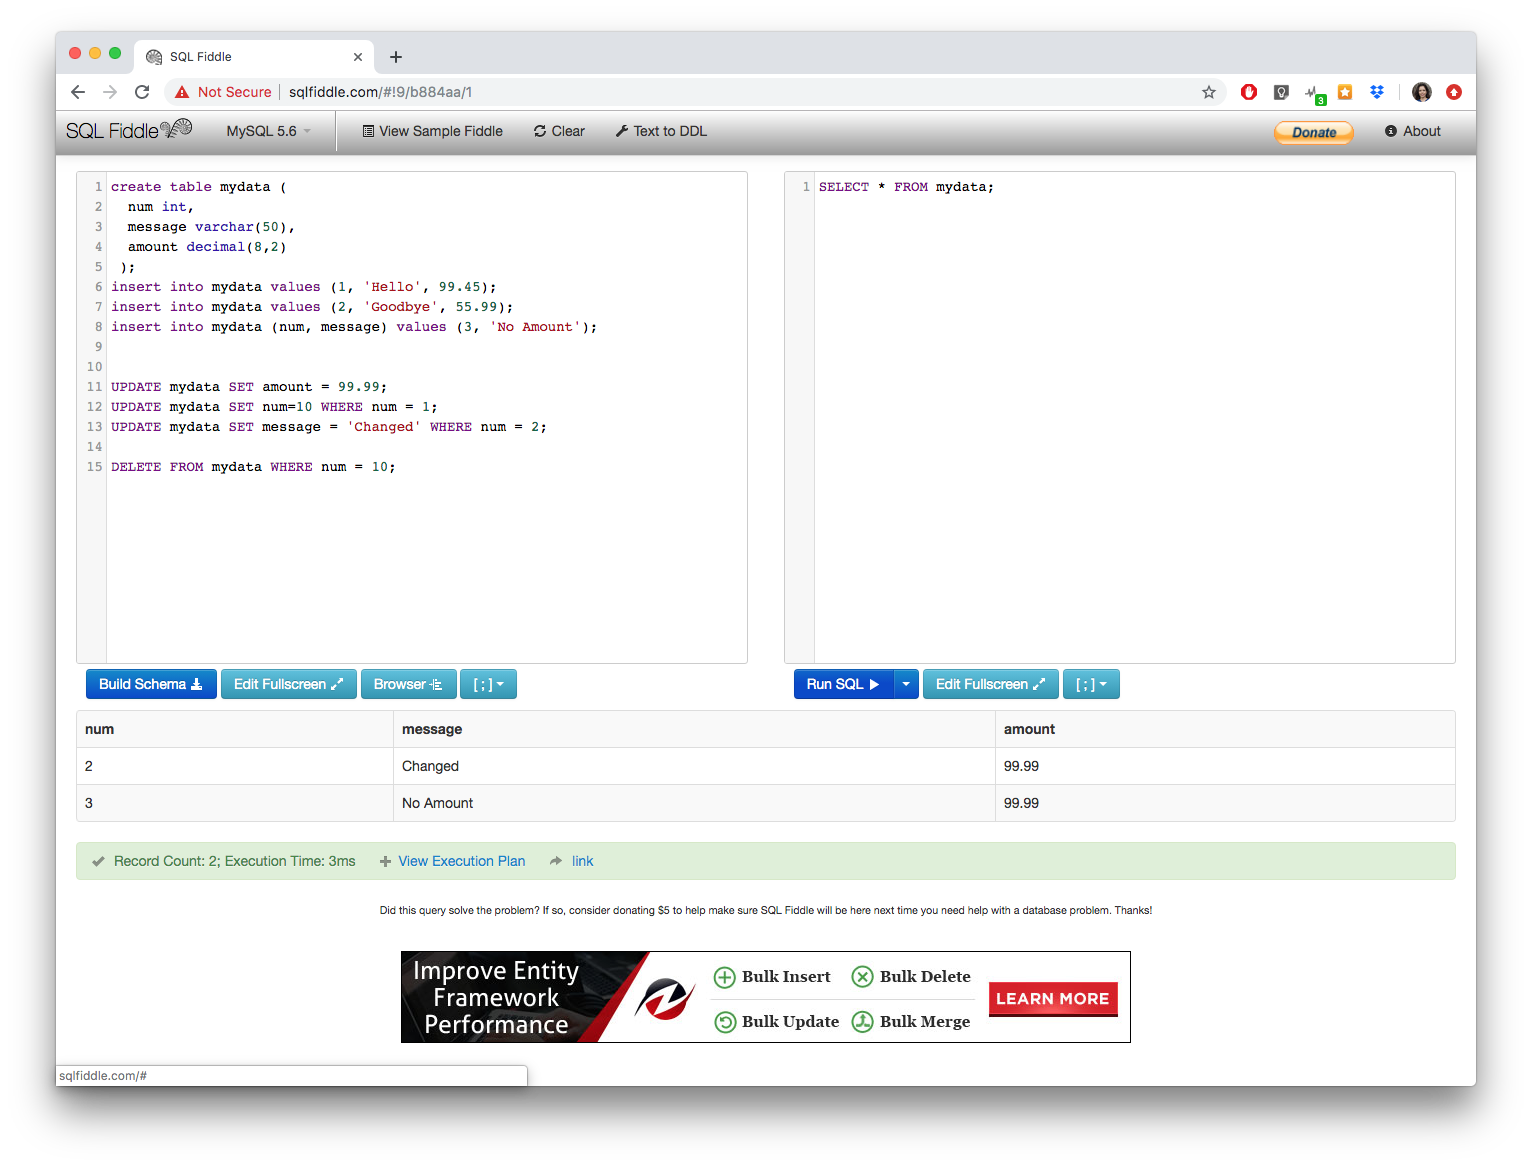
\includegraphics[width=0.99\textwidth]{img/delete10.png}
\end{center}
}


\frame{
\ft{ Delete the row(s) with message > 'D'.}
Let's look at what {\tt > 'D'} looks like anyhow:
  \begin{center}
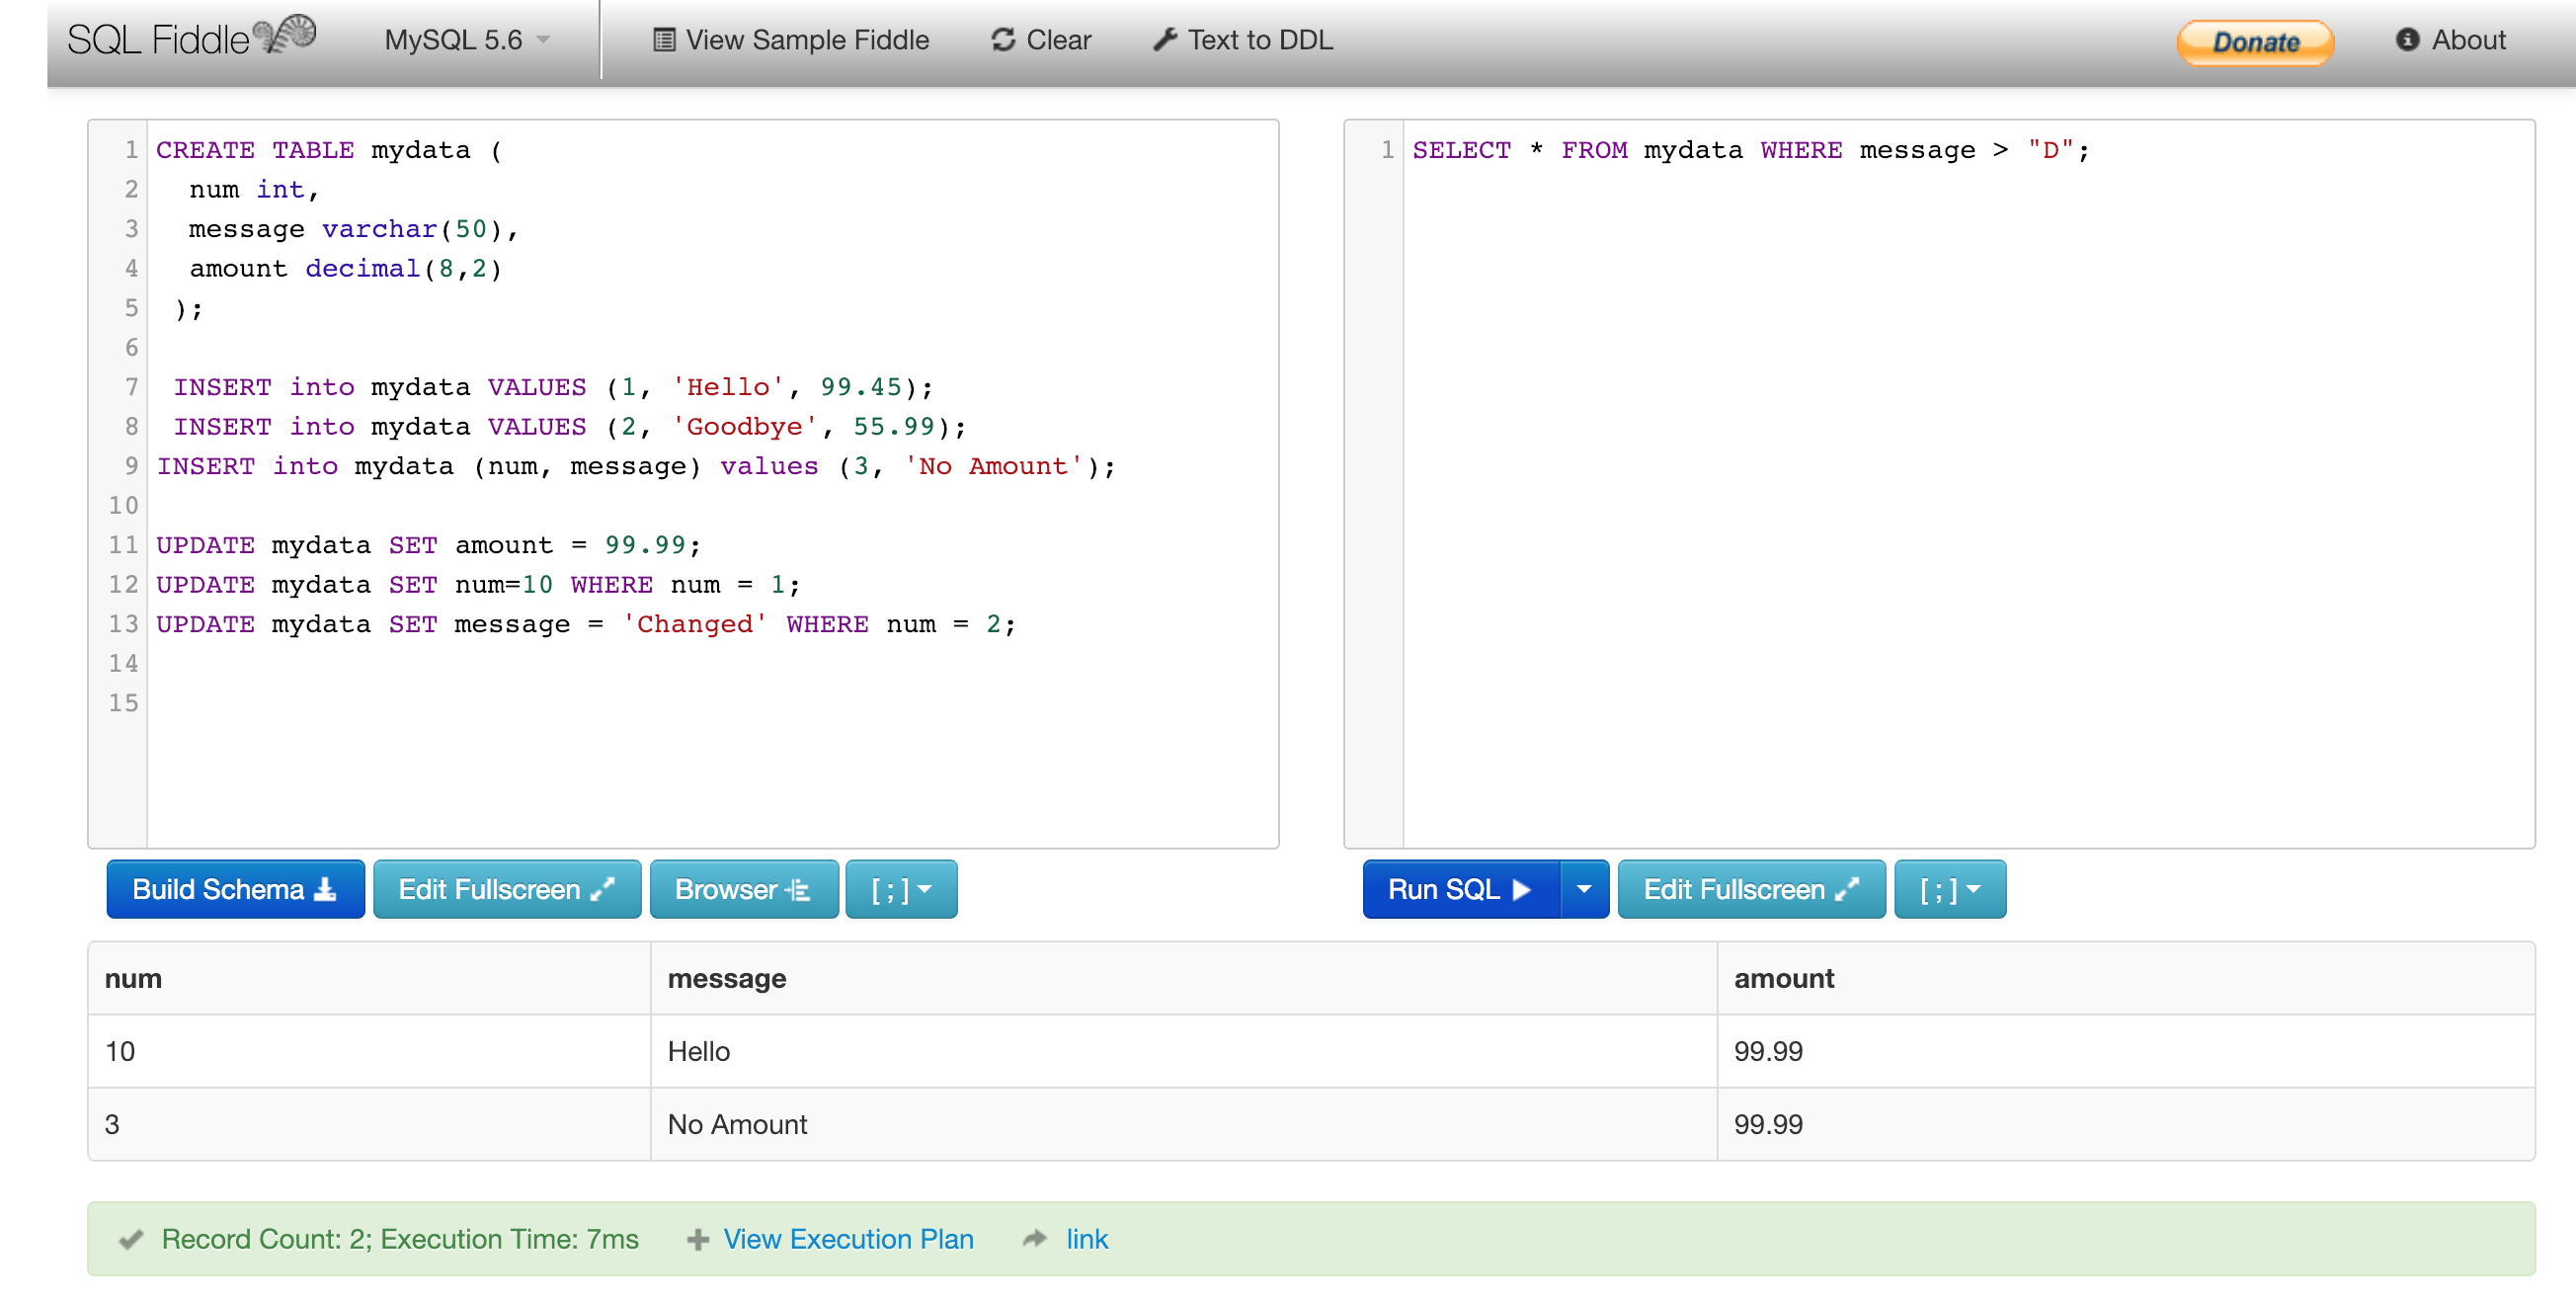
\includegraphics[width=0.99\textwidth]{img/mydataGd}
\end{center}
}


\frame{
\ft{ Delete the row(s) with message > 'D'.}
So removing the rows greater than D yeilds:
  \begin{center}
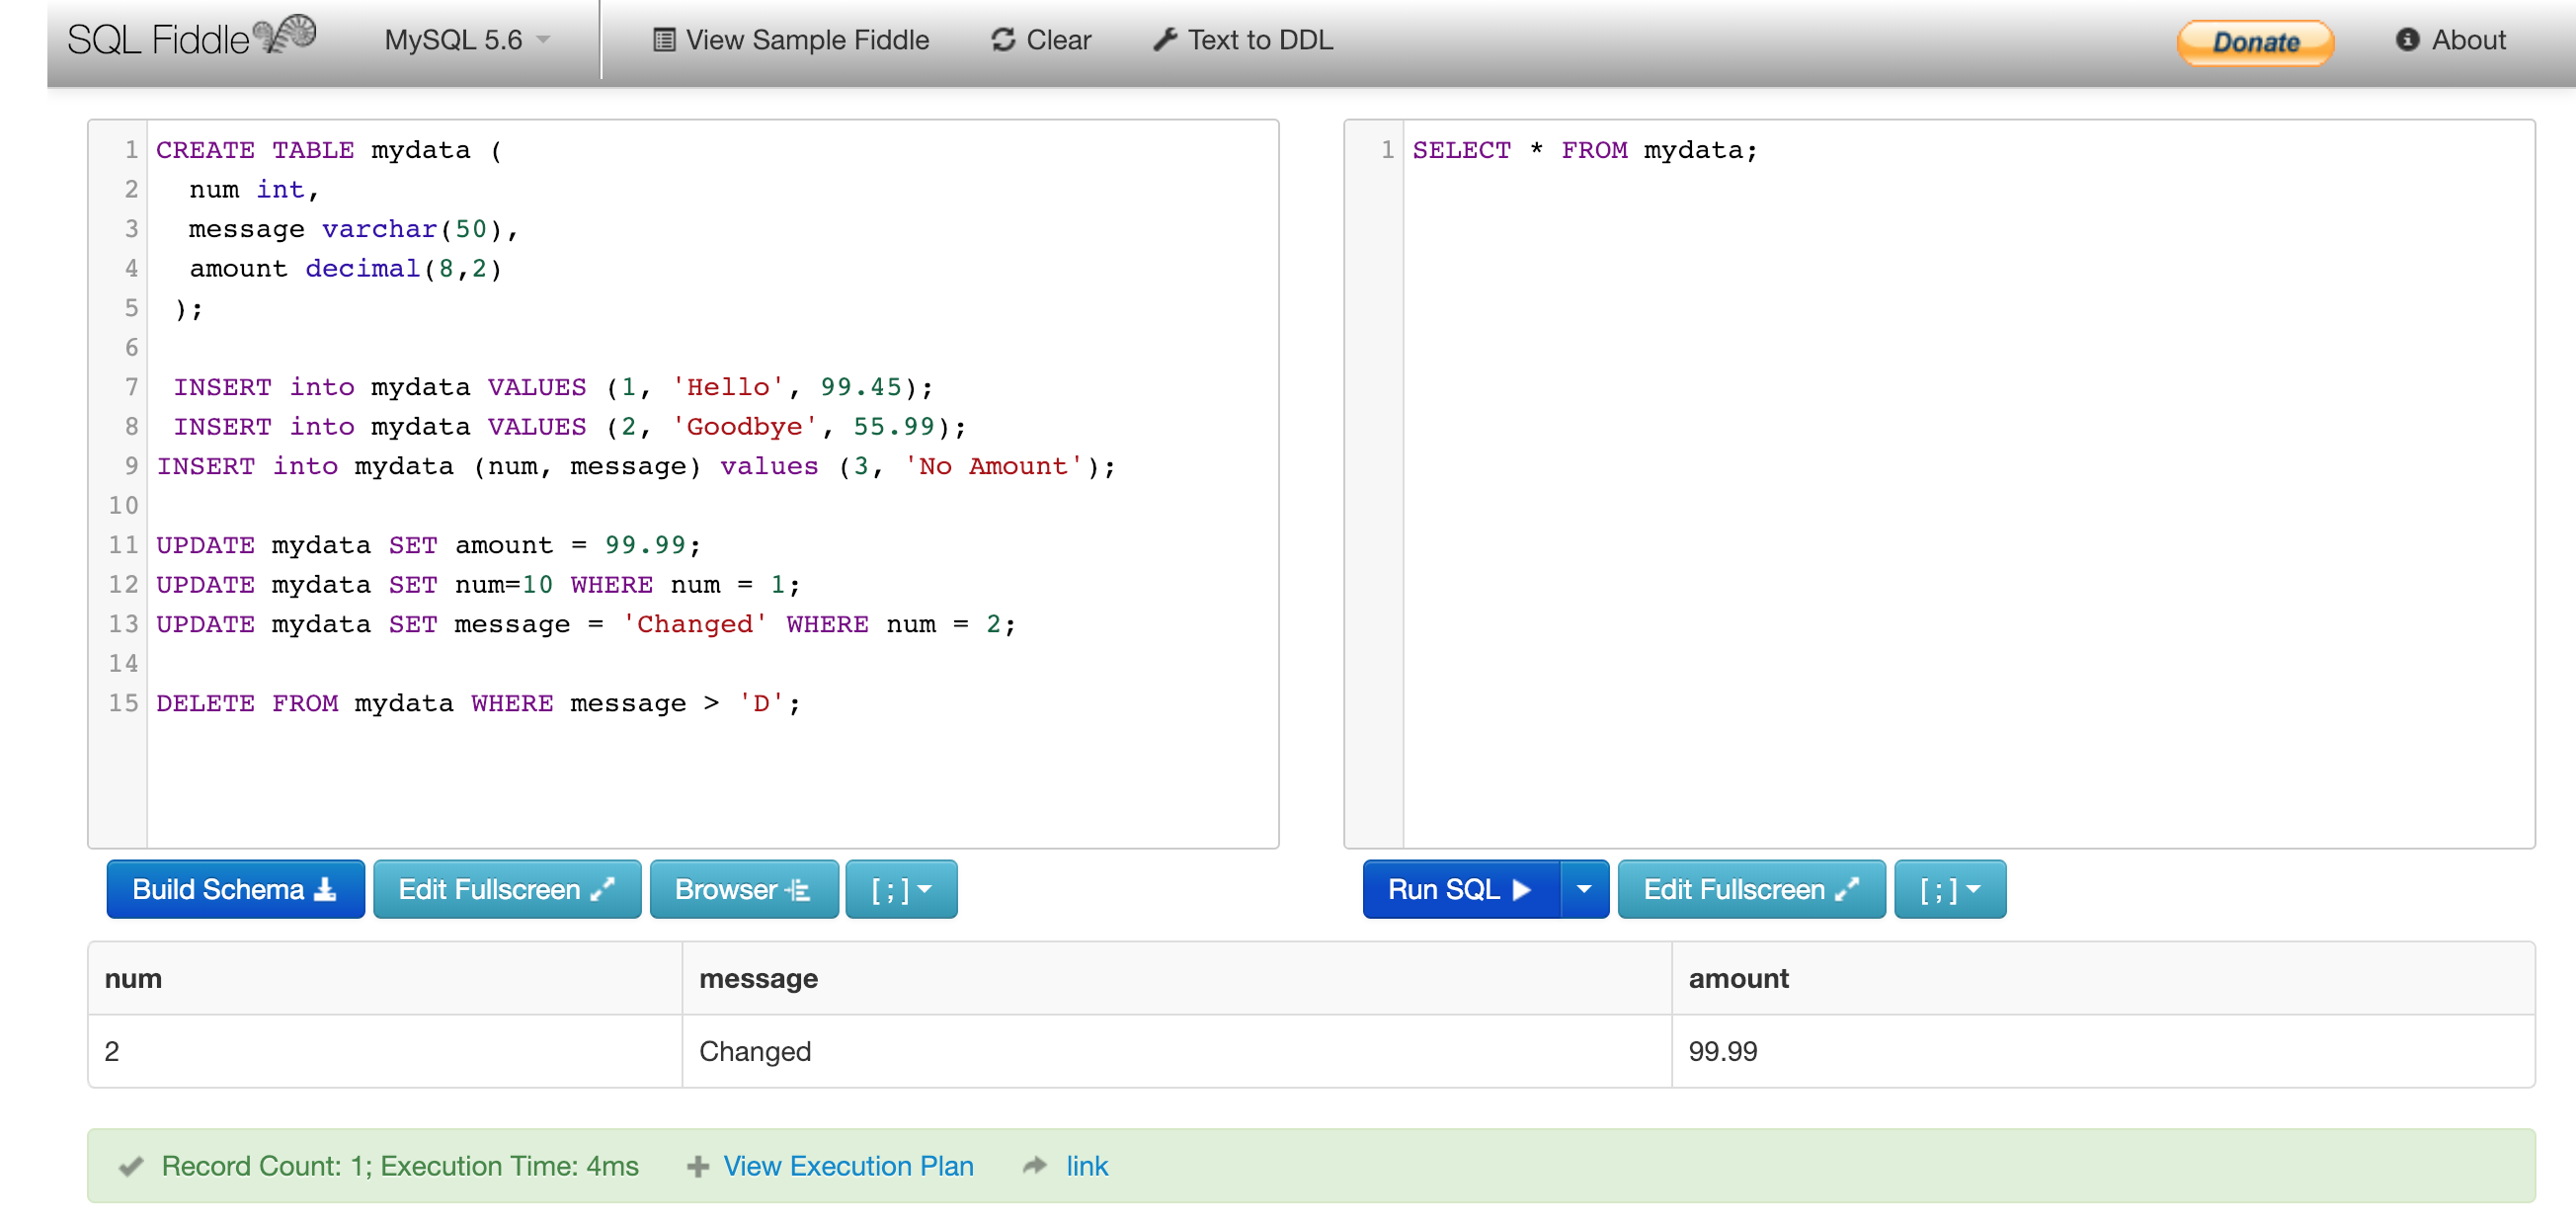
\includegraphics[width=0.99\textwidth]{img/rmD}
\end{center}
}

%\frame{  \begin{center}
%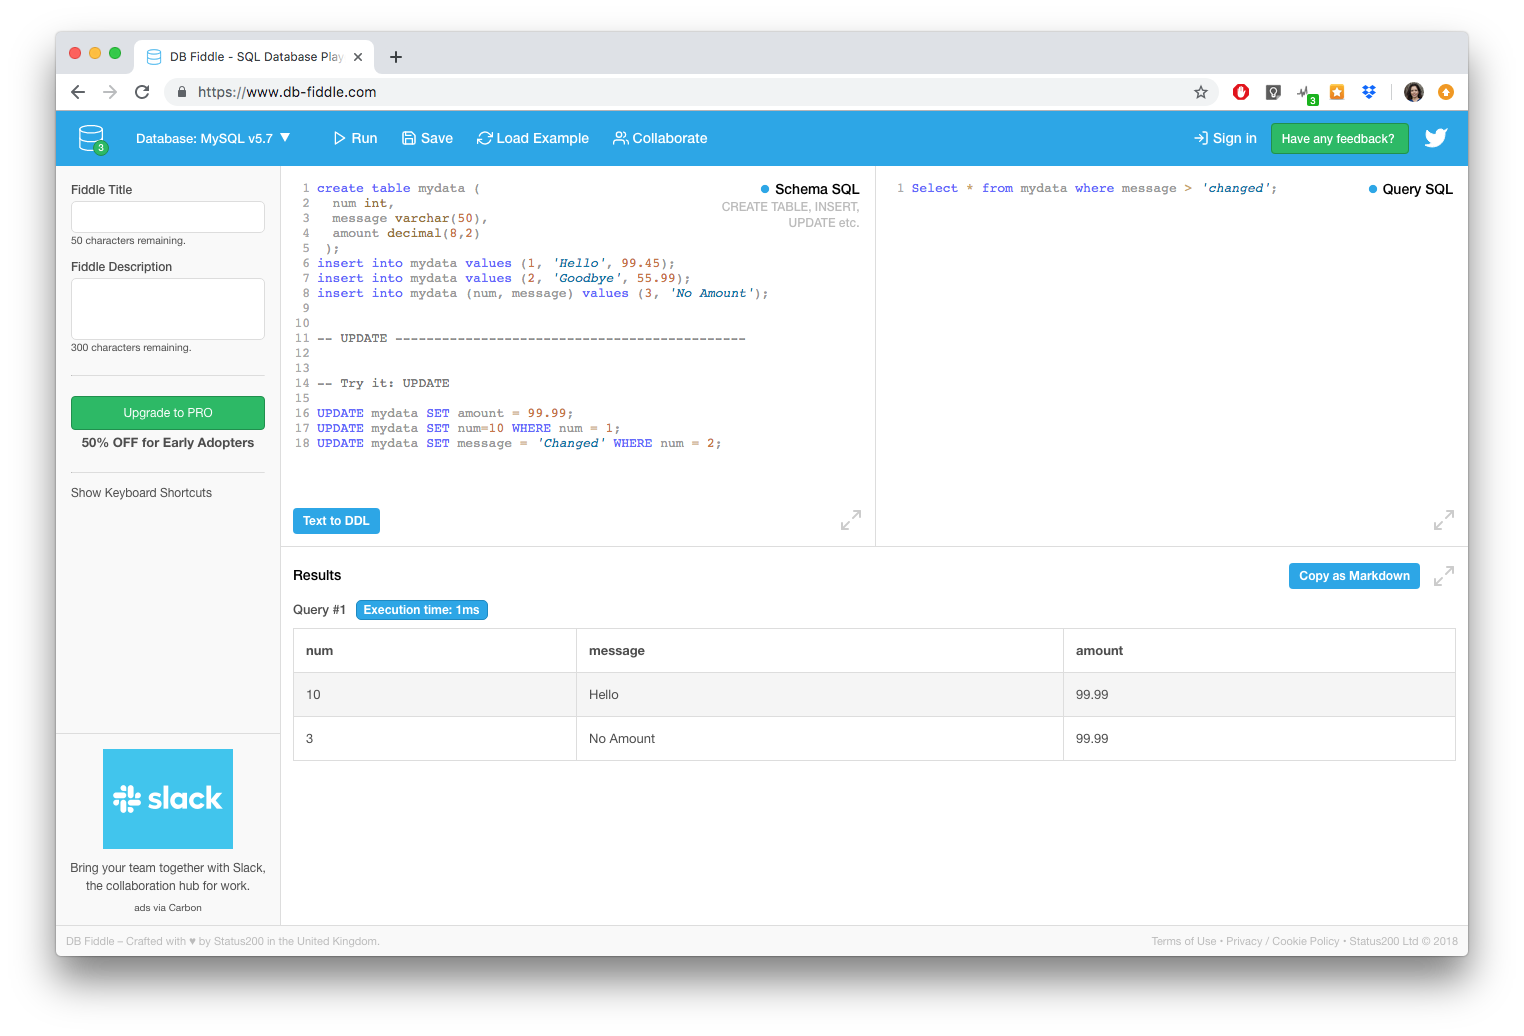
\includegraphics[width=0.99\textwidth]{img/dbfiddle}
%\end{center}
%}



\frame{
\ft{Comparison operators on strings}
\begin{itemize}
\item Comparison operators on strings uses \href{https://en.wikipedia.org/wiki/Lexicographical_order}{lexicographical ordering}.
\vfill
\item \red{Warning:}  This is similar to the alphabetical order  except \red{sometimes} all the lowercase letters come before all the uppercase letters and other times  all the uppercase letters come before all the lowercase letters.
\end{itemize}
%  \begin{center}
%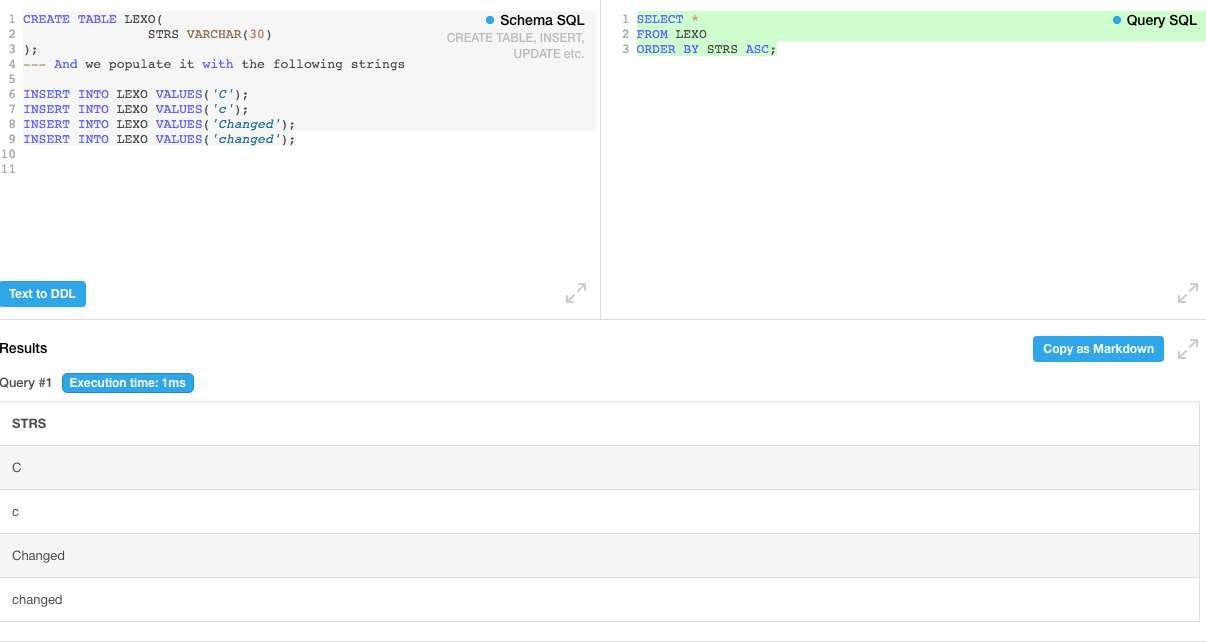
\includegraphics[width=0.99\textwidth]{img/lexo1}
%\end{center}
}



\frame{
\ft{Comparison operators on strings }
On DB-fiddle $C < c < Changed < change$ % WRONG
 in lexicographical order, hence: 

  \begin{center}
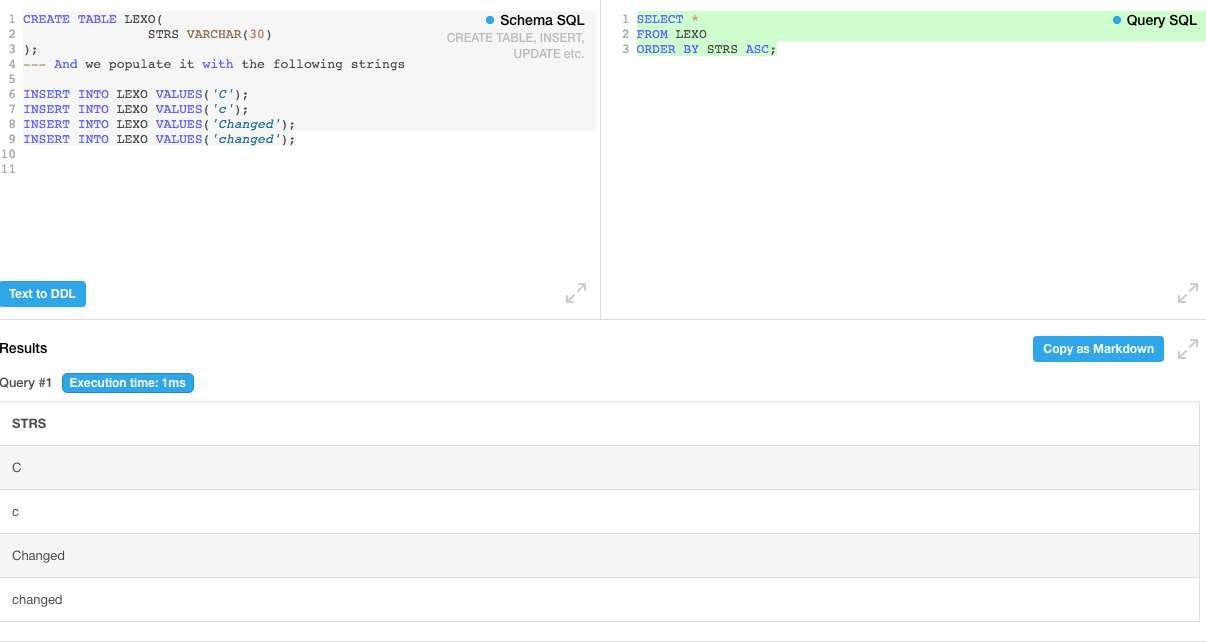
\includegraphics[width=0.99\textwidth]{img/lexo1}
\end{center}
}



\frame{
\ft{Comparison operators on strings}
On LibreOffice Base $c < C < changed < Changed$
%$C < c < Changed < change$ % WRONG
 in lexicographical order, hence: 

  \begin{center}
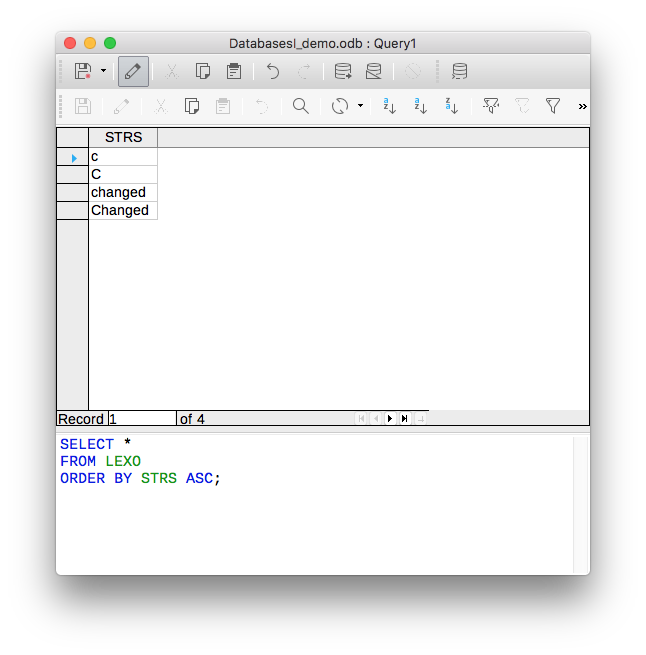
\includegraphics[width=0.99\textwidth]{img/lexo2}
\end{center}
}

%
%\frame{
%\ft{ A warning when using comparison operators.}
%\begin{alertblock}{Warning}
%Using $>$ on letters gets treated as $\geq$ in SQLfiddle.
%\end{alertblock}
%  \begin{center}
%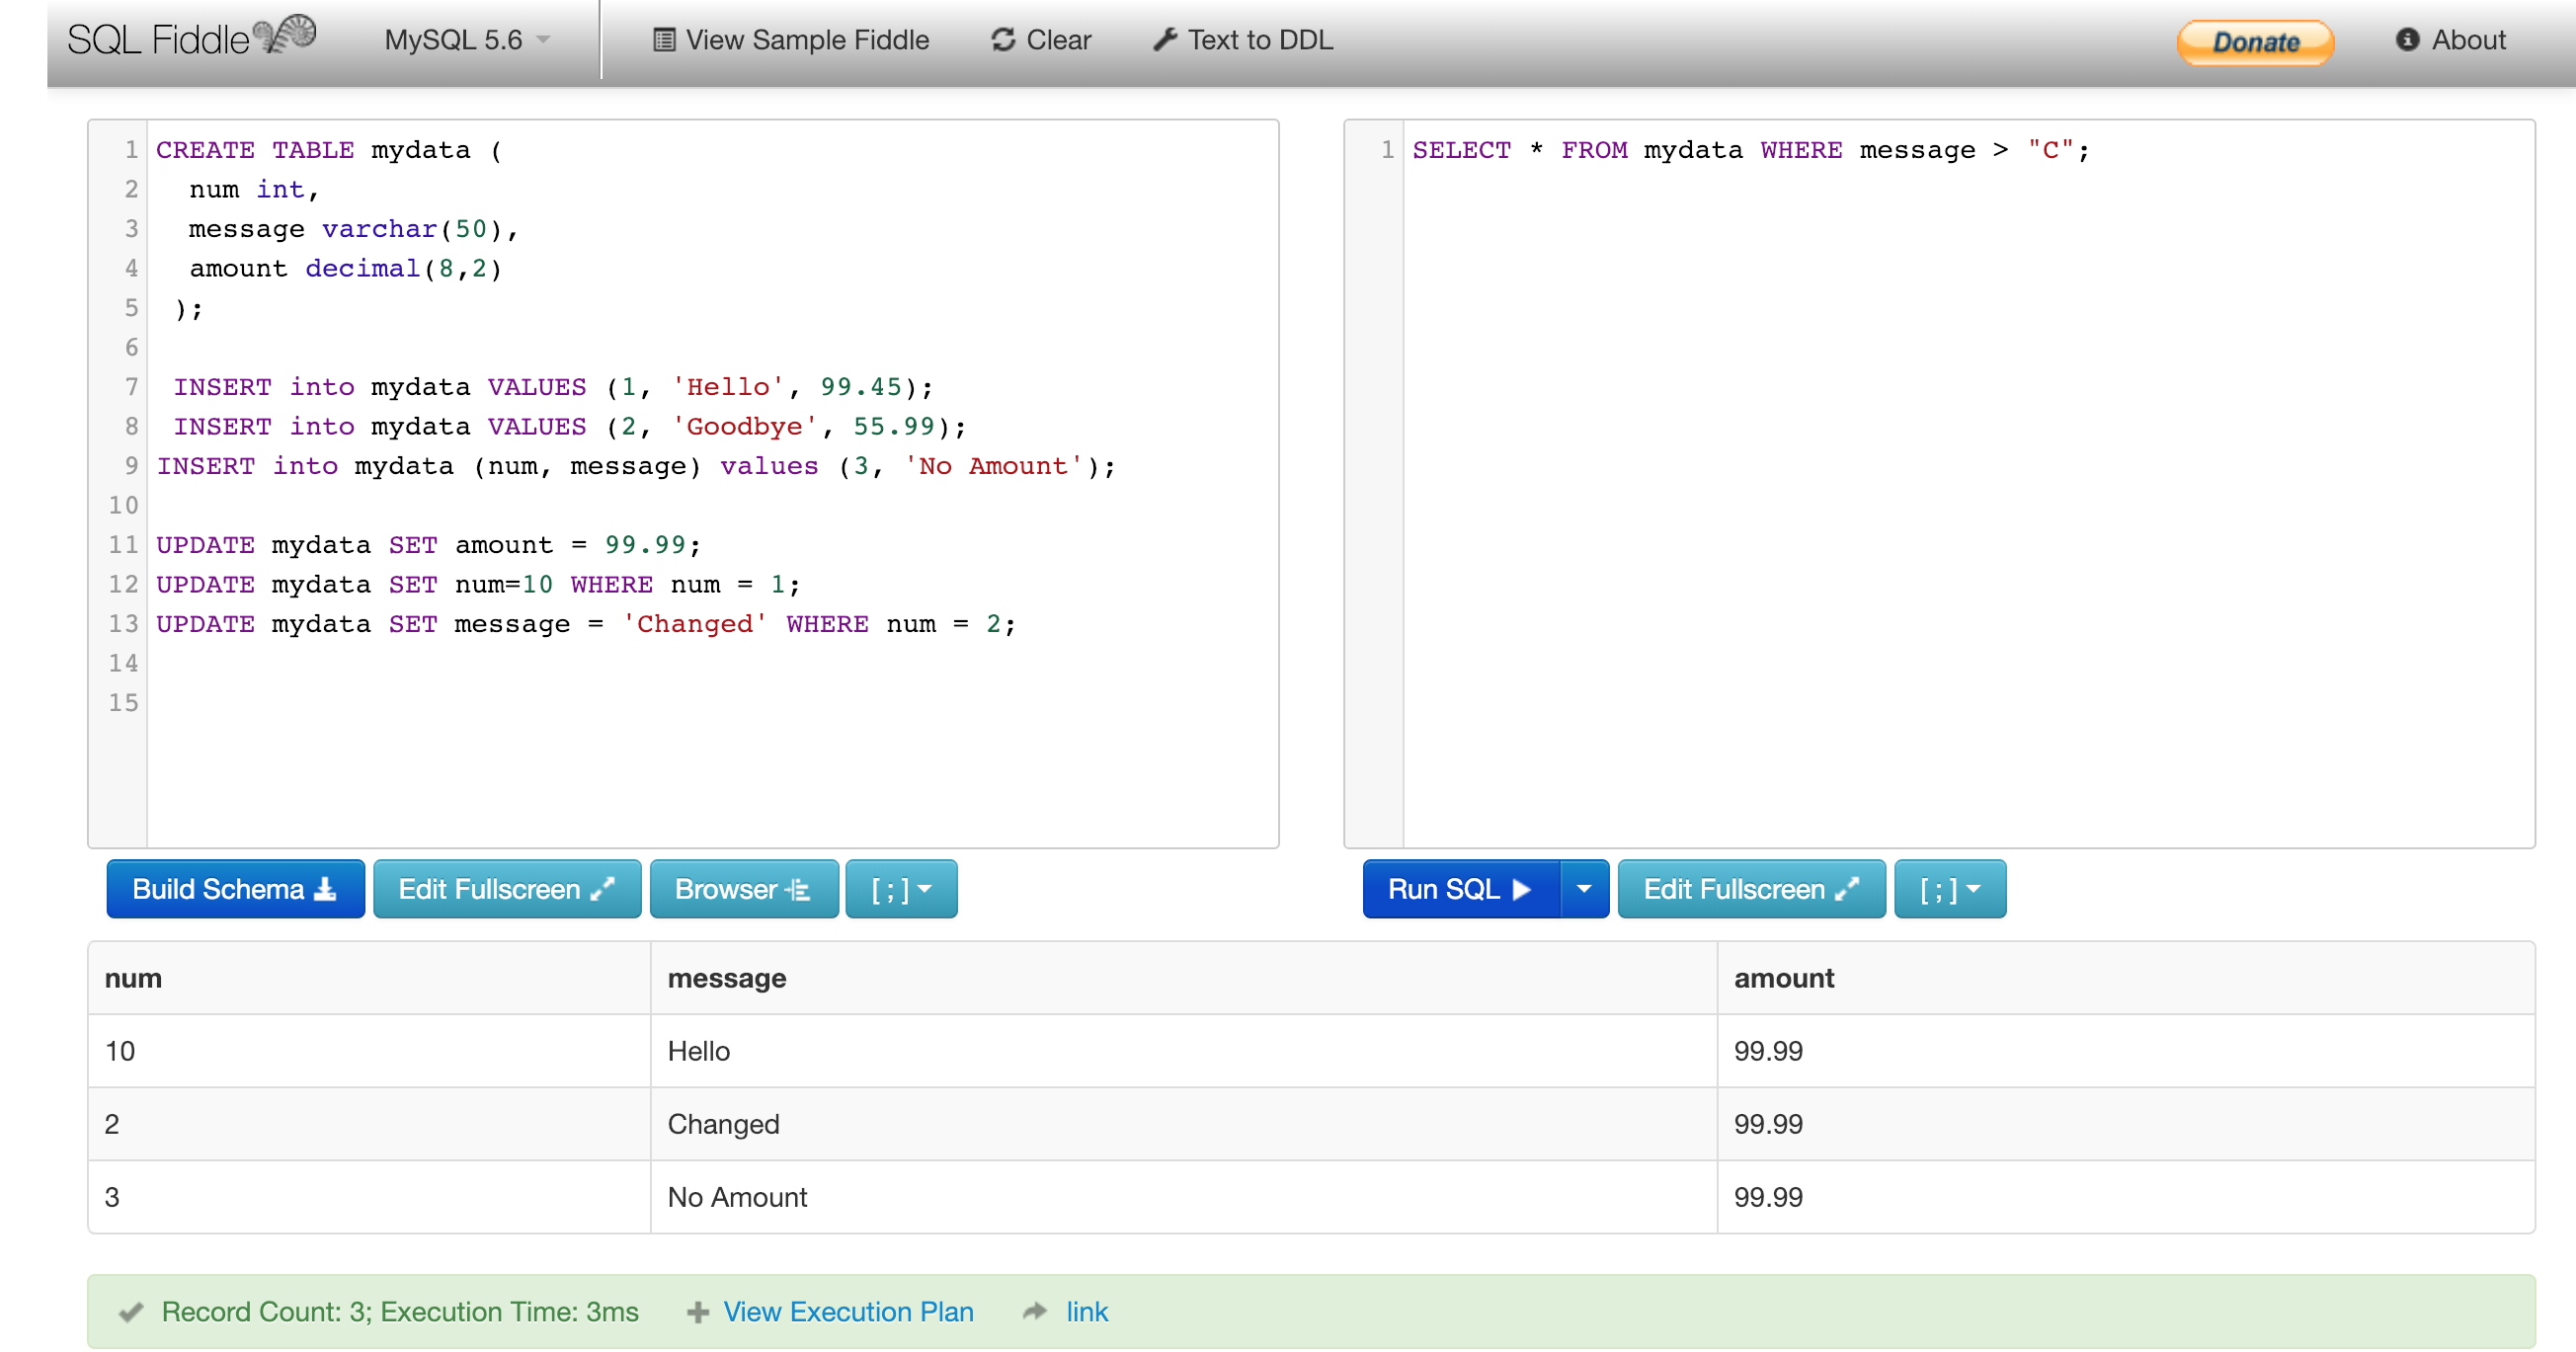
\includegraphics[width=0.99\textwidth]{img/mydataGc}
%\end{center}
%}

\frame{
Using $>$ on numbers:
  \begin{center}
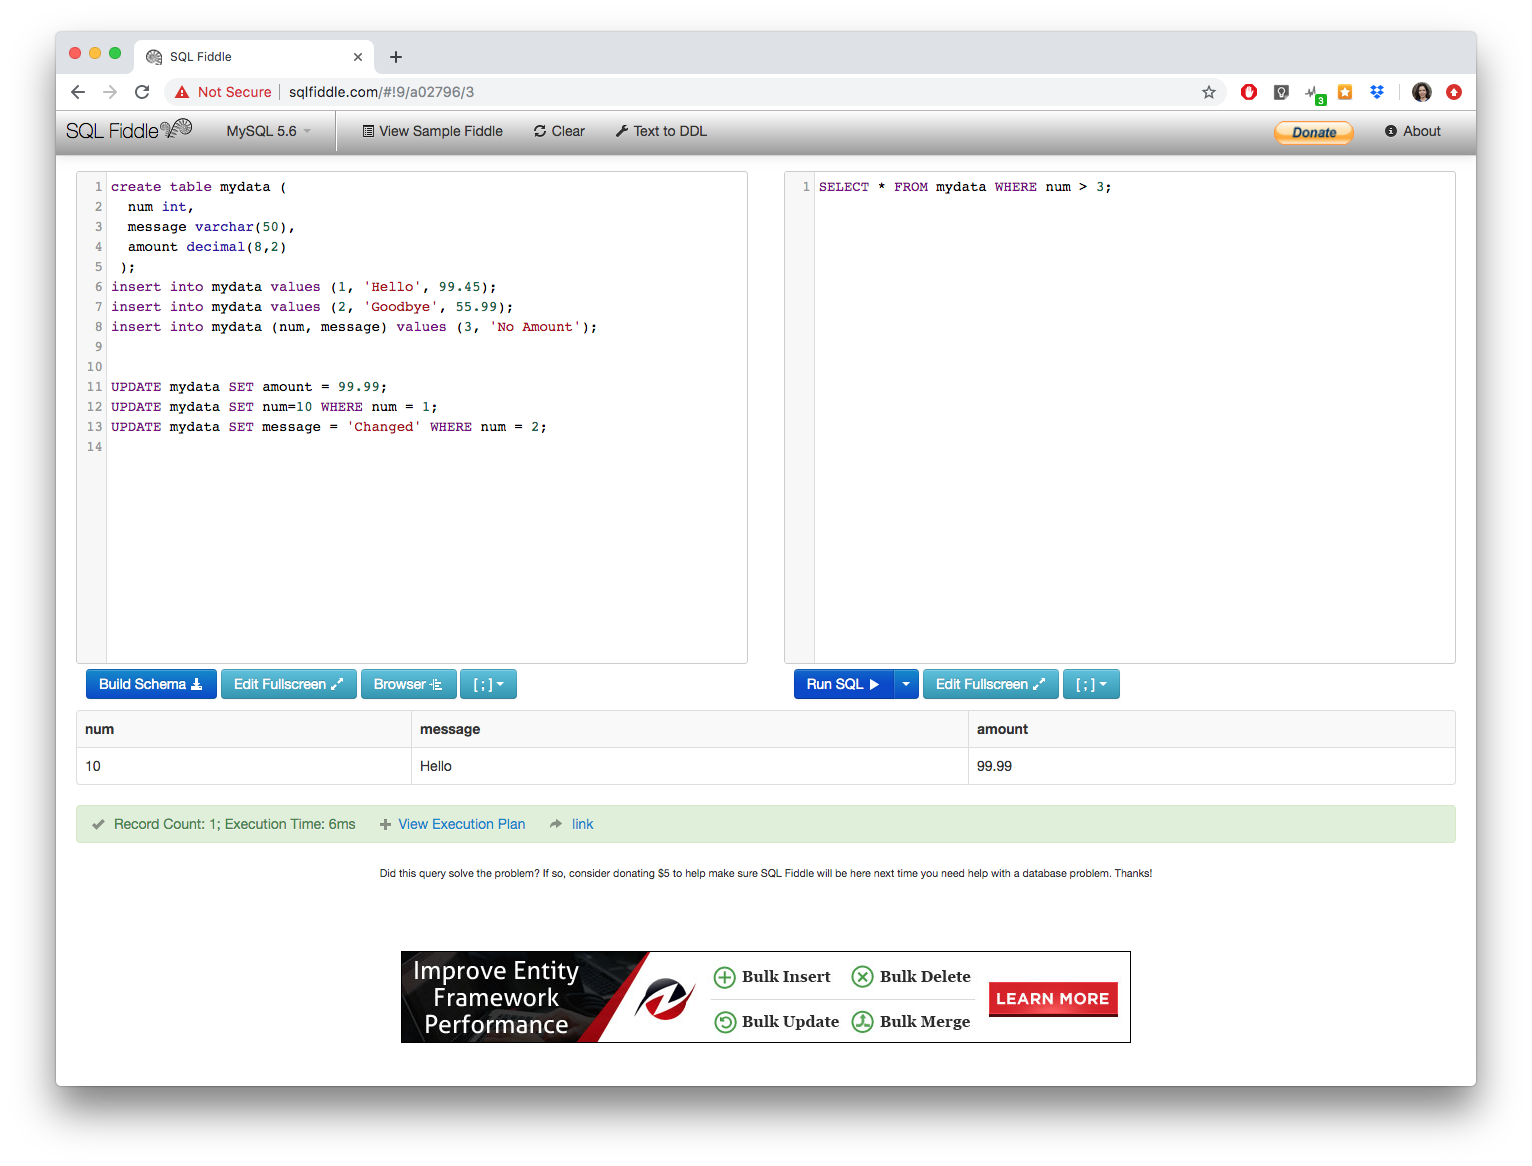
\includegraphics[width=0.99\textwidth]{img/greatnum}
\end{center}
}






\frame{
\ft{ Delete all rows}
Removing all rows and querying all the data from {\tt mydata} will return zero records.
  \begin{center}
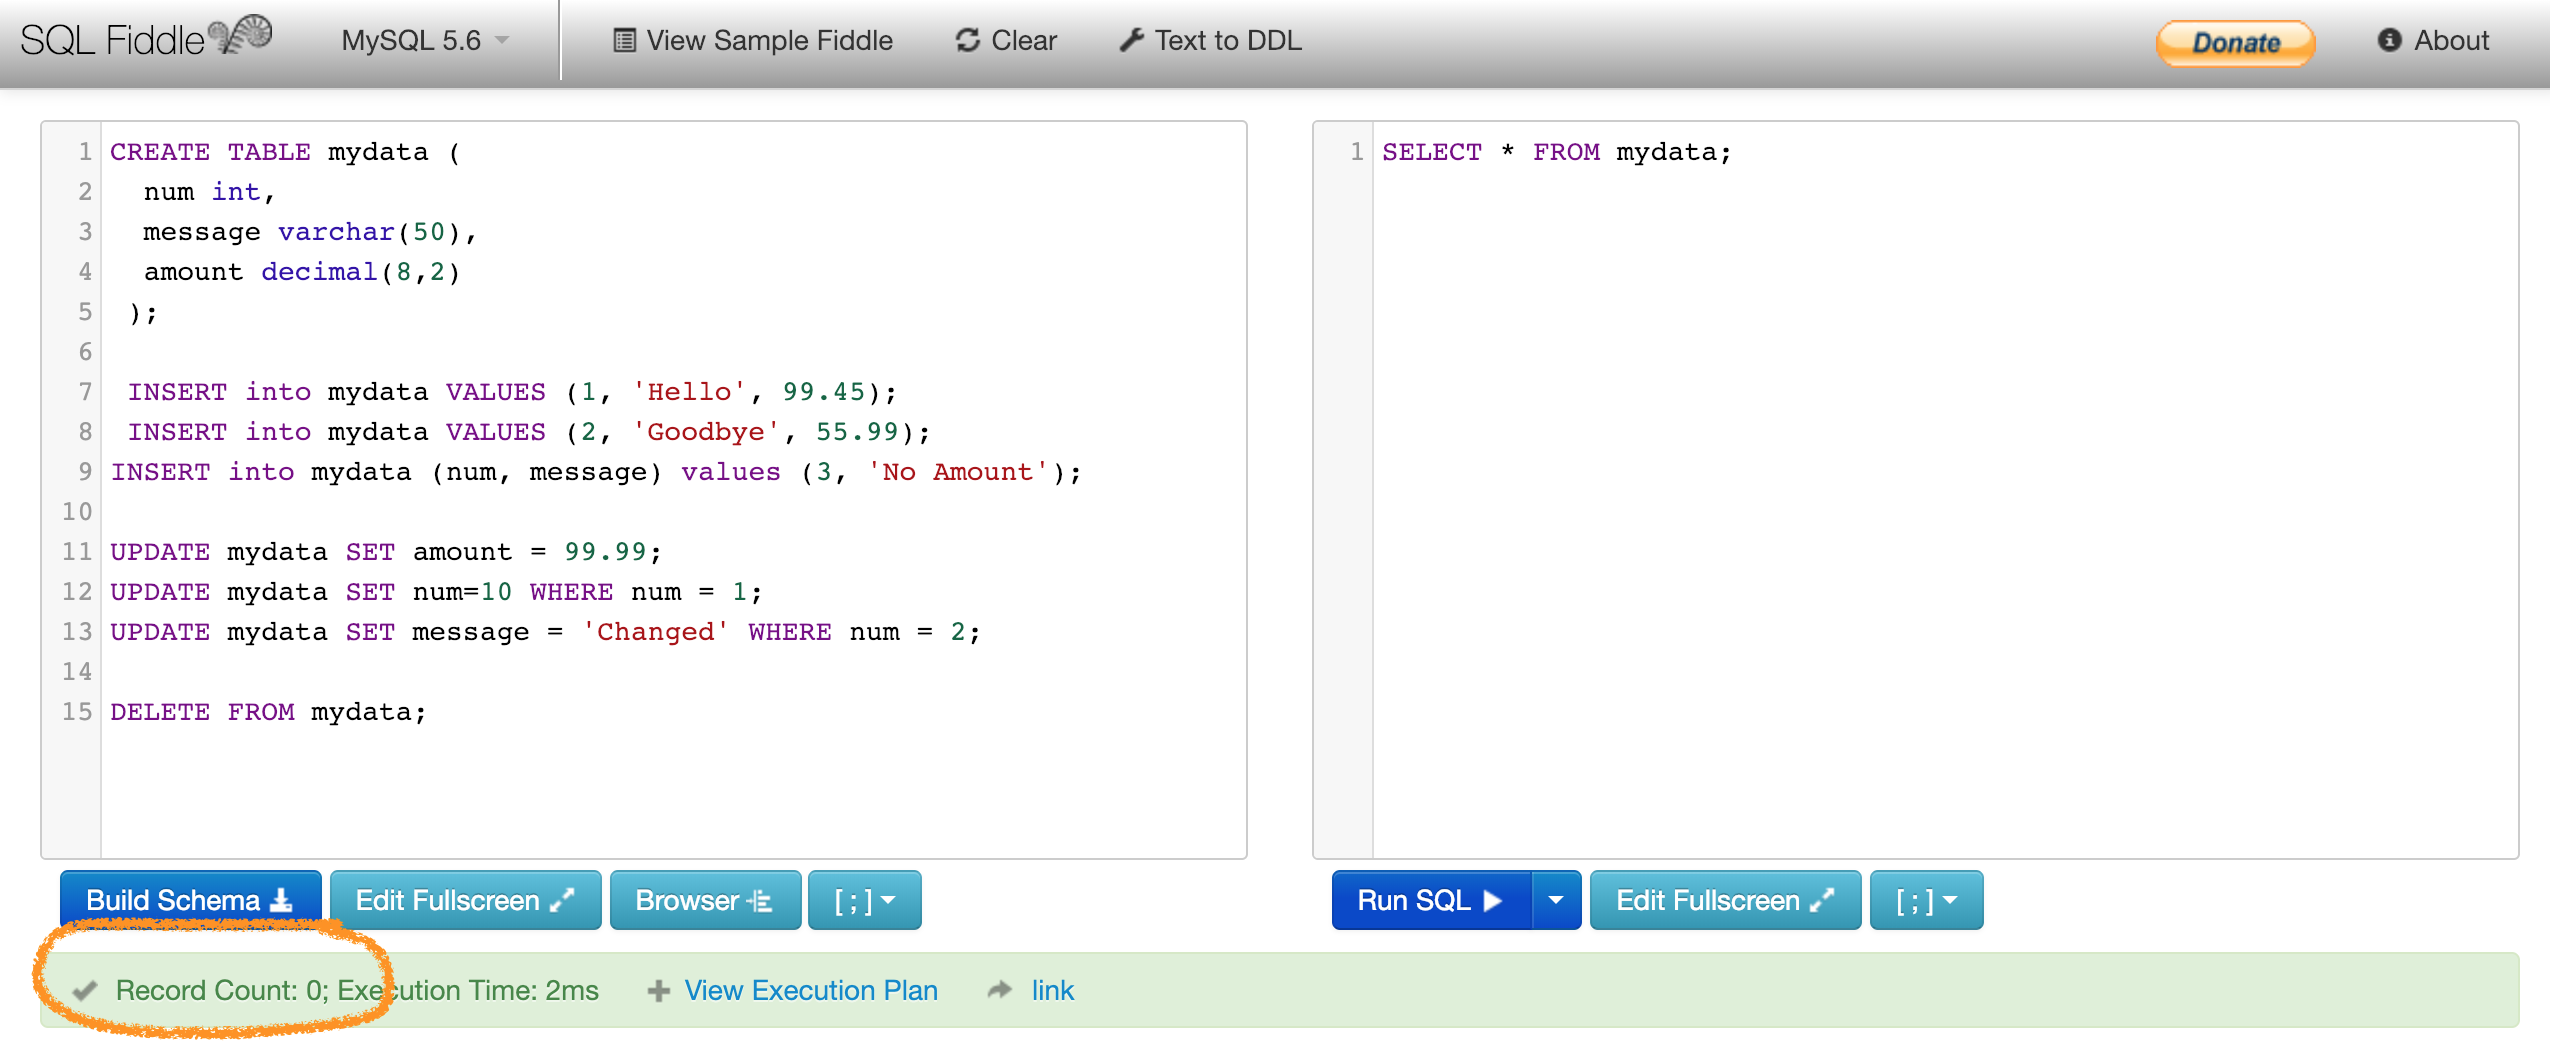
\includegraphics[width=0.99\textwidth]{img/noRec}
\end{center}
}





\begin{frame}[fragile]{{\tt DROP TABLE}}

When we delete all the records from a table, that table still exists (its just empty).
\vfill
The command \command{DROP TABLE} is used to delete the table and \emph{all its data} from the database. An example of usage:

$$ \command{DROP TABLE } { \tt emp;}$$

\begin{alertblock}
{Warning} The database does not confirm if you really want to drop the table and delete its data.  The effect of the command is immediate.
\end{alertblock}
\end{frame}

\begin{frame}{Create Tables Question}
\begin{example}
 How many of the following statements are TRUE?
\begin{enumerate}
\item Each field in the CREATE TABLE statement is separated by a comma.
\item The data type for a field is optional.
\item You can create two tables in a database with the same name.
\item A table will not be dropped (with DROP TABLE) if it contains data.
\end{enumerate}
\begin{multicols}{5}
\begin{enumerate}[A)]
\item 0 
\item 1
\item 2
\item 3
\item 4
\end{enumerate}
\end{multicols}
\end{example}
\end{frame}


\begin{frame}<handout:0>{Create Tables Question}
\begin{block}
{Answer} How many of the following statements are TRUE?
\begin{enumerate}
\item  {\color<1->{ForestGreen}{Each field in the CREATE TABLE statement is separated by a comma.}}
\item  {\color<2->{red}{The data type for a field is optional.}}
\item  {\color<3->{red}{You can create two tables in a database with the same name.}}
\item  {\color<4->{red}{A table will not be dropped (with DROP TABLE) if it contains data.}}
\end{enumerate}
\begin{multicols}{5}
\begin{enumerate}[A)]
\item 0 
\item \textbf<5>{\textit<5>{{\color<5>{iyellow}{1}}}}
\item 2
\item 3
\item 4
\end{enumerate}
\end{multicols}
\end{block}
\end{frame}



\begin{frame}
\begin{example}
[Insert Question] How many of the following statements are TRUE?
\begin{enumerate}
\item You must always specify the fields being inserted with INSERT statement. 
\item If you list the fields, the fields must be in the same order as the table.
\item If you do not provide a value for a number field, it will default to 1.
\item Number data items are enclosed in single quotes.
\end{enumerate}
\begin{multicols}{5}
\begin{enumerate}[A)]
\item 0 
\item 1
\item 2
\item 3
\item 4
\end{enumerate}
\end{multicols}
\end{example}
\end{frame}


\begin{frame}<handout:0>
\begin{block}
{Answer} How many of the following statements are TRUE?
\begin{enumerate}
\item {\color<1->{red}{You must always specify the fields being inserted with INSERT statement. }}
\item {\color<2->{red}{If you list the fields, the fields must be in the same order as the table.}}
\item {\color<3->{red}{If you do not provide a value for a number field, it will default to 1.}}
\item {\color<4->{red}{Number data items are enclosed in single quotes.}}
\end{enumerate}
\begin{multicols}{5}
\begin{enumerate}[A)]
\item \textbf<5>{\textit<5>{{\color<5>{iyellow}{0}}}} 
\item 1
\item 2
\item 3
\item 4
\end{enumerate}
\end{multicols}
\end{block}
\end{frame}

\frame{
\begin{example}
[Update Question] How many of the following statements are TRUE?
\begin{enumerate}
\item You may update more than one row at a time.
\item If the UPDATE has no WHERE clause, it updates all rows.
\item You may update zero or more rows using a UPDATE statement.
\item UPDATE may change more than one data value (column) in a row.
\end{enumerate}
\begin{multicols}{5}
\begin{enumerate}[A)]
\item 0
\item 1
\item 2
\item 3
\item 4
\end{enumerate}
\end{multicols}
\end{example}
}

\frame<handout:0>{
\begin{block}
{Answer} How many of the following statements are TRUE?
\begin{enumerate}
\item {\color<1->{ForestGreen}{You may update more than one row at a time.}}
\item {\color<2->{ForestGreen}{If the UPDATE has no WHERE clause, it updates all rows.}}
\item {\color<3->{ForestGreen}{You may update zero or more rows using a UPDATE statement.}}
\item {\color<4->{ForestGreen}{UPDATE may change more than one data value (column) in a row.} \only<4>{(use commas to separate parameters)}}
\end{enumerate}
\begin{multicols}{5}
\begin{enumerate}[A)]
\item 0
\item 1
\item 2
\item 3
\item \textbf<4>{\textit<4>{{\color<4>{iyellow}{4}}}} 
\end{enumerate}
\end{multicols}
\end{block}
}

\frame{
\begin{example}
[Delete Question] How many of the following statements are TRUE?
\begin{enumerate}
\item A DELETE with no WHERE clause will delete all rows.
\item The DELETE keyword is case-sensitive.
\item It is possible to DELETE zero or more rows using a WHERE clause.
%\item A DELETE statement may delete zero rows when executed.
\item {\tt DELETE mydata} will delete the entire table and its data.
\end{enumerate}
\begin{multicols}{5}
\begin{enumerate}[A)]
\item 0
\item 1
\item 2
\item 3
\item 4
\end{enumerate}
\end{multicols}
\end{example}
}


\frame<handout:0>{
\begin{block}
{Answer} How many of the following statements are TRUE?
\begin{enumerate}
\item {\color<1->{ForestGreen}{A DELETE with no WHERE clause will delete all rows.}}
\item {\color<2->{red}{The DELETE keyword is case-sensitive.}}
\item {\color<3->{ForestGreen}{It is possible to DELETE zero or more rows using a WHERE clause.}}
\item {\color<4->{red}{ {\tt DELETE mydata} will delete the entire table and its data.} \only<4> {for this we need DROP table}}
\end{enumerate}
\begin{multicols}{5}
\begin{enumerate}[A)]
\item 0
\item 1
\item \textbf<4>{\textit<4>{{\color<4>{iyellow}{2}}}} 
\item 3
\item 4
\end{enumerate}
\end{multicols}
\end{block}
}


%\begin{frame}
%  {Questions}
%
%  \nocite{lorem,ipsum}
%  \bibliographystyle{plain}
%  \bibliography{../demo}
%
%\end{frame}

\end{document}

